% Paper based on the master's thesis (../thesis/).
% Class: SIAM siamart251216 (Dec 2025). Do not edit siamart251216.cls or siamplain.bst.
% Build: latexmk main.tex   (pdflatex + bibtex)
\documentclass[review,onefignum,onetabnum]{siamart251216}

% ---------------------------------------------------------------- packages
\usepackage{amsfonts}
\usepackage{graphicx}
\usepackage{subcaption}
\usepackage{booktabs}
\usepackage{multirow}
\usepackage[dvipsnames]{xcolor}
\usepackage{tikz}
\usetikzlibrary{calc}
\usepackage{algorithm}
\usepackage{algpseudocode}
\renewcommand{\algorithmicrequire}{\textbf{Input:}}
\renewcommand{\algorithmicensure}{\textbf{Output:}}

\graphicspath{{images/}}

% Serial/Oxford comma in \cref lists
\newcommand{\creflastconjunction}{, and~}

% ---------------------------------------------------------------- theorems
\newsiamremark{remark}{Remark}
\renewtheorem{lemma}[theorem]{Lemma}
\renewtheorem{corollary}[theorem]{Corollary}
\renewtheorem{proposition}[theorem]{Proposition}
\renewtheorem{definition}[theorem]{Definition}

% ---------------------------------------------------------------- macros
\DeclareMathOperator{\diag}{diag}

% ---------------------------------------------------------------- title
\headers{Low-rank methods for PDE-based inverse problems}{E. J. Severinsen, O. L. Elvetun, and J. Kusch}

\title{Efficient Low-Rank Methods for PDE-Based Inverse Problems\thanks{Submitted to the editors DATE.}}

% TODO: confirm author list, order, and affiliations with supervisors.
\author{Elias Jegervatn Severinsen\thanks{Faculty of Science and Technology,
  Norwegian University of Life Sciences, {\AA}s, Norway
  (\email{elias.j.severinsen@gmail.com}).}
\and Ole Løseth Elvetun\footnotemark[2]
\and Jonas Kusch\footnotemark[2]}

\ifpdf
\hypersetup{
  pdftitle={Efficient Low-Rank Methods for PDE-Based Inverse Problems},
  pdfauthor={E. J. Severinsen, O. L. Elvetun, and J. Kusch}
}
\fi

\begin{document}

\maketitle

\begin{abstract}
% Problem context
We study source identification as an elliptic PDE-constrained inverse problem, where the forward operator has rapid decay of singular values and a large nullspace, making solutions unstable and non-unique. The use of Tikhonov regularization results in biased solutions, concentrating reconstructions near the boundary of the domain regardless of the true source location. True sources are often sparse, yet Tikhonov yields smooth reconstructions, blending distinct sources into connected regions.

% Gap
Elvetun and Nielsen correct the bias by applying a regularization operator, but the procedure requires explicit assembly of the forward operator and its singular value decomposition (SVD), making it infeasible at scale. It also suffers from the same smoothing issues as the Tikhonov method, making low-rank solutions a more natural approach for sparse sources. Dynamical low-rank approximation (DLRA) provides a robust framework for computing them but converges slowly for ill-posed problems.

% Contribution
We propose a matrix-free variant of the randomized SVD (rSVD), avoiding explicit construction of the forward operator, and making the weighted Tikhonov approach scalable. We also apply conjugate gradient (CG) within the DLRA framework (DLRA-CG) to accelerate convergence and recover sparse sources.

% Key results
We apply the matrix-free rSVD approach to previously inaccessible problems with no significant loss in reconstruction quality. Using DLRA-CG, we recover low-rank solutions that separate distinct sources more clearly and achieve lower reconstruction error than full-rank weighted Tikhonov. The method converges substantially faster than DLRA.

% Takeaways
Together, these contributions make large-scale sparse source identification possible, addressing the computational cost of the weighted Tikhonov approach and the tendency of these methods to blur distinct sources.
\end{abstract}

\begin{keywords}
  inverse source problems, Tikhonov regularization, randomized SVD,
  dynamical low-rank approximation, conjugate gradient
\end{keywords}

\begin{MSCcodes}
  % TODO: e.g. 65F55, 65N21, 65K10, 35R30
\end{MSCcodes}

% Tentative outline; mapping to thesis chapters in comments.
\section{Introduction}
\label{sec:intro}

% Source: thesis/sections/1_introduction.tex

% Motivation
Elliptic partial differential equations (PDEs) model steady-state problems such as electrical potential, heat conduction, and diffusion processes \cite{straussPartialDifferentialEquations2007}, and have applications in engineering, finance, and environmental science, among others \cite{evansPartialDifferentialEquations2010,pavliotisStochasticProcessesApplications2014}.

% Problem formulation
We study source identification constrained by an elliptic PDE: given a domain $\Omega$ with boundary $\partial\Omega$ and boundary observations $y = u|_{\partial\Omega}$ of the solution $u = \mathcal{S}f$, where $\mathcal{S}$ is the solution operator of the PDE, we seek to recover the unknown interior source $f$. This leads to an inverse problem of the form
\begin{equation}\label{eq:problem}
    \min_{f} \left\| u - y \right\|_{L^2(\partial\Omega)}^2
    + \lambda^2 \left\| W f \right\|_{L^2(\Omega)}^2
\end{equation}
subject to
\begin{equation}\label{eq:pde}
    \begin{aligned}
    -\nabla \cdot \sigma\nabla u + c u &= f \quad \text{in } \Omega, \\
    \frac{\partial u}{\partial n} &= 0 \quad \text{on } \partial\Omega.
    \end{aligned}
\end{equation}
Here, $\lambda$ is a regularization parameter, $W$ is the regularization weight operator, $\sigma$ is the diffusion coefficient and $c$ is the reaction coefficient. We refer to the operator $\mathcal{K}: f \mapsto u|_{\partial\Omega}$ as the forward operator, mapping the source to the boundary values of the solution. The Neumann boundary condition in Equation~\eqref{eq:pde} ensures no flow over the boundary.

This problem arises in applications such as inverse imaging, crack determination, and electromagnetic brain mapping \cite{nielsenComputingIschemicRegions2013,elulGenesisEEG1971,PDFRecoveryCracks}. For example, in electroencephalography (EEG), it can be used for improved understanding and treatment of brain disorders like Alzheimer's, Parkinson's, and depression \cite{elulGenesisEEG1971, ElectromagneticBrainMapping}.

However, source identification problems of this form are ill-posed, as the operator $\mathcal K$ has a rapid decay of singular values and a large nullspace. Reconstructions are therefore unstable and non-unique \cite{hansen2010discrete}. Standard approaches like Tikhonov regularization introduce bias to the reconstructions, making solutions appear near the domain boundary regardless of the true location of the source \cite{elvetunRegularizationOperatorSource2020}. True sources are often sparse, yet Tikhonov smooths reconstructions, blurring distinct sources into connected regions.

% Prior work
Elvetun and Nielsen address the localization bias of Tikhonov by introducing regularization weights $W$ that use information about the forward operator $\mathcal{K}$ to correct the bias \cite{elvetunRegularizationOperatorSource2020}. This method shows promising results, correctly identifying the position of one or multiple sources from boundary data \cite{elvetunRegularizationOperatorSource2020,elvetunModifiedTikhonovRegularization2020}. However, their approach requires explicit knowledge about $\mathcal{K}$ and its SVD, making it computationally infeasible for large-scale problems. Also, for sparse sources, Elvetun and Nielsen's method still suffers from the same smoothing problems as Tikhonov, blurring the reconstructions and blending distinct sources \cite{elvetunModifiedTikhonovRegularization2020}. 
Since sparse sources are naturally represented by low-rank matrices, recovering low-rank solutions is an appropriate objective. Dynamical low-rank approximation (DLRA) provides a robust framework for this \cite{schotthoferLowrankLotteryTickets2022}, but existing methods rely on first-order updates such as Adam \cite{kingmaAdamMethodStochastic2017} and steepest descent, which converge slowly for ill-conditioned problems \cite{chong2023introduction,hansen2010discrete,nocedal2006numerical}.

% Contribution
We propose two methods. The first is a matrix-free variant of the randomized SVD (rSVD) that computes a rank-$k$ factorization of the forward operator, avoiding its explicit formation and addressing the computational cost of Elvetun and Nielsen's 
weights. The second recovers sparse, rank-$r$ sources where Tikhonov smooths, converging substantially faster than existing DLRA methods. The ranks $k$ and $r$ are independent: $k$ is the approximation rank of $\mathcal{K}$, and $r$ is the rank of the matrix representation of the source $f$.

The first method uses random sampling of $\operatorname{range}(K)$ to compute an approximate rank-$k$ SVD $K \approx U \Sigma V^T$ of the discretized forward operator, which can then be used to solve the weighted Tikhonov problem at large scale. It relies on applications of the forward operator $K$ and adjoint $K^*$, which can be done efficiently by pre-computing sparse Cholesky factorizations of the PDE operator. The method is applied to previously computationally infeasible problems without a significant loss in reconstruction quality.

The second method uses conjugate gradient (CG) within the DLRA framework to accelerate convergence and recover sparse sources. It adapts the DLRA method proposed by Schotthöfer et al. for neural network training \cite{schotthoferLowrankLotteryTickets2022} to the setting of sparse source identification. The convex optimization problem of Equation~\eqref{eq:problem}, with Elvetun and Nielsen's $W$, defines an objective function $\Phi$ with a symmetric positive definite (SPD) Hessian $H$, for which CG is particularly well-suited \cite{hestenesMethodsConjugateGradients1952,fletcherFunctionMinimizationConjugate1964}. The resulting method converges substantially faster than DLRA with steepest descent and yields rank-$r$ solutions that separate distinct sources more clearly than full-rank weighted Tikhonov.

The proposed methods are not limited to the particular problem studied in this thesis. The matrix-free rSVD method is well suited for a broader class of elliptic source identification problems, where the forward operators have rapid spectral decay \cite{evansPartialDifferentialEquations2010,engl1996regularization}. The DLRA-CG method can be used for low-rank problems with a quadratic objective function and an SPD Hessian.

% Paper outline
The remainder of this paper is organized as follows. Section~\ref{sec:setup} introduces the inverse problem, its finite-element discretization, and the Elvetun--Nielsen regularization weights. Section~\ref{sec:rsvd} presents the matrix-free rSVD of the forward operator and its adjoint variant. Section~\ref{sec:dlracg} introduces DLRA-CG, including restarts and preconditioning. Section~\ref{sec:experiments} compares computational cost, reconstruction quality, and convergence using the numerical experiments. Sections~\ref{sec:conclusions} and~\ref{sec:conclusion} discuss the results and summarize the findings, limitations, and future directions.
       % thesis ch. 1
\section{Problem setup}
\label{sec:setup}

% Source: thesis/sections/2_mathematical_background.tex
% \section{Mathematical background}\label{sec:mathematical_background}

\subsection{The forward operator}
\begin{figure}[htbp]
    \centering
    \begin{tikzpicture}[
        >=stealth,
        line width=0.9pt,
        every node/.style={font=\large}
    ]
    % Boxes
    \draw (0,0) rectangle (2,2);
    \draw (3,0) rectangle (5,2);
    \draw (6,0) rectangle (8,2);
    
    % Space labels H^1
    \node at (1,-0.5) {$L^2(\Omega)$};
    \node at (4,-0.5) {$H^1(\Omega)$};
    \node at (7,-0.5) {$L^2(\partial\Omega)$};
    
    % f, u, and u|_dOmega points
    \node (f) at (1,1) {$f$};
    \node (u) at (4,1) {$u$};
    \node (g) at (7,1) {$u|_{\partial\Omega}$};
    
    % Operator S
    \draw[->]
      (f) -- (u)
      node[midway, below, xshift=0.0mm] {$\mathcal S$};
    
    % Operator T
    \draw[->]
      (u) -- (g)
      node[midway, below, xshift=1.0mm] {$\mathcal T$};
    
    % Operator K
    \draw[->]
      (f) to[out=45, in=140]
      node[midway, above] {$\mathcal{K}$}
      (g);
    \end{tikzpicture}
    \caption{The forward operator $\mathcal K = \mathcal T \circ \mathcal S$ maps $f$ to $u|_{\partial\Omega}$.}
    \label{fig:forward_operator}
\end{figure}
Let $\Omega \subset \mathbb R^2$ be a bounded domain with boundary $\partial \Omega$, and consider the boundary value problem (BVP) in Equation~\eqref{eq:pde}. The coefficient $\sigma = \sigma(x) > 0$ denotes the diffusion coefficient and determines the rate and direction of diffusion in the problem. It may be either scalar-valued or matrix-valued. In the latter case, we assume that $\sigma(x)$ is symmetric and positive definite to keep the problem elliptic. The reaction coefficient $c = c(x) > 0$ describes the absorption or decay within the problem. Finally, $f = f(x)$ denotes the source term, which is the unknown input of the inverse problem.

Equation~\eqref{eq:pde} is a linear diffusion-reaction problem with Neumann boundary conditions, and defines a mapping
\begin{equation}\label{eq:S_cont}
    \mathcal S: L^2(\Omega) \rightarrow H^1(\Omega), \quad \mathcal{S} f = u.
\end{equation}
Here, $L^2(\Omega)$ is the space of square integrable functions, and $H^1(\Omega)$ is the Sobolev space of functions in $L^2(\Omega)$ whose weak first derivatives also belong to $L^2(\Omega)$ \cite{quarteroniNumericalModelsDifferential2014}.

To model boundary observations, we introduce the trace operator
\begin{equation}\label{eq:trace}
    \mathcal T: H^1(\Omega) \rightarrow L^2(\partial\Omega), \quad \mathcal{T} u = u|_{\partial\Omega}.
\end{equation}
The term $\mathcal{T} u$ represents the boundary observations of the solution $u$.

The forward operator is then defined as the composition
\begin{equation}\label{eq:K}
    \mathcal K = \mathcal T \circ \mathcal S, \quad \mathcal{K} f = u|_{\partial\Omega},
\end{equation}
which is a mapping from the source function $f$ to the observed output $u|_{\partial\Omega} = \mathcal K f$ on the boundary $\partial \Omega$, see Figure~\ref{fig:forward_operator}.

The associated inverse problem can now be formulated as follows: given boundary data $u|_{\partial\Omega}$, determine a source function $f$ such that
\begin{equation*}
    \mathcal{K} f = u|_{\partial\Omega}.
\end{equation*}
Solving this problem computationally requires discretizing $\mathcal{K}$, understanding the ill-posedness of the resulting system, and regularizing it to obtain stable solutions, which we address in the following sections.


\subsubsection{Ill-posedness}\label{sec:ill_posedness}
A problem is said to be well-posed if its solution exists, is unique, and is stable in the sense that it depends continuously on the data, as formulated by Hadamard \cite{hansen2010discrete}. Denoting $y = u|_{\partial\Omega}$, the inverse problem $\mathcal{K}f = y$ is ill-posed.

The null space of $\mathcal{K}$ is non-trivial: any $f_0$ satisfying $\mathcal{K}f_0 = 0$ can be added to a solution without changing the boundary data $y$. The solution is therefore not unique.

The instability of the solution $f$ is more severe in practice. The compactness of $\mathcal{K}$, and the ellipticity of the PDE in Equation~\eqref{eq:pde}, result in a rapid decay of its singular values towards zero \cite{evansPartialDifferentialEquations2010,engl1996regularization}. Solution components corresponding to small singular values are strongly suppressed by the forward operator and cannot be recovered from noisy data: a small perturbation in $y$ produces a large error in the reconstructed source. This motivates the regularized formulation stated in Equation~\eqref{eq:problem}.


\subsection{Finite element discretization}
\subsubsection{The finite element method}
\begin{figure}[htbp]
    \centering
    \begin{tikzpicture}[
        >=stealth,
        line width=0.9pt,
        every node/.style={font=\large}
    ]
    % Left: continuous domain Omega
    \begin{scope}[shift={(0,0)}]
      % Draw a smooth-ish domain
      \draw[thick]
        plot [smooth cycle, tension=0.5]
        coordinates {
          (0,0)
          (2.2,0.3)
          (2.6,1.6)
          (1.6,2.6)
          (0.4,2.2)
          (-0.4,1.2)
        };
      % Label
      \node at (1,-0.5) {\Large $\Omega$};
    \end{scope}
    
    % Middle arrow
    \begin{scope}[shift={(4.2,1.2)}]
        \draw[very thick,->] (-1.2,0) -- (1.2,0);
        \node[above] at (0,0) {Triangulation};
    \end{scope}
    
    % Right: triangulated mesh M
    \begin{scope}[shift={(6.2,0)}]
        % Outer polygon (approximation of Omega)
        \coordinate (A) at (0,0);
        \coordinate (B) at (2.4,0.3);
        \coordinate (C) at (2.8,1.6);
        \coordinate (D) at (1.7,2.7);
        \coordinate (E) at (0.3,2.3);
        \coordinate (F) at (-0.4,1.2);
        % Boundary
        \draw[thick] (A)--(B)--(C)--(D)--(E)--(F)--cycle;
        % Some interior points
        \coordinate (P1) at (1.1,0.7);
        \coordinate (P2) at (1.9,1.2);
        \coordinate (P3) at (1.2,1.8);
        \coordinate (P4) at (0.4,1.4);
        % Draw triangulation
        \draw (A)--(P1)--(B);
        \draw (B)--(P2)--(C);
        \draw (C)--(P3)--(D);
        \draw (D)--(P3)--(E);
        \draw (E)--(P4)--(F);
        \draw (F)--(P4)--(A);
        \draw (P1)--(P2)--(P3)--(P4)--cycle;
        \draw (P1)--(P3);
        \draw (P2)--(P4);
        % Label
        \node at (1.2,-0.5) {\Large $\mathcal M$};
    \end{scope}
    \end{tikzpicture}
    \caption{The triangulation $\mathcal{M}$ (the mesh) of $\Omega$. $\mathcal{M}$ is made up of $N$ nodes located at the vertices (corners) of the triangles.}
    \label{fig:triangulation}
\end{figure}
Consider the PDE in Equation~\eqref{eq:pde}. Multiplying the equation by a test function $v \in H^1(\Omega)$, integrating over $\Omega$, and applying Green's identity yields the weak formulation: find $u \in H^1(\Omega)$ such that
\begin{equation}\label{eq:variational_formulation}
    \int_{\Omega} (\sigma \nabla u \cdot \nabla v + c u v) \, dx = \int_{\Omega} f v \, dx,
    \text{ for all } v \in H^1(\Omega).
\end{equation}
For details on the derivation, see Section~4 in Larson and Bengzon \cite{larsonFiniteElementMethod2013}.

Let $\mathcal M$ be a triangulation of $\Omega$ made up of $N$ nodes, with $N_b$ boundary nodes, see Figure~\ref{fig:triangulation} as an example. Introduce the finite element space $V_h \subset H^1(\Omega)$,
\begin{equation}\label{eq:fem_space}
    V_h = \{v \in C^0(\Omega) : v|_M \text{ is linear for all } M \in \mathcal M \}.
\end{equation}
Let $\{\phi_1, \dots, \phi_N\}$ denote a basis for $V_h$, so that
\begin{equation*}
    V_h = \operatorname{span}\{ \phi_1, \dots, \phi_N \}.
\end{equation*}
The basis functions $\phi_i$ are piecewise linear hat functions associated with the nodes of the mesh (see \cite[p.~51]{larsonFiniteElementMethod2013}).

The finite element approximation of \eqref{eq:variational_formulation} then reads: 
find $u_h \in V_h$ such that
 \begin{equation}\label{eq:fem_formulation}
    \int_{\Omega} (\sigma \nabla u_h \cdot \nabla v + c u_h v) \, dx = \int_{\Omega} f v \, dx,
    \text{ for all } v \in V_h.
\end{equation}


\subsubsection{The discrete forward operator}
To obtain a discrete representation of the forward operator 
$\mathcal{K} = \mathcal{T} \circ \mathcal{S}$, 
we discretize both the PDE operator $\mathcal{S}$ and the trace operator $\mathcal{T}$ using the finite element space $V_h$.

Let $f_h, u_h \in V_h$ denote the finite element approximations of $f$ and $u$, respectively. Since $V_h = \operatorname{span}\{\phi_1,\dots,\phi_N\}$, they can be written as
\begin{equation}\label{eq:uh_and_fh}
    f_h = \sum_{j=1}^{N} x_j \phi_j, \quad
    u_h = \sum_{j=1}^{N} u_j \phi_j, 
\end{equation}
with coefficient vectors $x = (x_1,\dots,x_N)^T$, $u = (u_1,\dots,u_N)^T$.

Inserting \eqref{eq:uh_and_fh} into the finite element formulation \eqref{eq:fem_formulation} and testing with the basis functions 
$\{\phi_i\}_{i=1}^N$ yields the linear system
\begin{equation}\label{eq:matrix_system}
    A_h u = M x,
\end{equation}
where $A_h \in \mathbb{R}^{N \times N}$ is the stiffness matrix and $M \in \mathbb{R}^{N \times N}$ the mass matrix, both symmetric positive definite \cite{larsonFiniteElementMethod2013}.
Equation~\eqref{eq:matrix_system} implies that the discrete PDE operator $S$ takes the form
\begin{equation*}
    S = A_h^{-1} M \in \mathbb{R}^{N \times N}.
\end{equation*}
Note that $S$ is a mapping of coefficient vectors: mapping $x$ to $u$.

The trace operator is discretized by a matrix 
$T \in \mathbb{R}^{N_b \times N}$ that extracts the boundary coefficients. If $y$ denotes the vector of boundary coefficients, then
\begin{equation*}
    y = T u.
\end{equation*}

Combining the discrete PDE and trace operators yields the matrix representation of the forward operator,
\begin{equation}\label{eq:discrete_K}
    K = T S = T A_h^{-1} M \in \mathbb{R}^{N_b \times N}.
\end{equation}


\subsubsection{Discrete inner product and norm}
Let $V_h$ be the finite element space introduced in Equation~\eqref{eq:fem_space} and let $f_h, g_h \in V_h$, with coefficient vectors $x, y \in \mathbb{R}^N$, respectively. The $L^2(\Omega)$ inner product of $f_h$ and $g_h$ can be written as
\begin{equation*}
    \langle f_h, g_h \rangle_{L^2(\Omega)} = x^T M y,
\end{equation*}
where $M$ is the mass matrix. 

This induces a discrete inner product on $\mathbb{R}^N$, with associated norm, defined by
\begin{equation}\label{eq:fem_norm}
    \langle x, y \rangle_M = x^T M y,
    \quad
    \| x \|_M = \sqrt{x^T M x}.
\end{equation}

Similarly, let $u, v \in \mathbb{R}^{N_b}$ 
denote coefficient vectors corresponding to the traces 
$u_h|_{\partial\Omega}$ and $v_h|_{\partial\Omega}$. The $L^2(\partial\Omega)$ inner product induces a discrete inner product and norm on $\mathbb{R}^{N_b}$, given by
\begin{equation}\label{eq:fem_norm_ds}
    \langle u, v \rangle_{M_{\partial}}
    = u^T M_{\partial} v,
    \quad
    \| u \|_{M_{\partial}}
    =
    \sqrt{u^T M_{\partial} u},
\end{equation}
where $M_\partial$ denotes the boundary mass matrix.


\subsubsection{The adjoint operator}
Let $\mathcal{K}: L^2(\Omega) \to L^2(\partial\Omega)$ be the bounded linear operator defined in Equation~\eqref{eq:K}. The adjoint operator $\mathcal{K}^*: L^2(\partial\Omega) \to L^2(\Omega)$ is the bounded linear operator satisfying
\begin{equation}\label{eq:K_star_cont}
    \langle \mathcal K f,\, g \rangle_{L^2(\partial\Omega)} =
    \langle f,\, \mathcal K^* g \rangle_{L^2(\Omega)},
\end{equation}
for all $f \in L^2(\Omega)$ and all $g \in L^2(\partial\Omega)$. Such an operator always exists for a bounded linear operator $\mathcal K$ mapping between two Hilbert spaces, see Section~3.9 in Kreyszig for a proof \cite{kreyszigIntroductoryFunctionalAnalysis1989}.

Using the definition in Equation~\eqref{eq:K_star_cont}, we get the weak formulation of $\mathcal{K}^*$ (the adjoint problem): find $w \in H^1(\Omega)$ such that
\begin{equation}\label{eq:variational_formulation_adjoint}
    \int_\Omega (\sigma \nabla w \cdot \nabla v + c w v) \, dx =
    \int_{\partial\Omega} g v \, ds,
    \text{ for all } v \in H^1(\Omega).
\end{equation}
To verify that $\mathcal K^* g = w$, let $u = \mathcal S f$. Testing Equation~\eqref{eq:variational_formulation} with $v = w$ and Equation~\eqref{eq:variational_formulation_adjoint} with $v = u$, and using the symmetry of $\sigma$, gives
\begin{equation*}
    \langle \mathcal K f, g \rangle_{L^2(\partial\Omega)}
    = \int_{\partial\Omega} g u \, ds
    = \int_\Omega f w \, dx
    = \langle f, w \rangle_{L^2(\Omega)}.
\end{equation*}
Thus $w$ satisfies the identity~\eqref{eq:K_star_cont}.

In the discrete case, under the inner products and norms defined in Equations~\eqref{eq:fem_norm} and~\eqref{eq:fem_norm_ds}, the adjoint operator $K^* \in \mathbb{R}^{N \times N_b}$ of $K \in \mathbb{R}^{N_b \times N}$ satisfies
\begin{equation}\label{eq:K_star_def}
    (K x)^T M_\partial y = x^T M K^* y,
\end{equation}
for all $x \in \mathbb R^N$ and all $y \in \mathbb R^{N_b}$.

Inserting the explicit representation of $K$ given in Equation~\eqref{eq:discrete_K} and using the symmetry of $A_h$ yields the matrix representation of $K^*$,
\begin{equation}\label{eq:discrete_K_star}
    K^* = A_h^{-1} T^T M_\partial,
\end{equation}
where $A_h$ is the stiffness matrix, $T$ the discrete trace operator, and $M_\partial$ the boundary mass matrix.


\subsection{Tikhonov regularization}
Let $A \in \mathbb{R}^{m \times n}$ and consider the inverse problem $Ax = y$. If $A$ is ill-conditioned, the matrix $A^T A$ in the normal equations $A^T A x = A^T y$ is also ill-conditioned, and small perturbations in $y$ 
cause large changes in the solution. Tikhonov regularization stabilizes the problem by solving
\begin{equation}\label{eq:tikhonov}
    \min_{x \in \mathbb{R}^n}
    \|Ax - y\|^2 + \lambda^2 \|Wx\|^2,
\end{equation}
where $\lambda \ge 0$ is the regularization parameter and $W \in \mathbb{R}^{n \times n}$ is the weight matrix. The normal equations of Equation~\eqref{eq:tikhonov} are $(A^T A + \lambda^2 W^T W) x = A^T y$, so if $W$ is diagonal with $\operatorname{diag}(W) > 0$ and $\lambda > 0$, then $(A^T A + \lambda^2 W^T W)$ is SPD, stabilizing the problem and making the solution unique.

The weights $W$ can include prior knowledge about the solution to penalize specific types of unwanted solutions \cite{hansen2010discrete}. With $W = I$, this is standard Tikhonov regularization.


\subsection{SVD and low-rank approximations}
The rapid decay of the singular values of $K$ makes it possible to approximate $K$ well by a low-rank matrix. Its right singular vectors also determine the regularization weights in Section~\ref{sec:the_discrete_inverse_problem}.

\subsubsection{Singular value decomposition}\label{sec:svd}
The singular value decomposition of a matrix $A\in\mathbb R^{m\times n}$ of rank $q$ is $A=U\Sigma V^T$, where $U\in\mathbb R^{m\times q}$ and $V\in\mathbb R^{n\times q}$ have orthonormal columns and $\Sigma=\operatorname{diag}(\sigma_1,\dots,\sigma_q)$ with $\sigma_1\ge\cdots\ge\sigma_q>0$. The columns $u_i$ and $v_i$ of $U$ and $V$ are the left and right singular vectors of $A$, respectively.

Keeping the first $k$ singular values and the corresponding singular vectors gives the truncated SVD (tSVD),
\begin{equation}\label{eq:tsvd}
    A_k = U_k\Sigma_k V_k^T.
\end{equation}
By the Eckart--Young--Mirsky theorem \cite{eckartApproximationOneMatrix1936}, $A_k$ is the best approximation of $A$, with its error in the spectral norm satisfying
\begin{equation}\label{eq:svd_error}
    \|A-A_k\|_2 = \min_{\operatorname{rank}(X)\le k}\|A-X\|_2 = \sigma_{k+1}.
\end{equation}
Truncating small singular values regularizes the pseudoinverse \cite{hansen2010discrete}. The tSVD also provides a reference for the randomized approximation of $K$ in Section~\ref{sec:rsvd}.


The Moore--Penrose pseudoinverse of $A$ is
\begin{equation}\label{eq:pseudoinverse}
    A^+ = V\Sigma^{-1}U^T,
\end{equation}
where $\Sigma^{-1}=\operatorname{diag}(1/\sigma_1,\dots,1/\sigma_q)$. For the least-squares problem $\min_x\|Ax-y\|_2$, $A^+y$ is the solution with the smallest Euclidean norm \cite[Section~5.5]{golubMatrixComputations4th2013}. The identity $A^+A=VV^T$ gives the orthogonal projection onto the row space of $A$, used below to compute the regularization weights.

For a nonsingular square matrix $A\in\mathbb R^{n\times n}$, the condition number in the spectral norm is $\kappa(A)=\sigma_1/\sigma_n$ \cite{hansen2010discrete}.


\subsubsection{Randomized SVD}
The randomized SVD is a technique used to compute a rank-$k$ approximation of an $m\times n$ matrix without computing the SVD. The core idea is to use random sampling $Y = A \Psi$ with a random matrix $\Psi$ to find a low-rank matrix $Q = \operatorname{orth}(Y)$ which approximates the range of $A$, project $A$ onto $\operatorname{range}(Q)$, and compute the SVD of the projection. The projection $QQ^T A$ will, with high probability, capture the dominant actions of $A$ \cite{halkoFindingStructureRandomness2011}. Computing $B = Q^T A$ and its SVD $B = \tilde U \Sigma V^T$ then gives an approximate SVD $A \approx (Q \tilde U) \Sigma V^T$. This procedure is summarized in Algorithm \ref{alg:rsvd}. The basis $Q$ is obtained via a QR factorization of $Y$.

Let $A_k$ denote a rank-$k$ approximation of $A$ obtained using rSVD with a random test matrix $\Psi$. Error analysis of rSVD is an active area of research. Halko et al. derived initial reference error analysis in terms of expectation \cite{halkoFindingStructureRandomness2011}, which was later improved upon by Gu \cite{guSubspaceIterationRandomization2015}. Diouane et al. have recently derived further improvements \cite{diouaneGeneralErrorAnalysis2022}.

Although theoretical upper bounds are useful in many applications, it is well known that randomized algorithms for low-rank approximations, like Algorithm~\ref{alg:rsvd} and the like, far outperform their error bounds in numerical experiments \cite{halkoFindingStructureRandomness2011,guSubspaceIterationRandomization2015,rokhlinFastRandomizedAlgorithm2008}.
\begin{algorithm}[!htbp]
\caption{rSVD}
\label{alg:rsvd}
\begin{algorithmic}[1]
    \Require $A\in\mathbb R^{m\times n}$, target rank $k$, oversampling parameter $p$
    \Ensure Approximate rank-$k$ factorization $U\Sigma V^T$
    \State Generate a random $n\times(k+p)$ test matrix $\Psi$
    \State Compute $Y = A\Psi$
    \State Form an orthonormal basis $Q$ of $Y$
    \State Set $B = Q^TA$
    \State Compute the SVD $B = \tilde U\Sigma V^T$
    \State Set $U = Q\tilde U$
    \State Truncate to rank $k$: $U, \Sigma, V^T \leftarrow \operatorname{truncate}_k(U, \Sigma, V^T)$
\end{algorithmic}
\end{algorithm}


\subsection{The discrete inverse problem}\label{sec:the_discrete_inverse_problem}
\begin{figure*}[thbp]
    \centerline{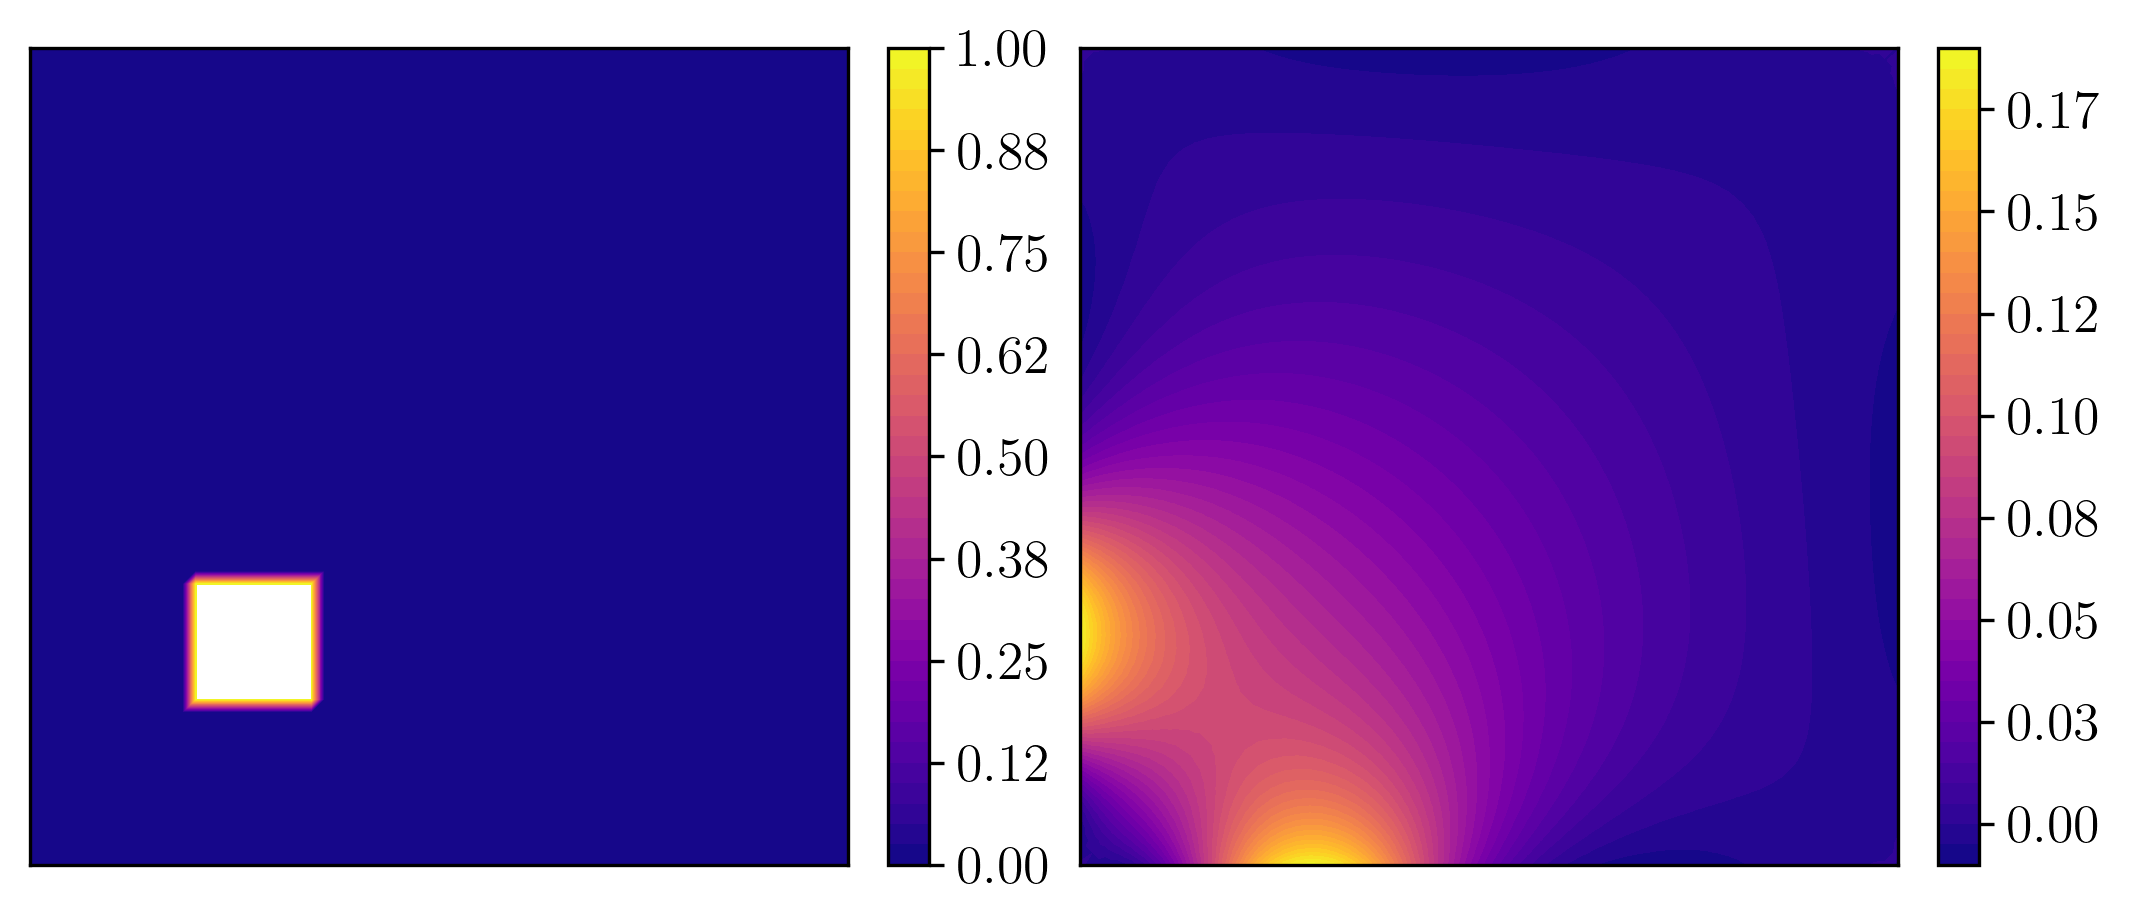
\includegraphics[width=0.75\textwidth]{standard_tikhonov_solution.png}}
    \caption{The true source $x$ (left) and a standard Tikhonov solution $x_\lambda$ (right), where $\lambda = 10^{-4}$.}
    \label{fig:standard_tikhonov_solution}
\end{figure*}
Replacing $\mathcal{K}$ by its discretization $K \in \mathbb{R}^{N_b \times N}$ and the $L^2$ norms by the FEM inner products in Equations~\eqref{eq:fem_norm} and~\eqref{eq:fem_norm_ds}, the Tikhonov problem in Equation~\eqref{eq:problem} takes the discrete form
\begin{equation}\label{eq:discrete_inverse_problem}
    \min_{x \in \mathbb{R}^N}
    \| K x - y \|_{M_\partial}^2
    + \lambda^2 \| W x \|_M^2,
\end{equation}
where $x \in \mathbb{R}^N$ is the coefficient vector of $f_h \in V_h$, $y \in \mathbb{R}^{N_b}$ is the observed boundary data, $\lambda \ge 0$ is the regularization parameter, and $W$ the regularization weight matrix.

Standard Tikhonov ($W = I$) does not work here. Because $K$ has a large null space, the solutions it produces concentrate near the domain boundary regardless of where the true source is located \cite{elvetunRegularizationOperatorSource2020}. This is illustrated in Figure~\ref{fig:standard_tikhonov_solution}.


\subsubsection{Regularization weights}
Assume that $\{ \phi_i \}$ is an orthonormal basis of $V_h$, let $\operatorname{Nul}(\mathcal{K})$ denote the null space of $\mathcal{K}$ and $\operatorname{Nul}(\mathcal{K})^\perp$ its orthogonal complement. Any source $f \in V_h$ can be written as $f = f_\perp + f_0$, where $f_\perp \in \operatorname{Nul}(\mathcal{K})^\perp$ and $f_0 \in \operatorname{Nul}(\mathcal{K})$. As Elvetun and Nielsen point out in \cite{elvetunRegularizationOperatorSource2020}, sources $f$ located near the domain boundary have a larger $f_\perp$ component, and sources deep within the domain have a larger $f_0$ component. If $f^* = \mathcal{K}^+ y$ denotes the least-squares minimum-norm solution, they show that for the case when $f = \phi_j$, we have that
\begin{equation*}
    f^* = \sum_{i} \langle \hat P f, \phi_i \rangle \phi_i,    
\end{equation*}
where $\hat P: V_h \to \operatorname{Nul}(\mathcal{K})^\perp$ is the orthogonal projection onto $\operatorname{Nul}(\mathcal{K})^\perp$. Since $\hat{P}\phi_i = \phi_{i,\perp}$, basis functions deep in the interior have small $\|\hat{P}\phi_i \|$. By the Cauchy-Schwarz inequality, if $\| \hat P \phi_i \|$ is small, then $\langle \hat Pf, \phi_i \rangle$ is small, and the corresponding component of $f^*$ is small. This means that for any $\phi_i$ far away from $\partial \Omega$, the corresponding component of $f^*$ is forced to be small, introducing bias to the solution. This issue transfers to the standard Tikhonov solution $f_\lambda$ since $f_\lambda \to f^*$ as $\lambda \to 0$ \cite{engl1996regularization}.

Elvetun and Nielsen counteract this by re-scaling the norm of $\hat P \phi_i$ such that $\| \hat P \phi_i \| = 1$. This is achieved by setting $w_i = \| \hat P \phi_i \|$ with $W = \operatorname{diag}(w_i)$ in the Tikhonov formulation, equalizing the contribution of all components. In the discrete formulation, $\hat P = K^+ K$ is the orthogonal projection onto the complement of the null space, and the weights are computed as $w_i = \|K^+ K e_i\|$.

In our setting, the basis of the element space $V_h$ given in Equation~\eqref{eq:fem_space} needs to be normalized to match the orthonormality assumption made above. If $K = U\Sigma V^T$ is the SVD of $K$ and $M_{ii}$ is the $i$-th diagonal element of the mass matrix $M$, then the weights are computed as 
\begin{equation}\label{eq:weights}
    w_i =
    \frac{\| K^+ K e_i \|_M}
         {\| \phi_i \|_M} =
    \frac{\| V V^T e_i \|_M}
         {\sqrt{M_{ii}}},
    \quad i = 1, \dots, N,
\end{equation}
and $W = \operatorname{diag}(w_1, \dots, w_N)$.


\subsubsection{A transformed formulation}
The weights in Equation~\eqref{eq:weights} are defined by measuring length in the subspace $\operatorname{Nul}(K)^\perp \subset \mathbb{R}^N$. However, the residual vector $K x - y$ in Equation \eqref{eq:discrete_inverse_problem} is measured in the boundary space $\mathbb{R}^{N_b}$. Following Elvetun and Nielsen in \cite{elvetunWeightedSparsityRegularization2023}, we can reformulate the equation $K x = y$ as the equivalent problem $K^+ K x = K^+ y$ (since $K$ and $K^+K$ share the same nullspace). Now, the residual $K^+ K x - K^+ y$ lives in the subspace $\operatorname{Nul}(K)^\perp$, the same space where the weights $w_i$ are defined. Motivated by this, we replace the original residual by the transformed one, giving
\begin{equation}\label{eq:transformed_discrete_inverse_problem}
    \min_{x \in \mathbb{R}^N}
    \| K^+ K x - K^+ y \|_{M}^2
    + \lambda^2 \| W x \|_M^2.
\end{equation}

In practice, the pseudoinverse $K^+$ amplifies errors associated with small singular values of $K$, and must therefore be approximated by the truncated pseudoinverse $K_k^+$, obtained by keeping the first $k$ singular components in Equation~\eqref{eq:pseudoinverse}. The weights are correspondingly approximated using $P_k = K_k^+ K$.
      % thesis ch. 2
\section{Matrix-free randomized SVD of the forward operator}
\label{sec:rsvd}

% Source: thesis/sections/3_approximating_the_forward_operator.tex
% \section{Approximating the forward operator}\label{sec:approximating}
\begin{figure*}[thbp]
    \centerline{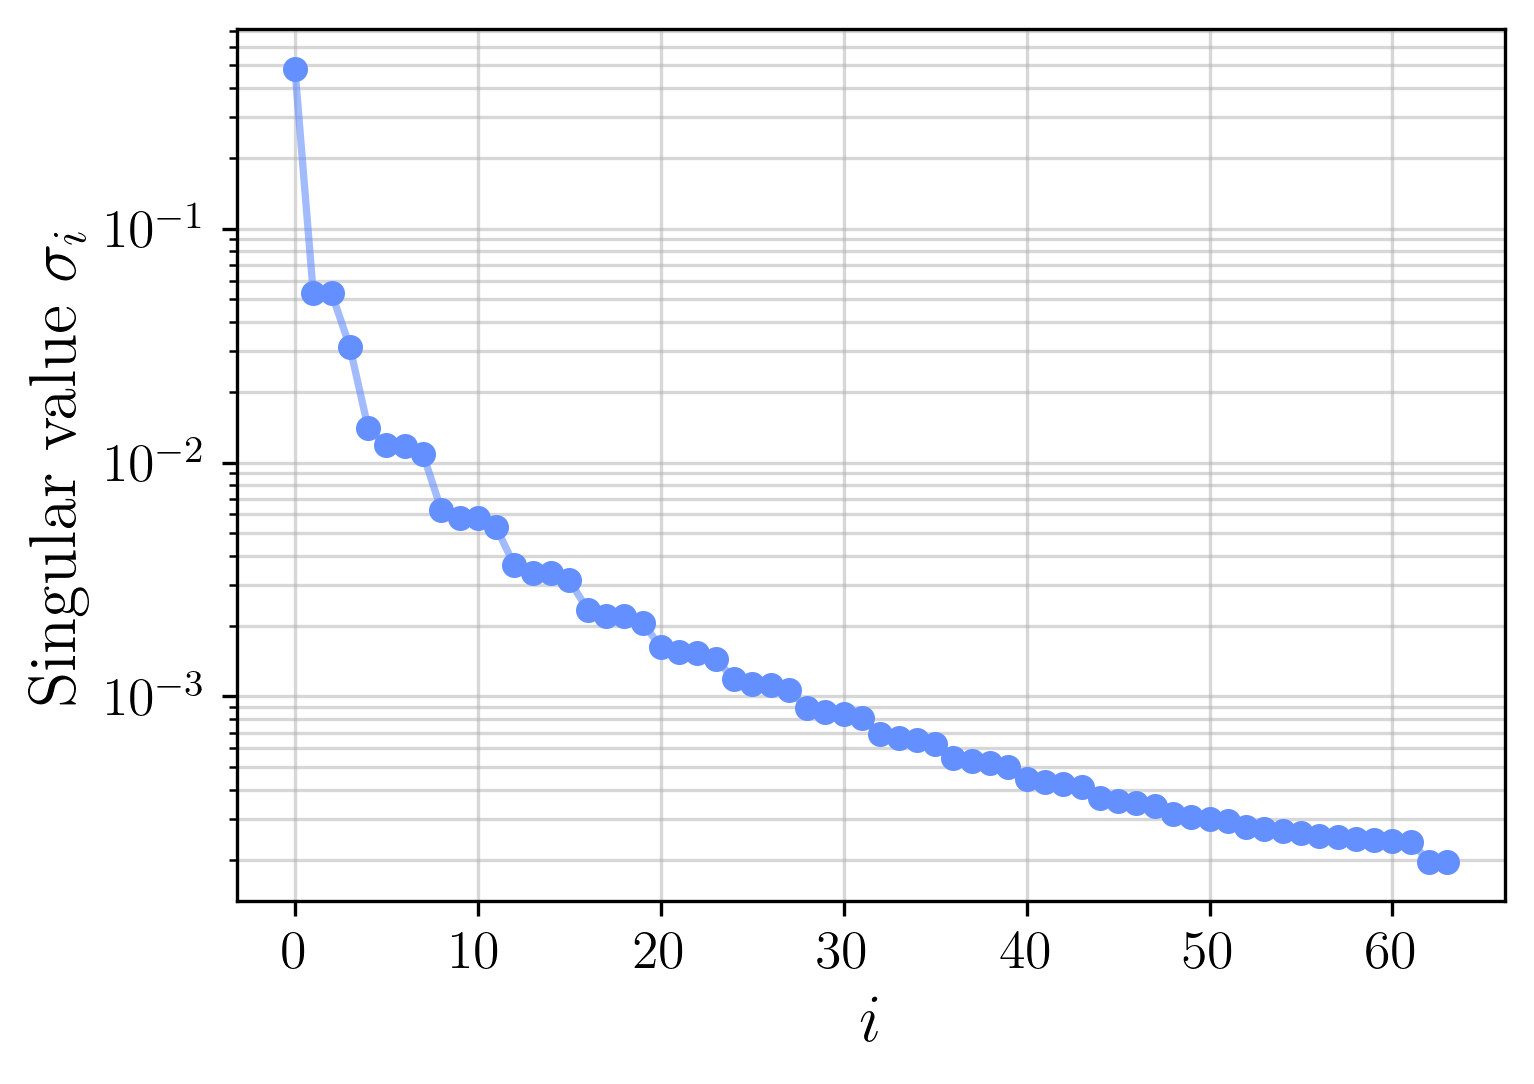
\includegraphics[width=0.6\textwidth]{singular_values.png}}
    \caption{The rapidly decaying singular values $\sigma_1, \dots, \sigma_{64}$ of a $64 \times 289$ matrix $K$ constructed from a $16 \times 16$ rectangular mesh. The y-axis uses a log scale.}
    \label{fig:singular_values}
\end{figure*}
% Opening: motivation and feasibility
The goal of this section is to compute the regularization weights given in Equation \eqref{eq:weights}, which requires the SVD $K = U\Sigma V^T$. Using the identity $K^T = MA_h^{-1}T^T$, $K$ can be formed with $N_b$ linear solves of $A_h v_i = T^T e_i$. With a sparse Cholesky factorization of $A_h$ at cost $\mathcal{O}(N^{3/2})$ and triangular solves at $\mathcal{O}(N \log N)$ in two dimensions (Section~\ref{sec:initial_matrix_factorizations}), forming $K$ takes $\mathcal{O}(N_b N \log N)$. The SVD of the resulting dense $N_b \times N$ matrix then costs $\mathcal{O}(N_b^2 N)$ \cite{dongarraSingularValueDecomposition2018}. Since $N$ grows quadratically with mesh resolution in two dimensions and cubically in three, forming $K$ and computing its SVD is infeasible at fine meshes.

The randomized SVD (Algorithm~\ref{alg:rsvd}) reduces this cost to $\mathcal{O}(l N_b N)$ \cite{halkoFindingStructureRandomness2011}, where $l = k + p$ is a small constant, $k$ is the target rank, and $p$ is an oversampling parameter (typically, $p \in [5, 10]$ \cite{halkoFindingStructureRandomness2011}). It yields a rank-$k$ approximation $K \approx U \Sigma V^T$, and since $K$ has a large nullspace and rapidly decaying singular values, as illustrated in Figure~\ref{fig:singular_values}, $l$ can be chosen much smaller than $N_b$. Unlike $N_b \sim \sqrt{N}$, $l$ can be held constant when the mesh is refined (as shown in Section~\ref{sec:mesh_resolution_effect_on_reconstruction_error}), so the ratio $l / N_b$ shrinks as $N$ increases and the rSVD becomes increasingly advantageous for larger problems.

The rSVD implementation of Algorithm~\ref{alg:rsvd} requires forming $B = Q^T K$, which requires $K$ to be stored as a dense $N_b \times N$ matrix. We instead propose a matrix-free variant without assembling $K$, at a cost of $l$ forward PDE solves and $l$ adjoint PDE solves.


\subsection{A matrix-free rSVD scheme}\label{sec:a_matrix_free_rsvd_scheme}
\begin{figure}[thbp]
    \centering
    \begin{tikzpicture}[
        scale=0.7,
        >=stealth,
        line width=0.9pt,
        every node/.style={font=\large}
    ]
    % Left: unit circle
    \begin{scope}[shift={(0,0)}]
      % circle
      \draw[thick] (0,0) circle (2);
      % dotted guidelines
      \draw[densely dotted] (-2,0) -- (0,0);
      \draw[densely dotted] (0,-2) -- (0,0);
      % e1, e2
      \draw[thick,->] (0,0) -- (2,0) node[right] {$e_1$};
      \draw[thick,->] (0,0) -- (0,2) node[above] {$e_2$};
      % omega, length=2, angle=35
      \draw[thick,->,Green] (0,0) -- ({2*cos(35)},{2*sin(35)}) node[above right] {$\psi$};
    \end{scope}
    
    % Middle: K arrow
    \begin{scope}[shift={(3.5,0)}]
      \draw[very thick,->]
        (-1,0.8) to[out=40, in=140] (1.4,0.8);
      \node[above] at (0.2,1.25) {$K$};
    \end{scope}
    
    % Right: ellipse + vectors
    \begin{scope}[shift={(8,0)}, rotate=25]
      % ellipse
      \draw[thick] (0,0) ellipse (3.5 and 1.5);
      % dotted principal axes
      \draw[densely dotted] (-3.5,0) -- (3.5,0);
      \draw[densely dotted] (0,-1.5) -- (0,1.5);
      % u1 and u2
      \draw[thick,->] (0,0) -- (3.5,0)
        node[midway, below] {$\sigma_1$}
        node[right] {$u_1$};
      \draw[thick,->] (0,0) -- (0,1.5)
        node[midway, left] {$\sigma_2$}
        node[above] {$u_2$};
      % omega
      \draw[thick,->,Green] (0,0) -- (3.2,0.6)
      node[above, xshift=5pt, yshift=2pt] {$K \psi$};
    \end{scope}
    \end{tikzpicture}
    \caption{The geometry of the rSVD: A random sample $K\psi$ aligns mostly with the dominant left singular vectors of $K$. The illustration is inspired by Figure~9.1 in Tropp \cite{troppACM204Randomized2021}.}
    \label{fig:rsvd}
\end{figure}
The algorithm consists of two stages. The first stage constructs an approximate basis $Q$ for the column space of $K$. We select a target rank $k$ and an oversampling parameter $p$, set $l = k + p$, and apply $K$ to $l$ random test vectors $\psi_1, \psi_2, \dots, \psi_l$ drawn from a distribution of choice, typically the standard normal distribution \cite{halkoFindingStructureRandomness2011}. This yields $l$ random samples $y_1, y_2, \dots, y_l$, where $y_i = K \psi_i$. Collecting these into matrices $Y = [y_i]_{i=1}^l$ and $\Psi = [\psi_i]_{i=1}^l$, we have
\begin{equation*}
    Y = K \Psi.
\end{equation*}
Each sample $K\psi_i$ is a linear combination of the columns of $K$, and tends to align with the dominant left singular vectors, see Figure~\ref{fig:rsvd}. Orthogonalizing the columns of $Y$ via a QR-factorization $QR = Y$ ensures that $\operatorname{span}\{q_1, \ldots, q_l\}$ approximately aligns with $\operatorname{span}\{u_1, \ldots, u_l\}$, giving
\begin{equation*}
    \operatorname{range}(Q) \approx \operatorname{range}(K).
\end{equation*}

The second stage projects $K$ onto $\operatorname{range}(Q)$ by computing $B = Q^T K$. Since we do not know $K$ explicitly, we use $K^*$ to compute $B$. In particular, by the definition of $K^*$,
\begin{equation}\label{eq:K_star}
    (K^* z)^T M = z^T M_\partial K.
\end{equation}
If we choose $z = M_{\partial}^{-1} q_i$ and insert it into Equation~\eqref{eq:K_star}, we see that
\begin{equation}\label{eq:rsvd_relation}
    (K^* z)^T M
    = (M_{\partial}^{-1} q_i)^T M_{\partial} K
    = q_i^T K.
\end{equation}
Setting $b_i = (K^* (M_{\partial}^{-1} q_i))^T M$ for $i = 1, 2, \dots, l$, and defining the $l \times N$ matrix
\begin{equation*}
    B = \begin{bmatrix} b_1 \\ \vdots \\ b_l \end{bmatrix},
\end{equation*}
we obtain, by Equation~\eqref{eq:rsvd_relation},
\begin{equation*}
    B = Q^T K.
\end{equation*}
Taking the SVD $B = \tilde U \Sigma V^T$, and setting $U = Q \tilde U$, gives an approximate SVD
\begin{equation}\label{eq:rsvd_approx}
    K \approx U \Sigma V^T.
\end{equation}

The factorization in \eqref{eq:rsvd_approx} is of rank $l$, since $U \Sigma V^T = Q \tilde U \Sigma V^T = Q B = Q Q^T K$ with $\operatorname{rank}(Q) = l$. A rank-$k$ factorization is obtained by selecting the $k$ first columns of the respective matrices in \eqref{eq:rsvd_approx}. The procedure is summarized in Algorithm~\ref{alg:discrete_rsvd}.
\begin{algorithm}[!thbp]
\caption{Matrix-free rSVD approximation of $K$}
\label{alg:discrete_rsvd}
\begin{algorithmic}[1]
    \Require Forward operator $K: \mathbb{R}^N \to \mathbb{R}^{N_b}$, adjoint operator $K^*: \mathbb{R}^{N_b} \to \mathbb{R}^N$, mass matrices $M, M_\partial$, target rank $k$, oversampling parameter $p$
    \Ensure Approximate rank-$k$ factorization $K \approx U \Sigma V^T$
    
    \State \textbf{Range sketch:}
    \State Set $l = k + p$
    \Comment{Ensure that $l \le N_b$}
    \For{$i = 1, \dots, l$}
        \State Draw a random vector $\psi_i \in \mathbb{R}^N$
        \State Apply the forward operator: $y_i = K \psi_i \in \mathbb{R}^{N_b}$
    \EndFor

    \State Form the matrix $Y = [y_1, \dots, y_l] \in \mathbb{R}^{N_b \times l}$ \Comment{Equivalent to $Y = K \Psi$}
    \State Compute an orthonormal basis: $Q = \operatorname{orth}(Y)$

    \State \textbf{Projection onto the basis:}
    \For{$i = 1, \dots, l$}
        \State Let $q_i$ be the $i$-th column of $Q$
        \State Solve for $\tilde q_i = M_{\partial}^{-1} q_i$
        \State Apply the adjoint operator: $\tilde b_i = K^* \tilde q_i$
        \State Set $b_i = \tilde b_i^T M$ \Comment{$i$-th row of $B$}
    \EndFor
    \State Form the projected matrix $B = \begin{bmatrix} b_1 \\ \vdots \\ b_l \end{bmatrix} \in \mathbb{R}^{l \times N}$
    \Comment{Equivalent to $B = Q^T K$}

    \State Compute the SVD: $B = \tilde U \Sigma V^T$
    \State Set $U = Q \tilde U$
    \State Truncate to rank $k$: $U, \Sigma, V^T \leftarrow \operatorname{truncate}_k(U, \Sigma, V^T)$
    
\end{algorithmic}
\end{algorithm}


\subsection{Initial matrix factorizations}\label{sec:initial_matrix_factorizations}
Algorithm~\ref{alg:discrete_rsvd} factorizes the stiffness matrix $A_h$ and the boundary mass matrix $M_\partial$ once at initialization. Each application of $K$ or $K^*$ then reduces to sparse matrix products and triangular solves with $A_h$, and each mass matrix solve $M_\partial \tilde{q}_i = q_i$ reduces to triangular solves with the factorization of $M_\partial$.

Under the assumptions that $\sigma$ is positive (symmetric positive definite in the matrix-valued case) and $c > 0$, the matrix $A_h$ is SPD. The boundary mass matrix $M_\partial$ is also SPD \cite{larsonFiniteElementMethod2013}. These matrices can therefore be factorized using the Cholesky decomposition. The sparse structure of the stiffness and mass matrices can be exploited to efficiently compute such factorizations. For instance, the nested dissection method, proposed by George \cite{georgeNestedDissectionRegular1973}, may compute such a Cholesky factorization in $\mathcal{O}(N^{3/2})$ computations. In two dimensions, nested dissection gives a Cholesky factor $L$ with $\mathcal{O}(N \log N)$ nonzero entries. Sparse triangular solves cost $\mathcal{O}(\operatorname{nnz}(L))$, where $\operatorname{nnz}(L)$ denotes the number of nonzero entries in $L$. Thus, after factorization, each solve costs $\mathcal{O}(N \log N)$ \cite{georgeComputerSolutionLarge1984,liptonGeneralizedNestedDissection1979}.

In particular, if $A_h = LL^T$ is a Cholesky factorization, then $K = T (LL^T)^{-1}M$. To compute $y_i = K \psi_i$, the system $LL^T v = M \psi_i$ is solved via two triangular solves, and $y_i = T v$. A similar procedure is done when applying $K^* = A_h^{-1}T^TM_\partial$, where the factorization $A_h = LL^T$ can be reused since $A_h = A_h^T$.
               % thesis ch. 3
\section{Dynamical low-rank approximation with conjugate directions}
\label{sec:dlracg}

% Source: thesis/sections/4_dynamical_low_rank_solver.tex
% \section{Dynamical low-rank approximation}\label{sec:dynamical_low_rank_approximation}
\begin{figure*}[thbp]
    \centerline{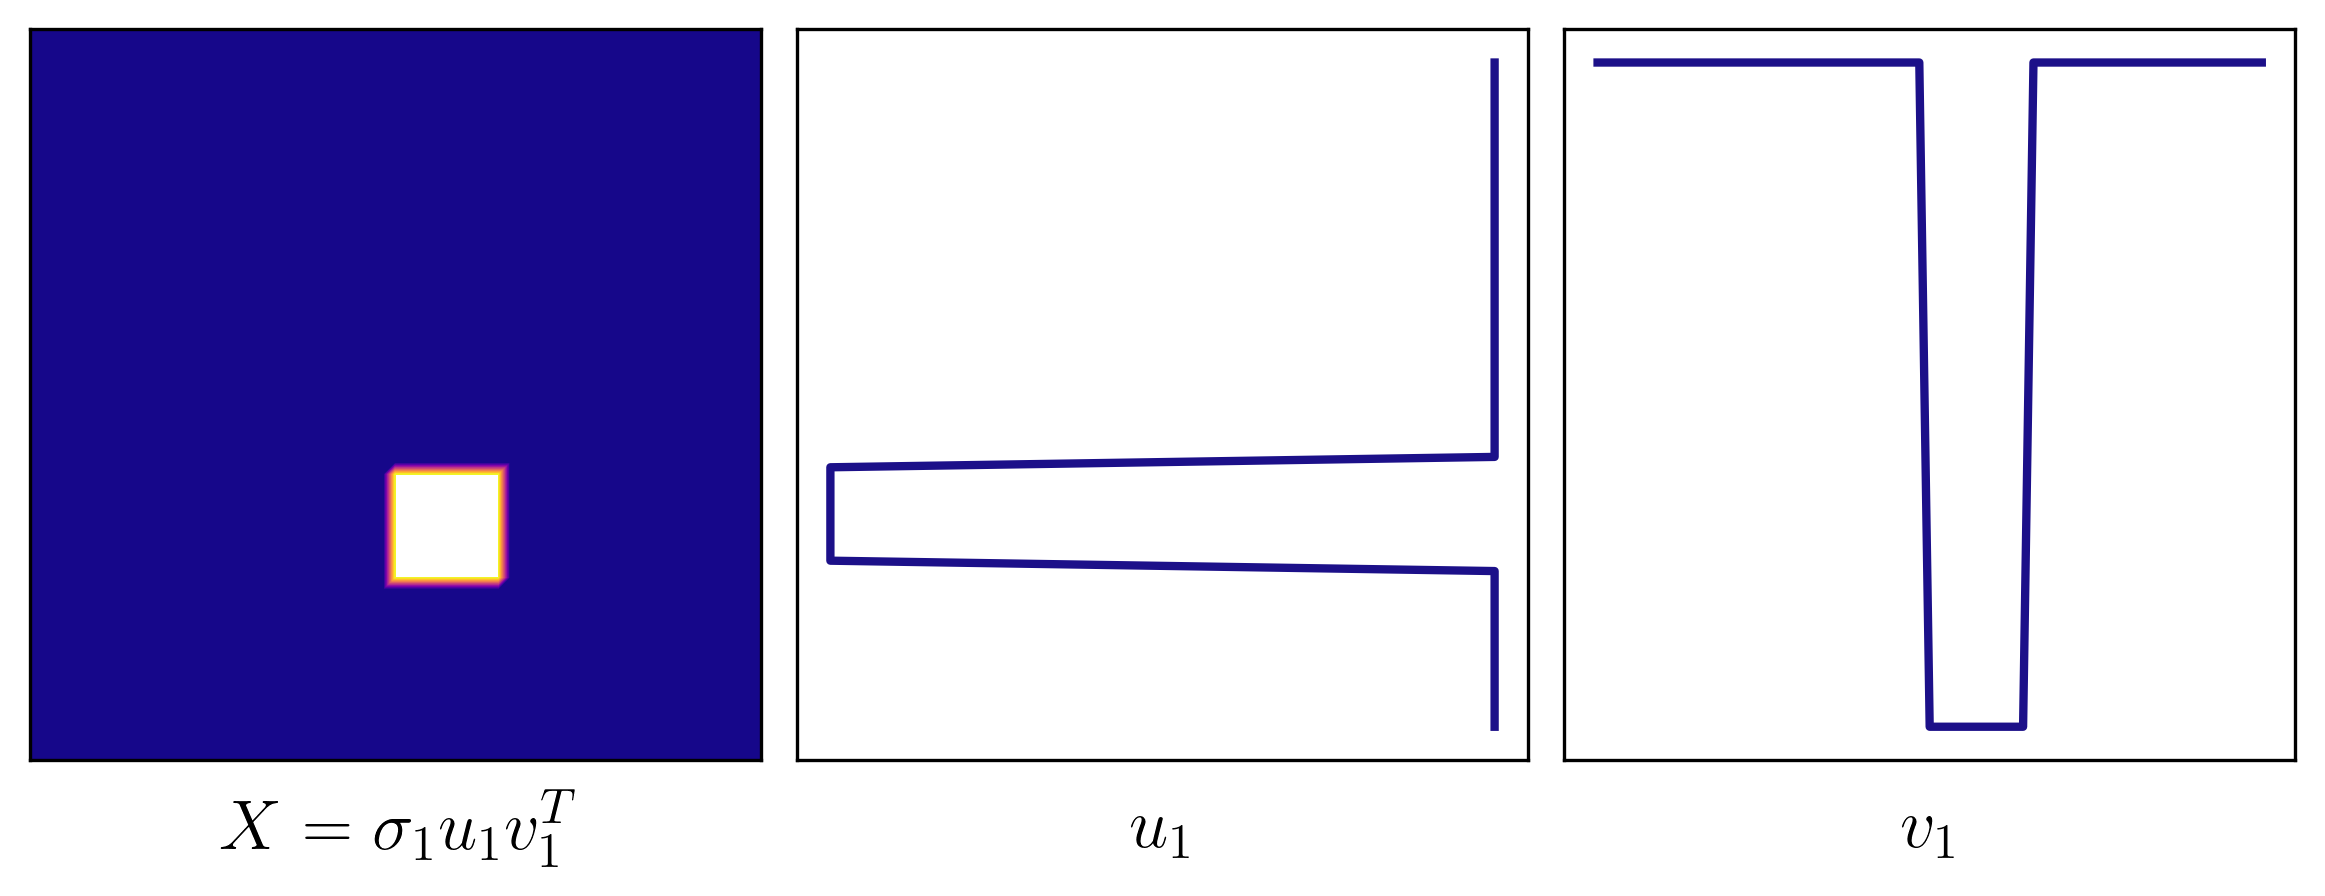
\includegraphics[width=1.0\textwidth]{low_rank_source.png}}
    \caption{Rank-1 outer product representation of a single square source (left), $X = \sigma_1 u_1 v_1^T$. The left singular vector $u_1$ (middle) is plotted along the vertical axis, and the right singular vector $v_1$ (right) along the horizontal axis.}
    \label{fig:low_rank_source}
\end{figure*}
In many applications, the source $f \in L^2(\Omega)$ in Equation~\eqref{eq:problem} is sparse \cite{elvetunWeightedSparsityRegularization2023}, and often well-approximated by low-rank matrices. If $x \in \mathbb{R}^{n^2}$ is a discretization of $f$ and $X = \operatorname{mat}(x)$ is its reordering into an $n \times n$ matrix, we can often expect $r = \operatorname{rank}(X) \ll n$. The SVD writes $X$ as a sum of $r$ outer products,
\begin{equation*}
    X = \sum_{i=1}^{r} \sigma_i u_i v_i^T,
\end{equation*}
each parameterized by two vectors $u_i, v_i \in \mathbb{R}^n$ (Figure~\ref{fig:low_rank_source}), with $r$ roughly tracking the number of distinct localized sources. Since the source itself is low-rank, we restrict the search to rank-$r$ matrices, working directly with the factors $u_i, v_i$ rather than the full 
matrix $X$.


\subsection{The low-rank manifold}
\begin{figure*}[thbp]
    \centerline{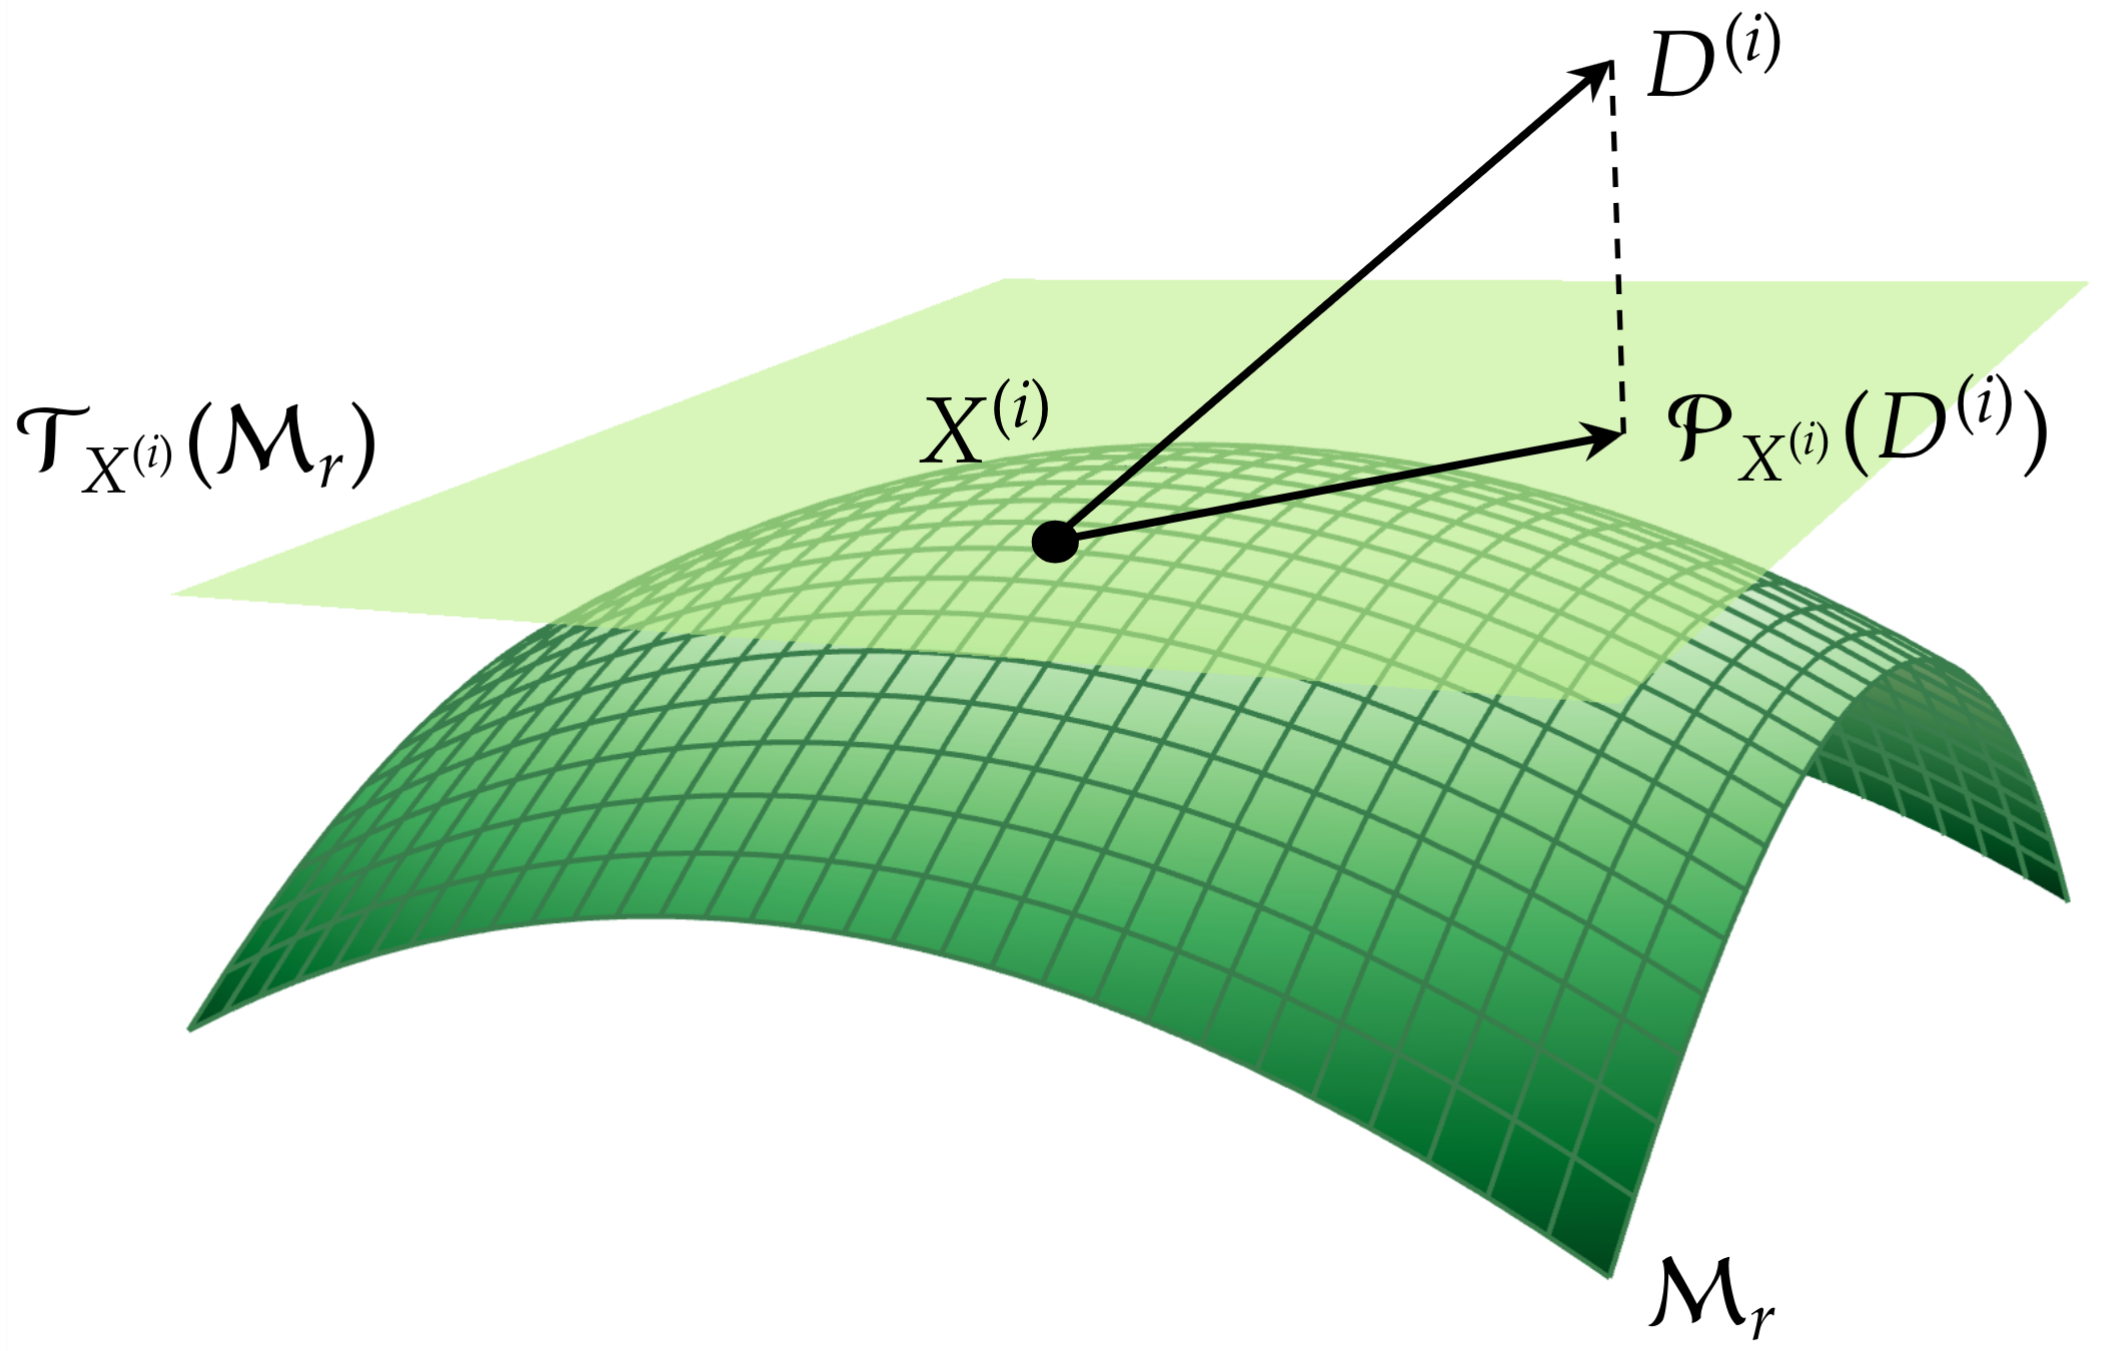
\includegraphics[width=0.6\textwidth]{low_rank_manifold.png}}
    \caption{Illustration of the DLRA algorithm: the point $X^{(i)}$ lies on the manifold of rank-$r$ matrices $\mathcal{M}_r$, and $D^{(i)}$ is projected onto the tangent plane $\mathcal{T}_{X^{(i)}}(\mathcal{M}_r)$.}
    \label{fig:low_rank_manifold}
\end{figure*}
Consider the problem of finding a rank-$r$ solution $X$ via the update scheme $X^{(i+1)} = X^{(i)} + \alpha_i D^{(i)}$, where $D^{(i)}$ is a search direction and $\alpha_i > 0$ a step size. Starting from a rank-$r$ matrix $X^{(0)}$, there is in general no guarantee that $D^{(i)}$ preserves low rank, so that $X^{(i)}$ may leave the space $\mathcal{M}_r$ of rank-$r$ matrices after a single step.

One can replace $D^{(i)}$ by its projection onto the tangent space $\mathcal{T}_{X^{(i)}}(\mathcal{M}_r)$, a classical concept from Riemannian geometry \cite{docarmoRiemannianGeometry1992,absilOptimizationAlgorithmsMatrix2008}. This is the idea behind the Dynamical Low-Rank Approximation (DLRA) of Koch and Lubich \cite{kochDynamicalLowrankApproximation2007}. They proposed, in a continuous-time setting, evolving an approximation on $\mathcal{M}_r$ by projecting the derivative of the matrix onto the tangent space at the current approximation. Using this concept in our discrete setting, we replace $D^{(i)}$ by its tangent-space projection $\mathcal{P}_{X^{(i)}}(D^{(i)})$, yielding the update
\begin{equation*}
    X^{(i+1)} = X^{(i)} 
    + \alpha_i \mathcal{P}_{X^{(i)}}(D^{(i)}).
\end{equation*}
This is illustrated in Figure~\ref{fig:low_rank_manifold}. Rather than updating $X^{(i)}$ directly, the DLRA algorithm operates on a factorization $X^{(i)} = U_x \Sigma_x V_x^T$, where $U_x$ and $V_x$ have orthonormal columns and $\Sigma_x$ is non-singular (and diagonal if using the SVD), updating the factors at each iteration. We use the subscript ``$x$'' to distinguish these factors from those of the forward operator $K = U \Sigma V^T$.

However, as pointed out by Koch and Lubich, when $\Sigma_x$ is ill-conditioned, which occurs when $r$ exceeds the effective rank of $X^{(i)}$, the projector $\mathcal{P}_{X^{(i)}}$ suffers from stiffness, leading to very small step sizes and issues with rounding errors.

To address this, Lubich and Oseledets proposed splitting the projector $\mathcal{P}_{X^{(i)}}$ into simpler sub-projections \cite{lubichProjectorsplittingIntegratorDynamical2013}. Crucially, each sub-projection can be evaluated without forming $\Sigma_x^{-1}$, and avoids the stiffness problem present in the original formulation \cite{kieriDiscretizedDynamicalLowrank2016}. In recent years, additional advancements have been made to DLRA, offering improved stability \cite{kuschStabilityRobustDynamical2023a}, parallelism \cite{cerutiParallelRankadaptiveIntegrator2024}, and rank-adaptivity \cite{cerutiRankadaptiveRobustIntegrator2021}.

Schotthöfer et al.\ \cite{schotthoferLowrankLotteryTickets2022} recently proposed a discrete rank-adaptive update scheme based on the ``unconventional'' basis update and Galerkin step integrator \cite{cerutiUnconventionalRobustIntegrator2020} for training low-rank neural networks, see Algorithm~\ref{alg:dlra}. The discrete DLRA scheme used in this paper follows their formulation.
\begin{algorithm}
\caption{Schotthöfer et al.'s DLRA scheme}
\label{alg:dlra}
\begin{algorithmic}[1]

\Require Initial matrix $X^{(0)}$ with SVD $X^{(0)} = U_x \Sigma_x V_x^T$, solution rank $r$, step-size rule $\{\alpha_i\}$

\Ensure Rank-$r$ solution $x = \operatorname{vec}(X)$

\For{$i = 0,1,2,\dots,\text{max\_iter}$}

    \State \textbf{Search direction:}
    \State $D^{(i)} = -\nabla \Phi(X^{(i)})$

    \State \textbf{Dynamical low-rank update (KLS step):}
    \State $K' = U_x \Sigma_x + \alpha_i D^{(i)} V_x$
    \State $L' = V_x \Sigma_x^T + \alpha_i (D^{(i)})^T U_x$
    \State $\hat U = \operatorname{orth}([U_x, K'])$
    \State $\hat V = \operatorname{orth}([V_x, L'])$
    \State $\hat \Sigma = (\hat U^T U_x)\Sigma_x(V_x^T \hat V) + \alpha_i (\hat U^T D^{(i)} \hat V)$
    \State $(U_x, \Sigma_x, V_x) = \operatorname{truncate}_r(\hat U, \hat \Sigma, \hat V)$
    \Comment{$X^{(i+1)} = U_x \Sigma_x V_x^T$}

\EndFor

\end{algorithmic}
\end{algorithm}

\subsection{Step-size selection and rank adaptation}
Algorithm~\ref{alg:dlra} admits several choices for the step size $\alpha_i$ and the truncation criterion.

\paragraph{Step size.}
We consider three step-size rules. A fixed step size $\alpha_i = \alpha > 0$ coincides with one step of gradient descent on the factors $K'$, $L'$, and
$\hat \Sigma$, analogous to the stochastic gradient descent (SGD) step used by Schotthöfer et al. \cite{schotthoferLowrankLotteryTickets2022}, but using the full gradient. Adam computes adaptive step sizes from estimates of the first and second moments of the gradient \cite{kingmaAdamMethodStochastic2017}, and Schotthöfer et al. find it converges faster in practice than SGD for training neural networks \cite{schotthoferLowrankLotteryTickets2022}. More recently, they showed that classical momentum methods like Adam can struggle due to the geometry of $\mathcal{M}_r$ \cite{schotthoferGeometricFrameworkMomentumbased2025}.

For the quadratic objective $\Phi$ considered in this paper (Equation~\eqref{eq:discrete_inverse_problem}), steepest descent selects the step size that minimizes $\Phi$ along $D^{(i)} = -\nabla \Phi(X^{(i)})$,
\begin{equation*}
    \alpha_i = \frac{\|\nabla\Phi(X^{(i)})\|_F^2}
                    {\langle D^{(i)},\, H D^{(i)} \rangle_F},
\end{equation*}
and requires no tuning (Section~8.2 in Chong et al.\ 
\cite{chong2023introduction}).

\paragraph{Rank adaptation.} In the dynamical low-rank update (KLS) step of Algorithm~\ref{alg:dlra}, the factors $\hat{U}$ and $\hat{V}$ have $2r$ columns and $\hat{\Sigma}$ is of shape $2r \times 2r$. The truncation step (line 10) moves the factors back to a specified maximum rank $r$ \cite{schotthoferLowrankLotteryTickets2022}. The truncation can also be done adaptively via a truncation threshold $\vartheta$, as done by Schotthöfer et al.\ \cite{schotthoferLowrankLotteryTickets2022}. 


\subsection{Application to the inverse problem}\label{sec:application_to_inverse_problem}
In the following sections, we consider the problem of minimizing a quadratic objective function
\begin{equation*}
    \Phi: \mathbb{R}^{n \times n} \rightarrow \mathbb R.
\end{equation*}
In our discrete case, the minimization problem given in Equation~\eqref{eq:discrete_inverse_problem} translates into minimizing
\begin{equation*}
    \Phi(X) = \frac 1 2 \|Kx - y\|_{M_\partial}^2
    + \frac{\lambda^2}{2} \| W x \|_M^2.
\end{equation*}
Using the product rule, we get the gradient $\nabla \Phi$ and Hessian $H$ of $\Phi$ with respect to $x$,
\begin{equation*}
    \begin{aligned}
    \nabla \Phi (X) &= K^T M_\partial (K x - y) + \lambda^2 W^T M W x, \\
    H &= K^T M_\partial K + \lambda^2 W^T M W.
    \end{aligned}
\end{equation*}
The Hessian is SPD, since $K^T M_\partial K$ is positive semidefinite, $\lambda^2 W^T M W$ is positive definite, and their sum is therefore positive definite. By the optimality condition $\nabla \Phi (X) = 0$, the minimizer of $\Phi$ is the solution of $H x = K^T M_\partial y$, i.e.,~the normal equations of Equation~\eqref{eq:discrete_inverse_problem}.


\subsection{DLRA with conjugate search directions}
Since $\Phi$ is quadratic with an SPD Hessian $H$, the conjugate gradient (CG) method is a natural minimization strategy \cite{saadIterativeMethodsSparse2003,fletcherFunctionMinimizationConjugate1964,hestenesMethodsConjugateGradients1952}.

CG generates a sequence of search directions $\{D^{(i)}\}$ that are $H$-conjugate, i.e., $\langle D^{(i)}, H D^{(j)}\rangle_F = 0$ for $i \neq j$. Starting from the initial search direction $D^{(0)} = -G^{(0)}$, each step computes an optimal step size
\begin{equation*}
    \alpha_i = \frac{\|G^{(i)}\|_F^2}{\langle D^{(i)},\, H D^{(i)}\rangle_F},
\end{equation*}
and updates the search direction by the Fletcher-Reeves rule \cite{fletcherFunctionMinimizationConjugate1964},
\begin{equation}\label{eq:fletcher-reeves}
    D^{(i+1)} = -G^{(i+1)} + \beta_i D^{(i)},
    \qquad
    \beta_i = \frac{\|G^{(i+1)}\|_F^2}{\|G^{(i)}\|_F^2}.
\end{equation}

In our low-rank setting, we propose replacing the descent directions used in the method of Schotthöfer et al. (Algorithm~\ref{alg:dlra}) with $H$-conjugate search directions $\{D^{(i)}\}$ obtained via the CG method. The motivation is that $H$-conjugate directions exploit curvature information of $H$, leading to faster convergence. The full scheme is given in Algorithm~\ref{alg:DLRA-CG}, which we refer to as DLRA-CG throughout.
\begin{algorithm}
\caption{DLRA-CG scheme}
\label{alg:DLRA-CG}
\begin{algorithmic}[1]

\Require Hessian $H$, initial matrix $X^{(0)}$ with SVD $X^{(0)} = U_x \Sigma_x V_x^T$, solution rank $r$

\Ensure Rank-$r$ solution $x = \operatorname{vec}(X)$

\State Compute initial gradient $G^{(0)} = \nabla \Phi(X^{(0)})$
\State Set initial search direction $D^{(0)} = -G^{(0)}$

\For{$i = 0,1,2,\dots,\text{max\_iter}$}

    \State \textbf{Step size:}
    \State $\displaystyle \alpha_i = \frac{\|G^{(i)}\|_F^2}{\langle D^{(i)}, H D^{(i)} \rangle_F}$
    \Comment{$HD^{(i)} = \operatorname{mat}[H \operatorname{vec}(D^{(i)})]$}

    \State \textbf{Dynamical low-rank update (KLS step):}
    \State $K' = U_x \Sigma_x + \alpha_i D^{(i)} V_x$
    \State $L' = V_x \Sigma_x^T + \alpha_i (D^{(i)})^T U_x$
    \State $\hat U = \operatorname{orth}([U_x, K'])$
    \State $\hat V = \operatorname{orth}([V_x, L'])$
    \State $\hat \Sigma = (\hat U^T U_x)\Sigma_x(V_x^T \hat V) + \alpha_i (\hat U^T D^{(i)} \hat V)$
    \State $(U_x, \Sigma_x, V_x) = \operatorname{truncate}_r(\hat U, \hat \Sigma, \hat V)$
    \Comment{$X^{(i+1)} = U_x \Sigma_x V_x^T$}

    \State \textbf{Search direction update:}
    \State $G^{(i+1)} = G^{(i)} + \alpha_i H D^{(i)}$ 
    %\Comment{or $G^{(i+1)} = \nabla \Phi(X^{(i)})$}
    \State $\displaystyle \beta_i =
    \frac{\| G^{(i+1)} \|^2_F}
         {\| G^{(i)} \|^2_F}$
    %\Comment{or $\displaystyle \beta_i =
    %\frac{\langle G^{(i+1)}, H G^{(i)} \rangle_F}
    %     {\langle G^{(i)}, H G^{(i)} \rangle_F}$}
    \State $D^{(i+1)} = -G^{(i+1)} + \beta_i D^{(i)}$

\EndFor

\end{algorithmic}
\end{algorithm}


\subsubsection{Restarted CG}\label{sec:restarted_cg}
In Algorithm~\ref{alg:DLRA-CG}, the sequence $\{D^{(i)}\}$ is generated 
independently of the manifold iterates $X^{(i)}$. After the first step, $G^{(i)}$ no longer equals $\nabla\Phi(X^{(i)})$: the recurrence $G^{(i+1)} = G^{(i)} + \alpha_i HD^{(i)}$ tracks the gradient along the full-rank trajectory
\begin{equation}\label{eq:full_rank_iterate}
    Y^{(i)} = X^{(0)} + \sum_{j<i} \alpha_j D^{(j)},
\end{equation}
not along the manifold iterates. As $Y^{(i)}$ and $X^{(i)}$ drift apart, 
$G^{(i)} = \nabla\Phi(Y^{(i)}) \to 0$ as plain CG converges along $Y^{(i)}$, so $\alpha_i \to 0$ and $X^{(i)}$ may stall at a sub-optimal solution.

Restarted CG \cite{powellRestartProceduresConjugate1977} re-computes the true gradient $G^{(i)} = \nabla\Phi(X^{(i)})$ and resets the search direction to $D^{(i)} = -G^{(i)}$ every $N_r$ iterations, discarding the previous search directions. This was originally proposed as a method to counteract the loss of $H$-conjugacy in the construction of $\{D^{(i)}\}$ because of numerical round-off errors \cite{hestenesMethodsConjugateGradients1952, powellRestartProceduresConjugate1977}. In the DLRA-CG setting, restart serves a second purpose beyond correcting round-off: it resets the full-rank trajectory to $Y^{(i)} = X^{(i)}$, restoring $G^{(i)} = \nabla\Phi(X^{(i)})$ and giving the CG recurrence a fresh start from the true iterate position $X^{(i)}$.

In Algorithm~\ref{alg:DLRA-CG}, this replaces the recurrence $G^{(i+1)} = G^{(i)} + \alpha_i HD^{(i)}$ with a fresh gradient evaluation $G^{(i+1)} = \nabla\Phi(X^{(i+1)})$, and sets $D^{(i+1)} = -G^{(i+1)}$, skipping the $\beta_i$ step.


\subsection{DLRA using preconditioned CG}
Preconditioning is a standard technique for accelerating CG methods, referred to as preconditioned CG (PCG). The system $H x = K^T M_\partial y$ is replaced by the equivalent system $P^{-1} H x = P^{-1} K^T M_\partial y$, where $P \approx H$ is the preconditioner matrix. The convergence of CG depends on $\kappa(H)$ (see Section~6.11.3 in Saad \cite{saadIterativeMethodsSparse2003}), so $P$ is chosen such that $\kappa(P^{-1} H) \ll \kappa(H)$. For elliptic PDE-based forward operators $K$, the Hessian $H = K^T M_\partial K + \lambda^2 W^T M W$ typically has a large condition number, making preconditioning effective.

In the DLRA-CG scheme, the preconditioned system $P^{-1} H x = P^{-1} K^T M_\partial y$ leads to the following adjustments in Algorithm \ref{alg:DLRA-CG}:
\begin{equation*}
    \alpha_i = \frac
    {\langle G^{(i)}, Z^{(i)} \rangle_F}
    {\langle D^{(i)}, H D^{(i)} \rangle_F}, \quad
    \beta_i = \frac
    {\langle G^{(i+1)}, Z^{(i+1)} \rangle_F}
    {\langle G^{(i)}, Z^{(i)} \rangle_F}, \quad
    D^{(i+1)} = -Z^{(i+1)} + \beta_i D^{(i)},
\end{equation*}
with $Z^{(i)} = P^{-1} G^{(i)}$. These modifications are equivalent to standard preconditioned conjugate gradient, as originally described by Concus et al. \cite{concusGeneralizedConjugateGradient1976}. The resulting scheme is summarized in Algorithm \ref{alg:DLRA-PCG}, which we refer to as DLRA-PCG.
\begin{algorithm}
\caption{DLRA-PCG scheme}
\label{alg:DLRA-PCG}
\begin{algorithmic}[1]

\Require Hessian $H$, initial matrix $X^{(0)}$ with SVD $X^{(0)} = U_x \Sigma_x V_x^T$, solution rank $r$, preconditioner $P^{-1}$

\Ensure Rank-$r$ solution $x = \operatorname{vec}(X)$

\State Compute initial gradient $G^{(0)} = \nabla \Phi(X^{(0)})$
\State Precondition $Z^{(0)} = P^{-1} G^{(0)}$
\Comment $P^{-1} G^{(0)} =
\operatorname{mat}[P^{-1} \operatorname{vec}(G^{(0)})]$
\State Set initial search direction $D^{(0)} = -Z^{(0)}$

\For{$i = 0,1,2,\dots,\text{max\_iter}$}

    \State \textbf{Step size:}
    \State $\displaystyle \alpha_i =
    \frac{\langle G^{(i)}, Z^{(i)} \rangle_F}
         {\langle D^{(i)}, H D^{(i)} \rangle_F}$
    \Comment{$HD^{(i)} = \operatorname{mat}[H \operatorname{vec}(D^{(i)})]$}

    \State \textbf{Dynamical low-rank update (KLS step):}
    \State $K' = U_x \Sigma_x + \alpha_i D^{(i)} V_x$
    \State $L' = V_x \Sigma_x^T + \alpha_i (D^{(i)})^T U_x$
    \State $\hat U = \operatorname{orth}([U_x, K'])$
    \State $\hat V = \operatorname{orth}([V_x, L'])$
    \State $\hat \Sigma = (\hat U^T U_x)\Sigma_x(V_x^T \hat V) + \alpha_i (\hat U^T D^{(i)} \hat V)$
    \State $(U_x, \Sigma_x, V_x) = \operatorname{truncate}_r(\hat U, \hat \Sigma, \hat V)$
    \Comment{$X^{(i+1)} = U_x \Sigma_x V_x^T$}

    \State \textbf{Search direction update:}
    \State $G^{(i+1)} = G^{(i)} + \alpha_i H D^{(i)}$
    %\Comment{or $G^{(i+1)} = \nabla \Phi(X^{(i)})$ }
    \State $Z^{(i+1)} = P^{-1} G^{(i+1)}$
    \State $\displaystyle \beta_i =
    \frac{\langle G^{(i+1)}, Z^{(i+1)} \rangle_F}
         {\langle G^{(i)}, Z^{(i)} \rangle_F}$
    %\Comment{or $\displaystyle \beta_i =
    %\frac{\langle G^{(i+1)}, H Z^{(i)} \rangle_F}
    %     {\langle G^{(i)}, H Z^{(i)} \rangle_F}$}
    \State $D^{(i+1)} = -Z^{(i+1)} + \beta_i D^{(i)}$

\EndFor

\end{algorithmic}
\end{algorithm}



\subsubsection{Choice of preconditioner}\label{sec:choice_of_preconditioner}
The effectiveness of PCG depends on the choice of $P$. A good preconditioner must approximate $H$ well, but must be cheap to apply at each iteration. We consider four preconditioners: Jacobi scaling, incomplete Cholesky (IC), IC with a Woodbury correction, and a ``perfect'' preconditioner based on a sparse Cholesky factorization.

\paragraph{Jacobi scaling.} A Jacobi preconditioner $P = \operatorname{diag}(H)$ approximates $H$ by its diagonal (Section~11.5, \cite{golubMatrixComputations4th2013}). The approximation is cheap to compute, as $P^{-1}$ is the inverse of a diagonal matrix. It is most effective when $H$ is diagonally dominant.
 
\paragraph{Incomplete Cholesky.} Under the assumption that $K$ is of rank $k$ (for example, obtained using Algorithm~\ref{alg:discrete_rsvd}), the Hessian consists of a low-rank plus a sparse term,
\begin{equation*}
    H = \underbrace{K^T M_\partial K}_{\text{low-rank}}
    + \underbrace{\lambda^2 W^T M W}_{\text{sparse}}
    = F + S.
\end{equation*}
To see why, insert the rank-$k$ SVD of $K$ into $F = K^T M_\partial K$ to get $V \Sigma U^T M_\partial U \Sigma V^T$. Since $U^T M_\partial U \in \mathbb{R}^{k \times k}$ is SPD, it has full rank $k$, and hence $F$ has rank $k$. The term $S = \lambda^2 W^T M W$ is sparse since it is just a scaling of $M$, which itself is sparse.

Since $S$ is SPD, it can effectively be approximated using an incomplete Cholesky factorization $S \approx L L^T$, where $L$ is lower-triangular (Section~11.5, \cite{golubMatrixComputations4th2013}). The preconditioner can then be set as $P^{-1} = L^{-T} L^{-1}$. This preconditioner works well when the sparse part approximates the Hessian well ($H \approx S$).

\paragraph{IC with Woodbury correction.}
To account for the low-rank part of $H$, we can use the Woodbury formula \cite{woodbury1950inverting} as a correction. Using the SVD of $K$, we write $F = (V \Sigma) U^T M_\partial U (V \Sigma)^T = \tilde V C \tilde V^T$ where $\tilde V = V \Sigma$ and $C = U^T M_\partial U$. By the Woodbury formula,
\begin{equation*}
    (S + \tilde{V} C \tilde{V}^T)^{-1} =
    S^{-1} - S^{-1}\tilde{V}(C^{-1} + \tilde{V}^T S^{-1} \tilde{V})^{-1}\tilde{V}^T S^{-1}.
\end{equation*}
Replacing $S$ with an incomplete Cholesky factorization $L L^T$ gives the preconditioner.

\paragraph{Perfect preconditioner.} If we replace the incomplete Cholesky factorization $L L^T$ with an exact sparse Cholesky factorization of $S$, we obtain a ``perfect'' preconditioner with $P^{-1} = H^{-1}$. For standard PCG, this would be equivalent to solving the normal equations $Hx = K^T M_\partial y$ directly in a single iteration. In the DLRA-PCG setting, however, a truncation is performed at each iteration, so convergence in a single step is not guaranteed.

            % thesis ch. 4
\section{Numerical experiments}
\label{sec:experiments}

% Source: thesis/sections/5_results.tex
% \section{Results}\label{sec:results}

\subsection{Experimental setup}\label{sec:problems}
\begin{figure*}[htbp]
    \centerline{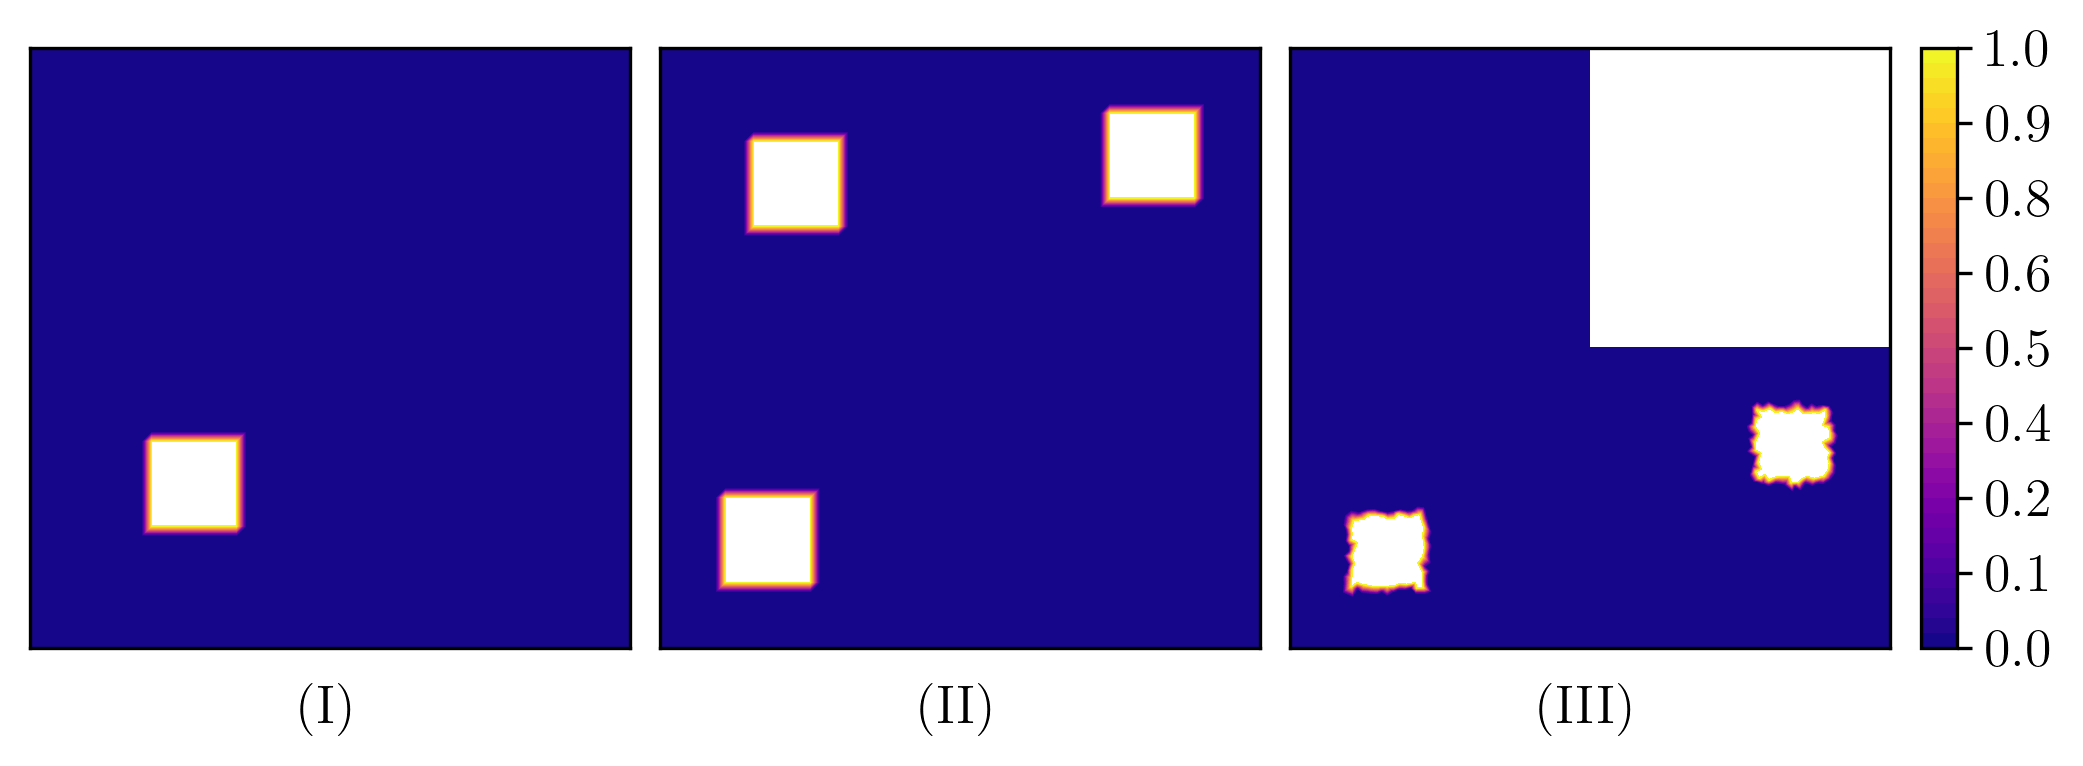
\includegraphics[width=1.0\textwidth]{problem_illustration.png}}
    \caption{The test problems used for the results: Problem~I (left), Problem~II (middle), and Problem~III (right).}
    \label{fig:problem_illustration}
\end{figure*}

Figure~\ref{fig:problem_illustration} shows the three meshes and source functions used throughout the results. Problem I is a square mesh with a single source, used as a baseline. Problem II uses the same geometry with three sources to assess reconstruction under multiple sources. Problem III replaces the square domain with an ``L''-shaped mesh and two sources, introducing a non-convex geometry. Problems I 
and II use a uniform grid, whereas Problem III uses a non-uniform grid.

For all experiments, we set the diffusion coefficient $\sigma = 1$ and the reaction coefficient $c = 1$ in Equation~\eqref{eq:pde}. The finite element space $V_h$ (Equation~\eqref{eq:fem_space}) uses a basis of continuous piecewise-linear hat functions $\phi_i$ (continuous Galerkin, degree 1).

Unless stated otherwise, we use $N = 64^2 = 4096$ for Problems I and II and $N = 6127$ for Problem III, regularization parameter $\lambda = 10^{-4}$, oversampling $p = 5$, and Gaussian random test vectors $\psi_i$ for the rSVD.


\subsection{Computational setup}
All numerical experiments were performed on a laptop running Fedora Linux 43 with Linux kernel version 6.19. The system was running with an Intel(R) Core(TM) i7-10510U (4 cores, 8 threads) with 16GB of memory.

Python 3.9 was used for all computations, together with NumPy and SciPy for linear algebra routines \cite{harrisArrayProgrammingNumPy2020,virtanenSciPy10Fundamental2020}. The FEniCS software was used for solving PDEs using the finite element method \cite{alnaesFEniCSProjectVersion2015,loggAutomatedSolutionDifferential2012}. All library specifications, algorithm implementations, and notebooks used to generate the results in this paper are openly available at: \href{https://github.com/EliasSev/masters-thesis}{github.com/EliasSev/masters-thesis}.


\subsection{Performance metrics}\label{sec:performance_metrics}
Let $x \in \mathbb{R}^N$ denote the true source (its coefficient vector) and $\hat x \in \mathbb{R}^N$ its corresponding reconstruction. To evaluate reconstruction quality, we consider three performance metrics: Euclidean error, EMD, and AUC-IoU.


\paragraph{Earth mover's distance.} The earth mover's distance measures the dissimilarity between two distributions, which in our case refers to $x$ and $\hat x$. Let $x_d$ and $\hat x_d$ be the normalized distributions of $x$ and $\hat x$, respectively, computed as
\begin{equation*}
    (x_d)_i = \frac{|x_i|}{\sum_{j=1}^N |x_j|}, \quad
    (\hat x_d)_i = \frac{|\hat x_i|}{\sum_{j=1}^N |\hat x_j|}.
\end{equation*}
Let $p_i \in \mathbb{R}^2$ denote the spatial coordinates of the $i$-th node in the mesh. The EMD between $x_d$ and $\hat x_d$ is
\begin{equation*}
    \operatorname{EMD}(x_d, \hat x_d) =
    \inf_{\gamma \in \Pi}
    \sum_{i,j=1}^N \gamma_{ij}\, \| p_i - p_j \|,
\end{equation*}
where $\Pi$ is the set of all joint distributions with marginals $x_d$ and $\hat x_d$ \cite{rubnerMetricDistributionsApplications1998}.


\paragraph{AUC-IoU.} The IoU, known as the Jaccard index in statistics, measures the similarity between two sets. It is defined as the size of intersection divided by the size of the union \cite{raschkaPythonMachineLearning}.

We define the binary mask of $x$ at threshold $\tau \in (0, 1)$ as the set
\begin{equation*}
    S_{\tau}(x) = \{ i : x_i \ge \tau \operatorname{max}(x) \}.
\end{equation*}
Then, the IoU of $x$ and $\hat x$ at threshold $\tau$ is the IoU of their binary masks,
\begin{equation*}
    \operatorname{IoU}(\tau) =
    \frac{|S_\tau(x) \cap S_\tau(\hat x)|}{|S_\tau(x) \cup S_\tau(\hat x)|}.
\end{equation*}
Here, $| \cdot |$ denotes the number of elements of a set (its cardinality).

The AUC-IoU is then the integration of the $\operatorname{IoU}(\tau)$ curve,
\begin{equation*}
    \operatorname{AUC-IoU} = \int_{0}^{1} \operatorname{IoU}(\tau) \, d\tau.
\end{equation*}
This can be approximated using the Trapezoidal rule. The AUC-IoU lies in $[0, 1]$, with 1 being a perfect score.


%%%%%%%%%%%%%%%%%%%%%%%%%%%%%%%%%%%%%%%%%%%%%%%%%%%%%%%%%%%%%
% Matrix-free Randomized SVD Part 
%%%%%%%%%%%%%%%%%%%%%%%%%%%%%%%%%%%%%%%%%%%%%%%%%%%%%%%%%%%%%
\subsection{Matrix-free rSVD}
\subsubsection{Computational time}\label{sec:computational_time}
\begin{figure*}[thbp]
    \centerline{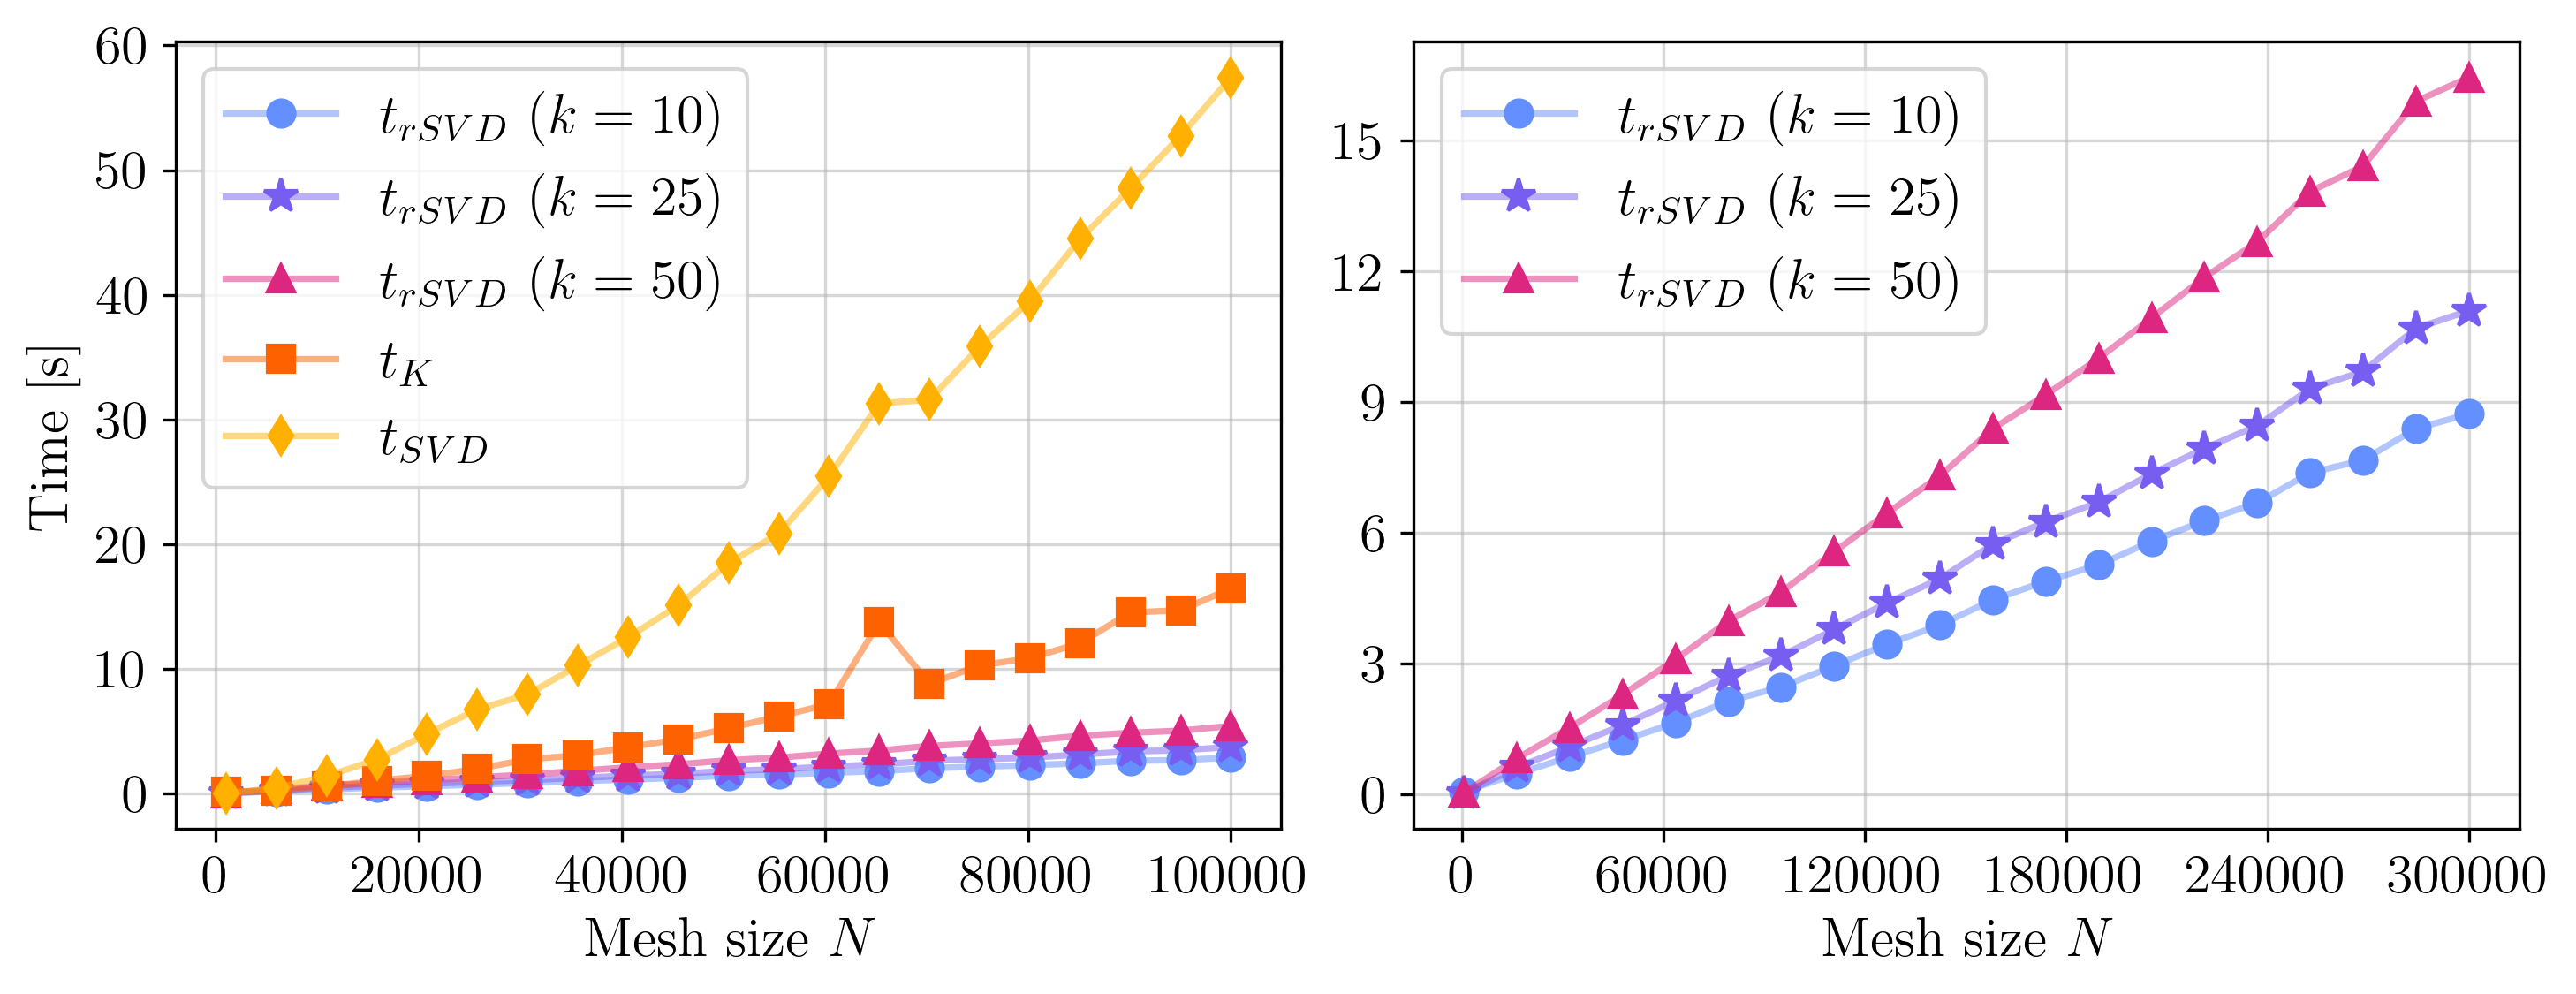
\includegraphics[width=1.0\textwidth]{rsvd_computational_time_comp.png}}
    \caption{Computational time of using Algorithm~\ref{alg:discrete_rsvd} ($t_{\text{rSVD}}$), explicitly forming $K$ ($t_K$), and computing the SVD of $K$ ($t_{\text{SVD}}$) for increasing $N$. Forming $K$ and computing its SVD are infeasible for large $N$, so $t_K$ and $t_{\text{SVD}}$ are omitted from the right plot. Median values over 30 runs, measured in seconds.}
    \label{fig:rsvd_computational_time_comp}
\end{figure*}
\begin{table}[ht]
\centering
    \begin{tabular}{c c c c c c}
    \toprule
        $N$ &
        $\tfrac{t^{(25)}_{\text{rSVD}}}{t^{(10)}_{\text{rSVD}}}$ &
        $\tfrac{t^{(50)}_{\text{rSVD}}}{t^{(10)}_{\text{rSVD}}}$ & 
        $\tfrac{t_K + t_{\text{SVD}}}  {t^{(10)}_{\text{rSVD}}}$ &
        $\tfrac{t_K + t_{\text{SVD}}}  {t^{(25)}_{\text{rSVD}}}$ &
        $\tfrac{t_K + t_{\text{SVD}}}  {t^{(50)}_{\text{rSVD}}}$ \\
    \midrule
        1,000   & 0.79 & 1.14 & 4.21  & 5.31  & 3.68 \\
        25,750  & 1.29 & 1.77 & 11.81 & 9.13  & 6.68 \\
        50,500  & 1.26 & 1.85 & 16.21 & 12.84 & 8.78 \\
        75,250  & 1.27 & 1.85 & 21.13 & 16.61 & 11.39 \\
        100,000 & 1.29 & 1.87 & 25.47 & 19.76 & 13.62 \\
    \bottomrule
    \end{tabular}

\caption{Computational time ratios: $t^{(k)}_{\text{rSVD}}$ at $k = 25$ and $k = 50$ relative to $k = 10$, and $(t_K + t_{\text{SVD}})$ relative to $t^{(k)}_{\text{rSVD}}$ for $k = 10, 25, 50$. Medians over 30 runs.
} 
\label{tab:rsvd_computational_time_comp}
\end{table}
The left plot of Figure~\ref{fig:rsvd_computational_time_comp} shows the computational time of Algorithm~\ref{alg:discrete_rsvd} for target ranks $k = 10,\, 25$ and $50$, compared to forming $K = T A_h^{-1} M$ explicitly (Section~\ref{sec:rsvd}) and taking its SVD. Table~\ref{tab:rsvd_computational_time_comp} shows the relative speedup comparing different methods, with notation $t^{(k)}_{\text{rSVD}}$ for the time of using Algorithm~\ref{alg:discrete_rsvd} at target rank $k$.

The time $t_K$ surpasses $t_{\text{rSVD}}$ for $N > 1000$ across the selected target ranks, and $t_{\text{SVD}}$ surpasses $t_{\text{rSVD}}$ for $N > 5000$. The time $t_{K}$ increases more rapidly than $t_{\text{rSVD}}$ for all target ranks, and $t_{\text{SVD}}$ is observed to increase faster than $t_{K}$, matching their respective theoretical costs of $\mathcal{O}(N_b^2 N)$ and $\mathcal{O}(N_b N \log N)$, established in Section~\ref{sec:rsvd}.
 
The computational times $t_{\text{rSVD}}$ for target ranks $10$, $25$ and $50$ are seen to scale near linearly on this range of $N$ (right plot of Figure~\ref{fig:rsvd_computational_time_comp}). The rate of increase depends on the target rank, with a higher target rank resulting in a more rapid increase. For $N>10{,}000$, increasing $k$ from 10 to 50 results in an increase of $t_{\text{rSVD}}$ by a factor of approximately 1.9, and increasing $k$ from 10 to 25 has a factor of approximately 1.3. 


\subsubsection{Computational breakdown}\label{sec:computational_breakdown}
\begin{figure*}[thbp]
    \centerline{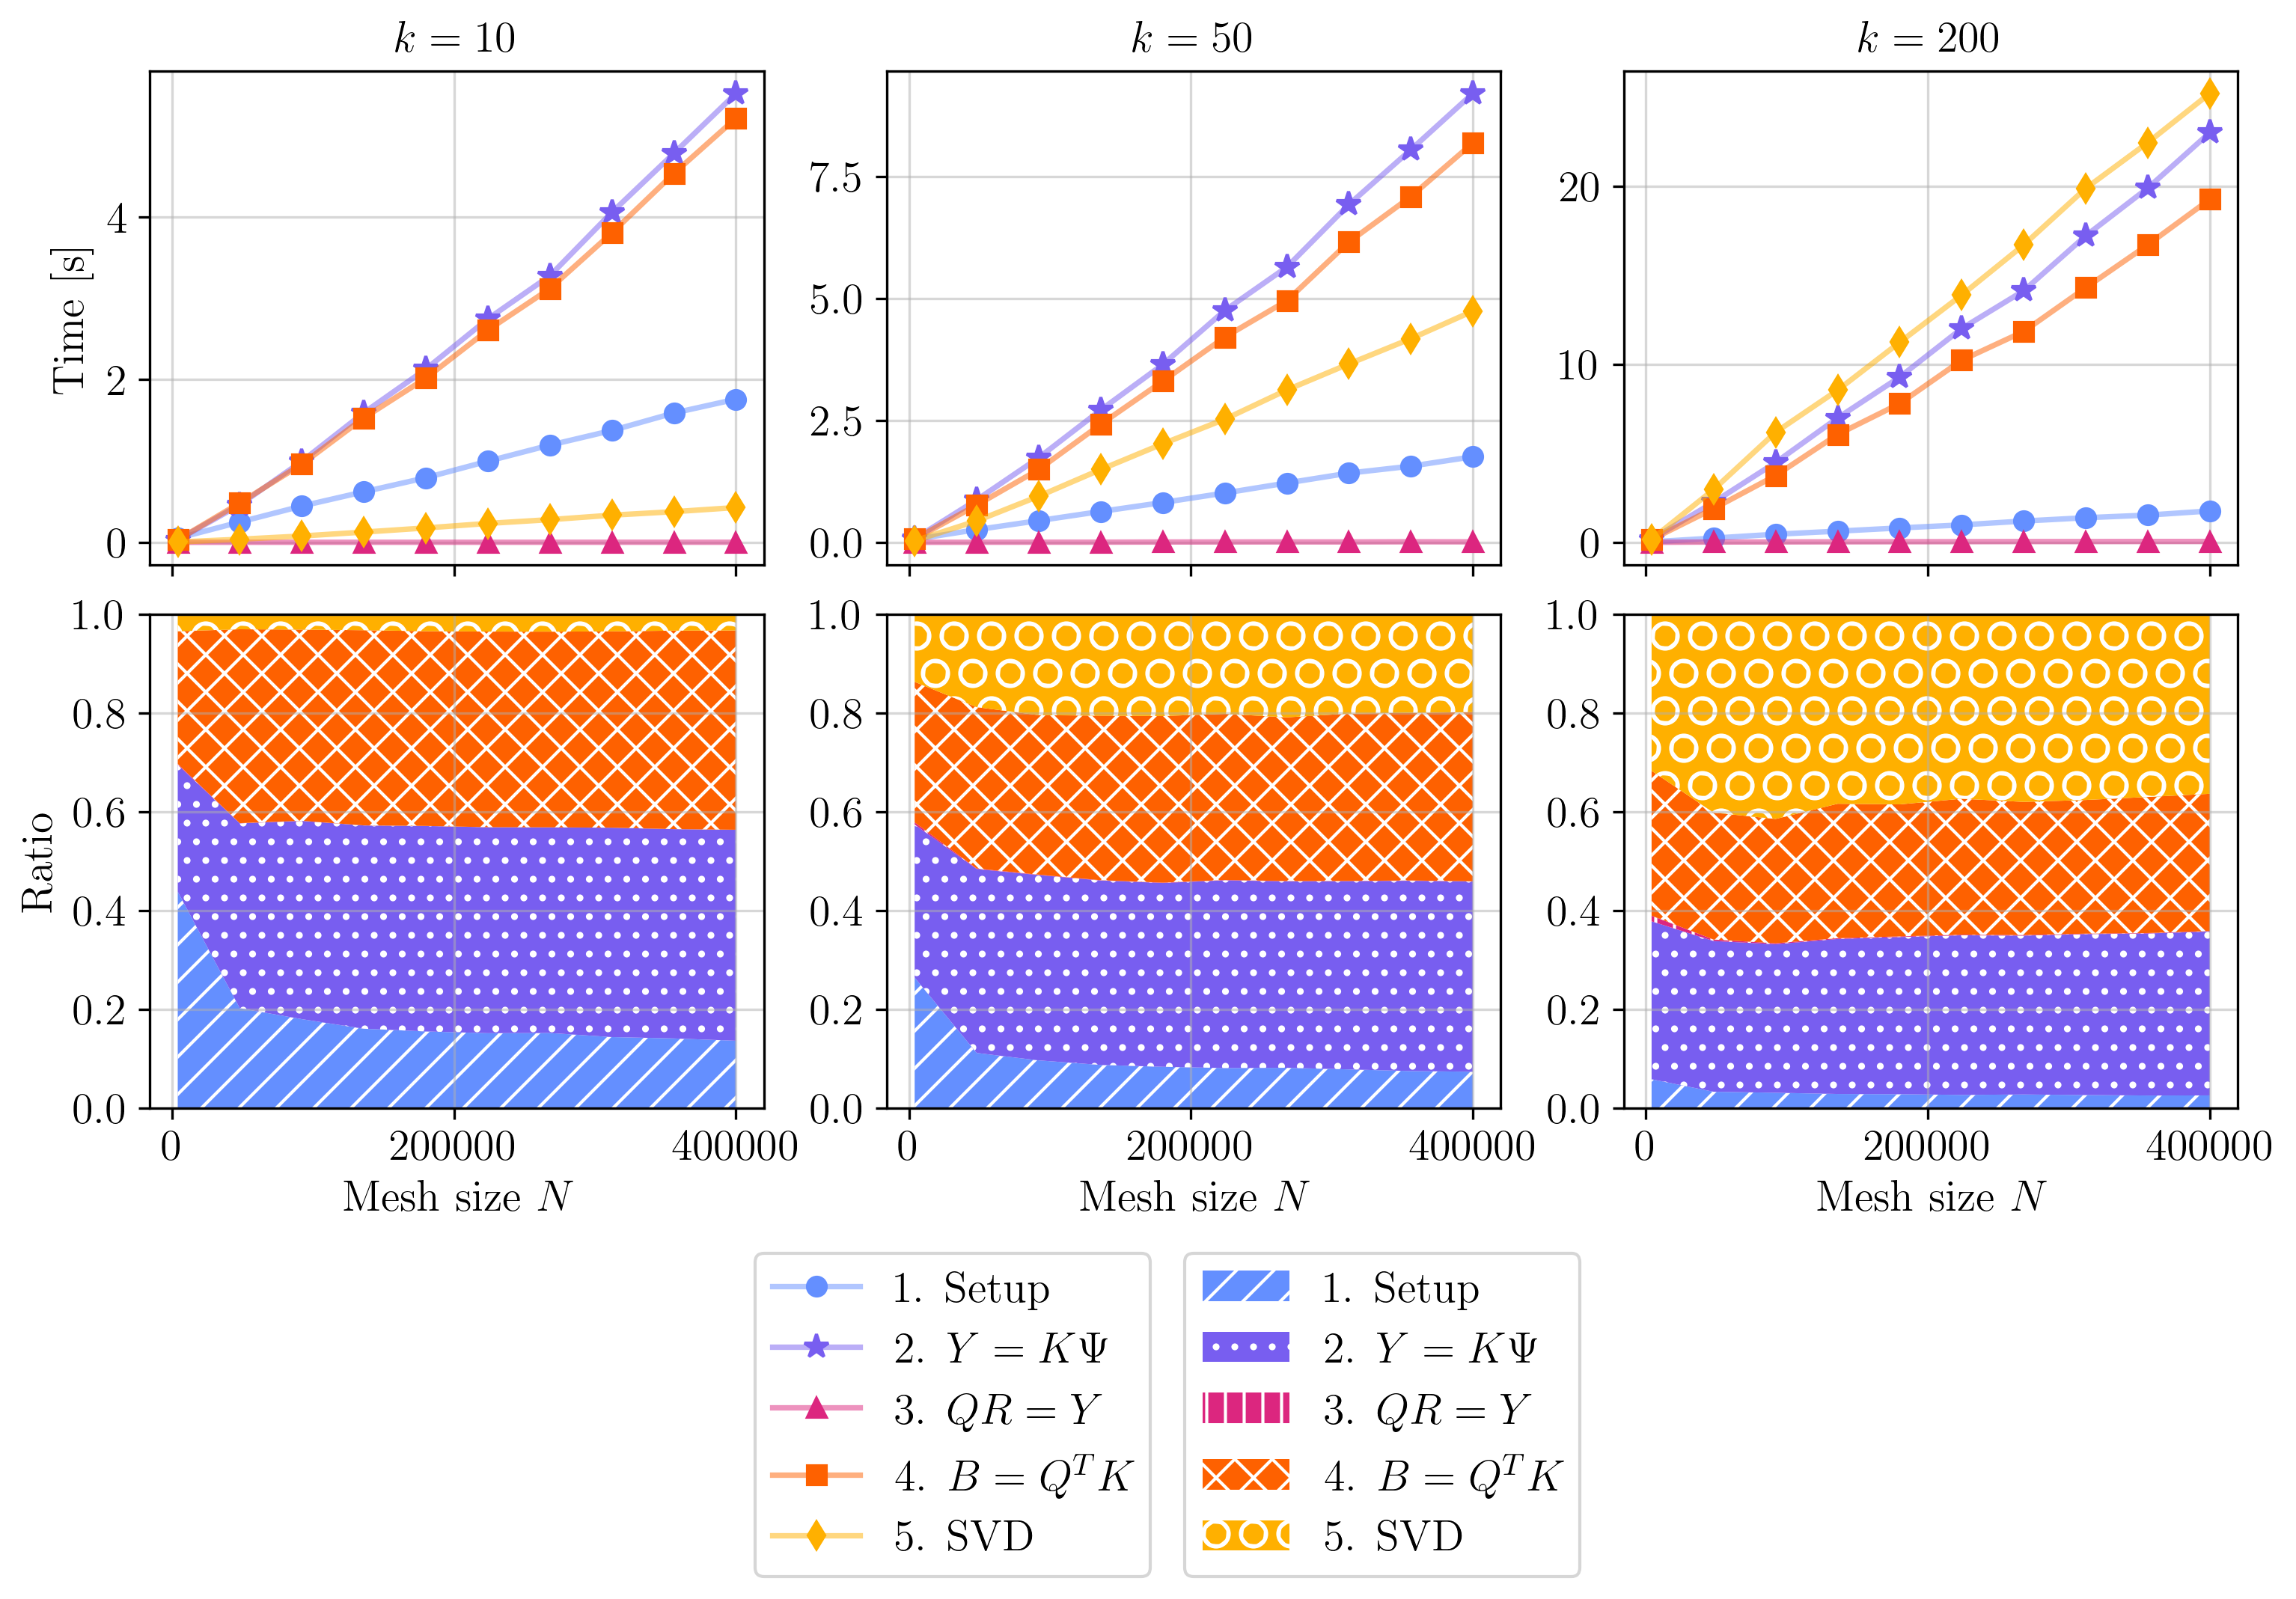
\includegraphics[width=1.0\textwidth]{rsvd_computational_breakdown.png}}
    \caption{Median computational time per stage in Algorithm~\ref{alg:discrete_rsvd} for selected $N$ and increasing $k$. Bottom row shows relative cost. The median is taken over 30 runs for $N \le 40{,}000$ and 10 runs for $N = 400{,}000$}
    \label{fig:rsvd_computational_breakdown}
\end{figure*}
\begin{table}[ht]
\centering
    \begin{tabular}{cc ccccc}
    \toprule
    $N$ & $k$ & Setup & $Y=K\Psi$ & $QR=Y$ & $B=Q^T K$ & SVD \\
    \midrule
    \multirow{3}{*}{$4{,}000$}
    & 10  & 0.44 & 0.26 & 0.00 & 0.27 & 0.03 \\
    & 50  & 0.26 & 0.31 & 0.00 & 0.28 & 0.14 \\
    & 200 & 0.06 & 0.32 & 0.01 & 0.29 & 0.32 \\
    
    \midrule
    \multirow{3}{*}{$180{,}000$}
    & 10  & 0.16 & 0.42 & 0.00 & 0.39 & 0.03 \\
    & 50  & 0.08 & 0.37 & 0.00 & 0.34 & 0.21 \\
    & 200 & 0.03 & 0.32 & 0.00 & 0.27 & 0.39 \\

    \midrule
    \multirow{3}{*}{$400{,}000$}
    & 10  & 0.14 & 0.43 & 0.00 & 0.40 & 0.03 \\
    & 50  & 0.07 & 0.39 & 0.00 & 0.34 & 0.20 \\
    & 200 & 0.03 & 0.33 & 0.00 & 0.28 & 0.36 \\
    \bottomrule
    \end{tabular}
\caption{Relative computational cost of each stage in Algorithm~\ref{alg:discrete_rsvd} for selected target ranks $k$ and mesh sizes $N$.}
\label{tab:rsvd_computational_breakdown}
\end{table}
Figure~\ref{fig:rsvd_computational_breakdown} shows the median computational time for each stage of Algorithm~\ref{alg:discrete_rsvd} for selected $N$ and increasing $k$, with the relative computational cost shown in the bottom row. The `Setup' stage includes factorization of the mass matrix $M_\partial$, and the setup of the $K$ and $K^*$ solvers (Section~\ref{sec:initial_matrix_factorizations}). The remaining stages of Algorithm~\ref{alg:discrete_rsvd} are `2. $Y = K\Psi$' (lines 1--6), `3. $QR = Y$' (lines 7--8), `4. $B = Q^T K$' (lines 9--14), and `5. SVD' (lines 15--18). Table~\ref{tab:rsvd_computational_breakdown} shows relative computational time for selected target ranks and mesh sizes.

The dominant costs of Algorithm~\ref{alg:discrete_rsvd} are the forward solves using $K$ (stage 2) and the adjoint solves using $K^*$ (stage 4), both of which scale roughly linearly with $N$, matching the theoretical cost of $\mathcal{O}(l N \log N)$ with $l = k + p$ (Section~\ref{sec:initial_matrix_factorizations}). The setup stage has theoretical cost $\mathcal{O}(N^{3/2})$ but appears near-linear in $N$ over the range considered here. Its share of total time decreases with $k$, because setup is independent of the target rank.

Stage 5's relative cost is primarily determined by the target rank $k$, but also scales linearly with $N$, matching the predicted $\mathcal{O}(l^2 N)$ cost of the SVD of $B$. Its share grows with $k$: at $N = 400{,}000$, stage 5 accounts for 3\% of total time at $k = 10$ and 36\% at $k = 200$. Stage 3 (the QR factorization of the $N_b \times l$ matrix $Y$) remains below 1\% of total time across all mesh sizes.


\subsubsection{Target rank effect on reconstruction quality}\label{sec:target_rank_reconstruction}
\begin{figure*}[htbp]
\centering

\begin{subfigure}{1.0\textwidth}
    \centering
    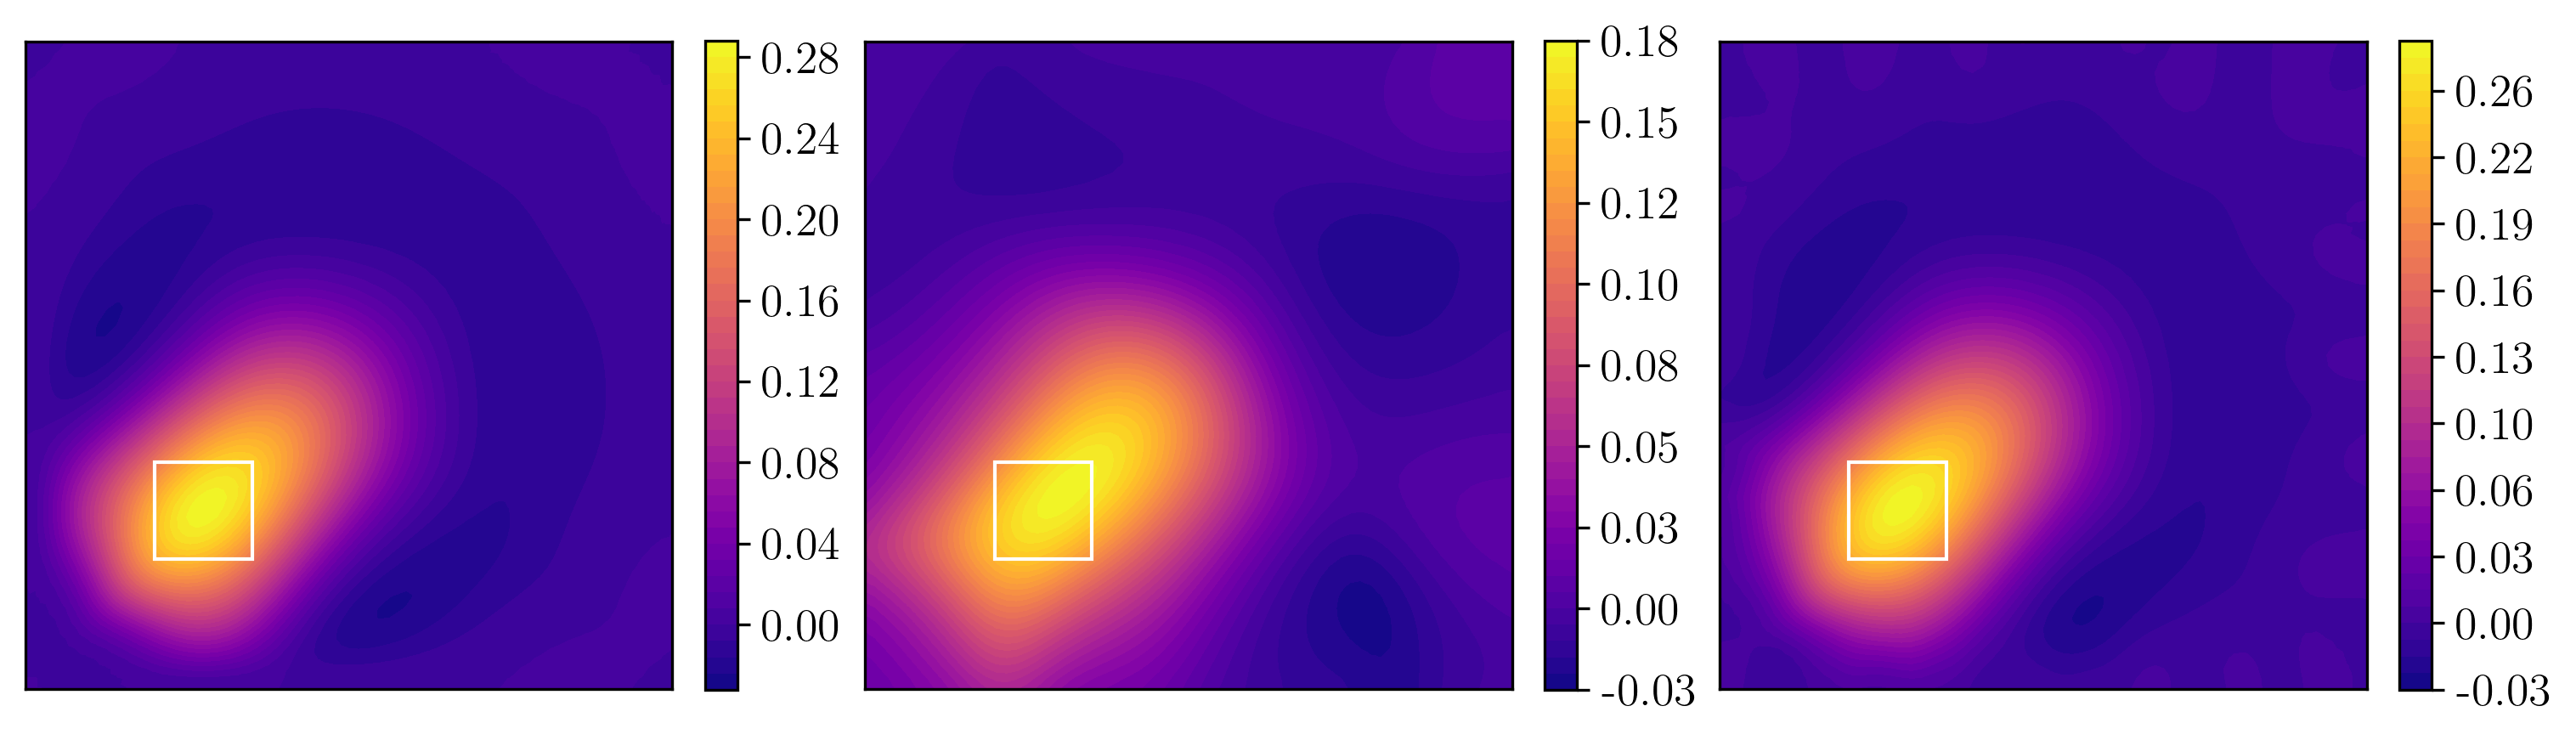
\includegraphics[width=\linewidth]{test_problem_I.png}
    \caption{Problem I.}
    \label{fig:test_problem_I}
\end{subfigure}

\vspace{0.5cm}

\begin{subfigure}{1.0\textwidth}
    \centering
    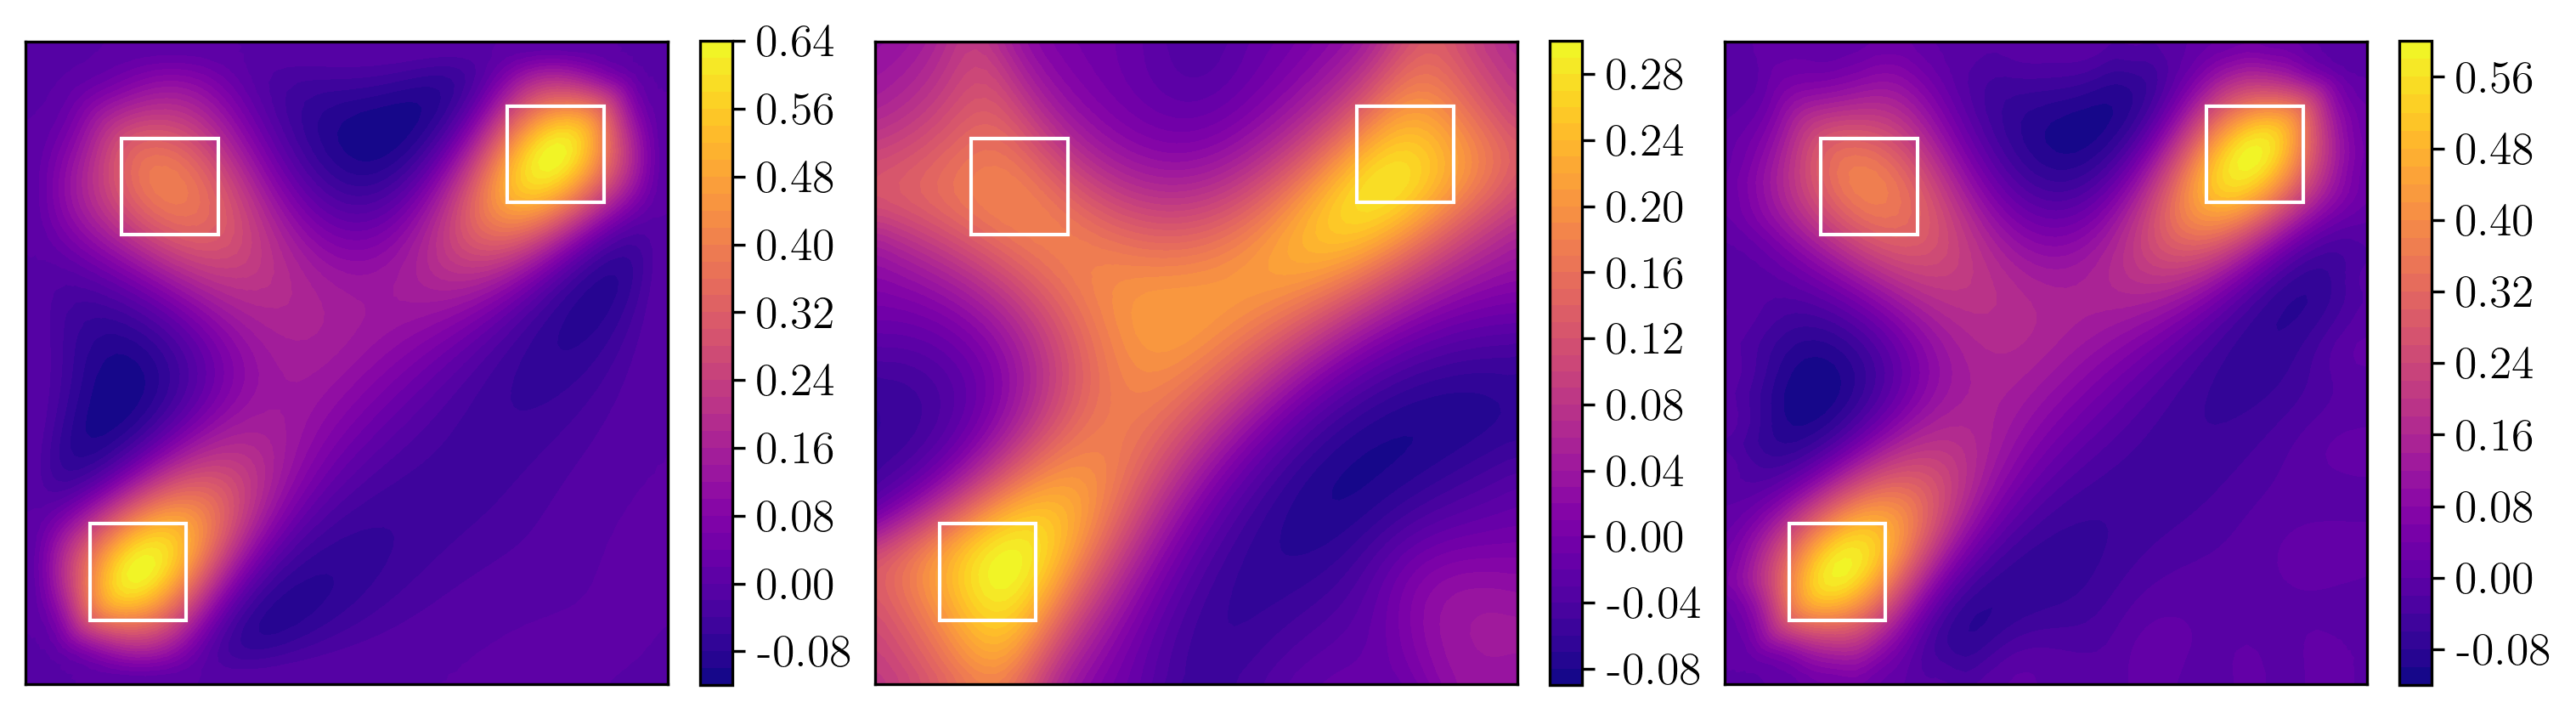
\includegraphics[width=\linewidth]{test_problem_II.png}
    \caption{Problem II.}
    \label{fig:test_problem_II}
\end{subfigure}

\vspace{0.5cm}

\begin{subfigure}{1.0\textwidth}
    \centering
    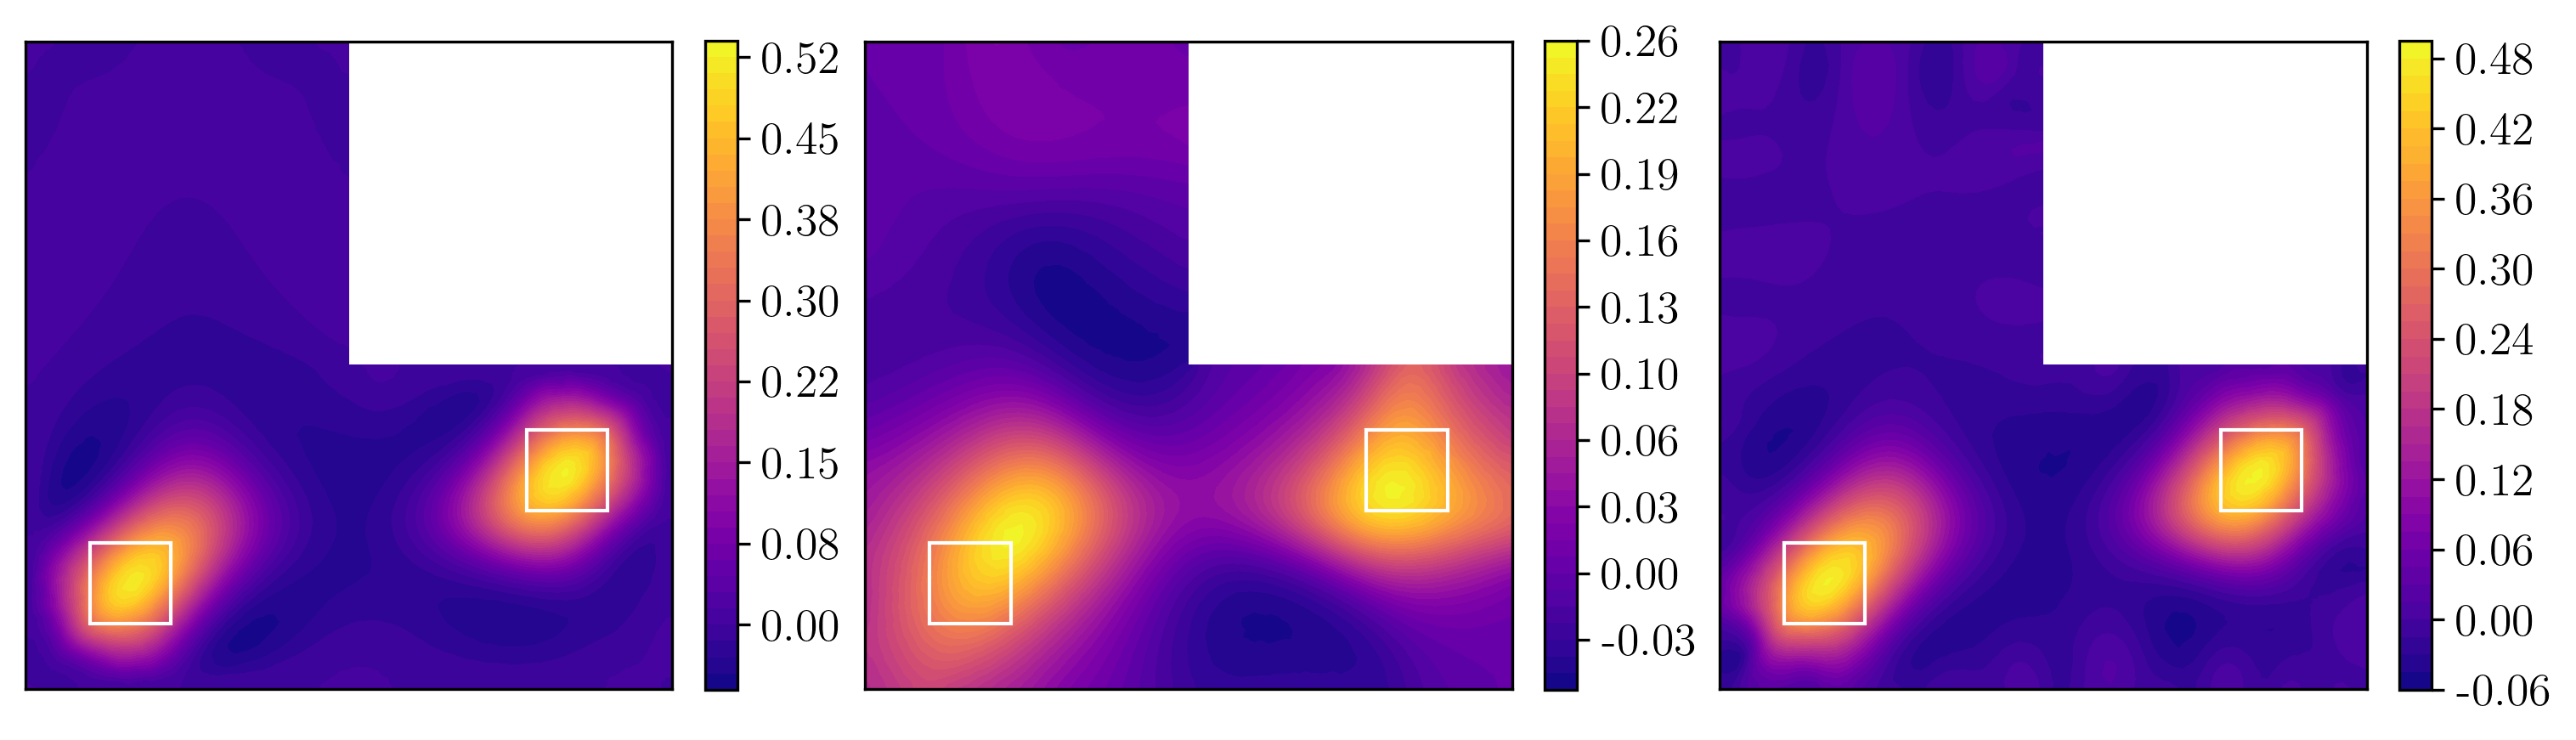
\includegraphics[width=\linewidth]{test_problem_III.png}
    \caption{Problem III.}
    \label{fig:test_problem_III}
\end{subfigure}

\caption{Weighted Tikhonov solutions using exact $K$ and $W$ (left), a rank-$10$ rSVD approximation of $K$ and $W$ (middle), and a rank-$50$ rSVD approximation (right), for Problems~I, II, and III. True source location outlined in white (Figure~\ref{fig:problem_illustration}).}
\label{fig:test_problems_selected}
\end{figure*}

Figure~\ref{fig:test_problems_selected} shows the weighted Tikhonov solution of Equation~\eqref{eq:discrete_inverse_problem}, with $K$ and $W$ either exact or approximated by Algorithm~\ref{alg:discrete_rsvd} at target ranks $k = 10$ and $k = 50$.

For Problem~I (Figure~\ref{fig:test_problem_I}) at $k = 10$, the location of the source is partially identified (middle), slightly shifted towards the interior and with more smoothing than the exact Tikhonov solution (left). The weighted Tikhonov regularization itself already produces significant smoothing \cite{elvetunRegularizationOperatorSource2020}, and low-rank approximations amplify this effect at small $k$. At $k = 50$ (right), the reconstruction is visually identical to the exact Tikhonov solution. In Problems~II and~III (Figures~\ref{fig:test_problem_II} and~\ref{fig:test_problem_III}), $k = 10$ shows the same over-smoothing and shift of each source. These issues disappear at $k = 50$. Across all three problems, $k = 50$ matches the exact Tikhonov reconstruction visually at a small fraction of the computational cost of solving the exact problem (Section~\ref{sec:computational_time}).

\begin{figure*}[htbp]
\centering

\begin{subfigure}{1.0\textwidth}
    \centering
    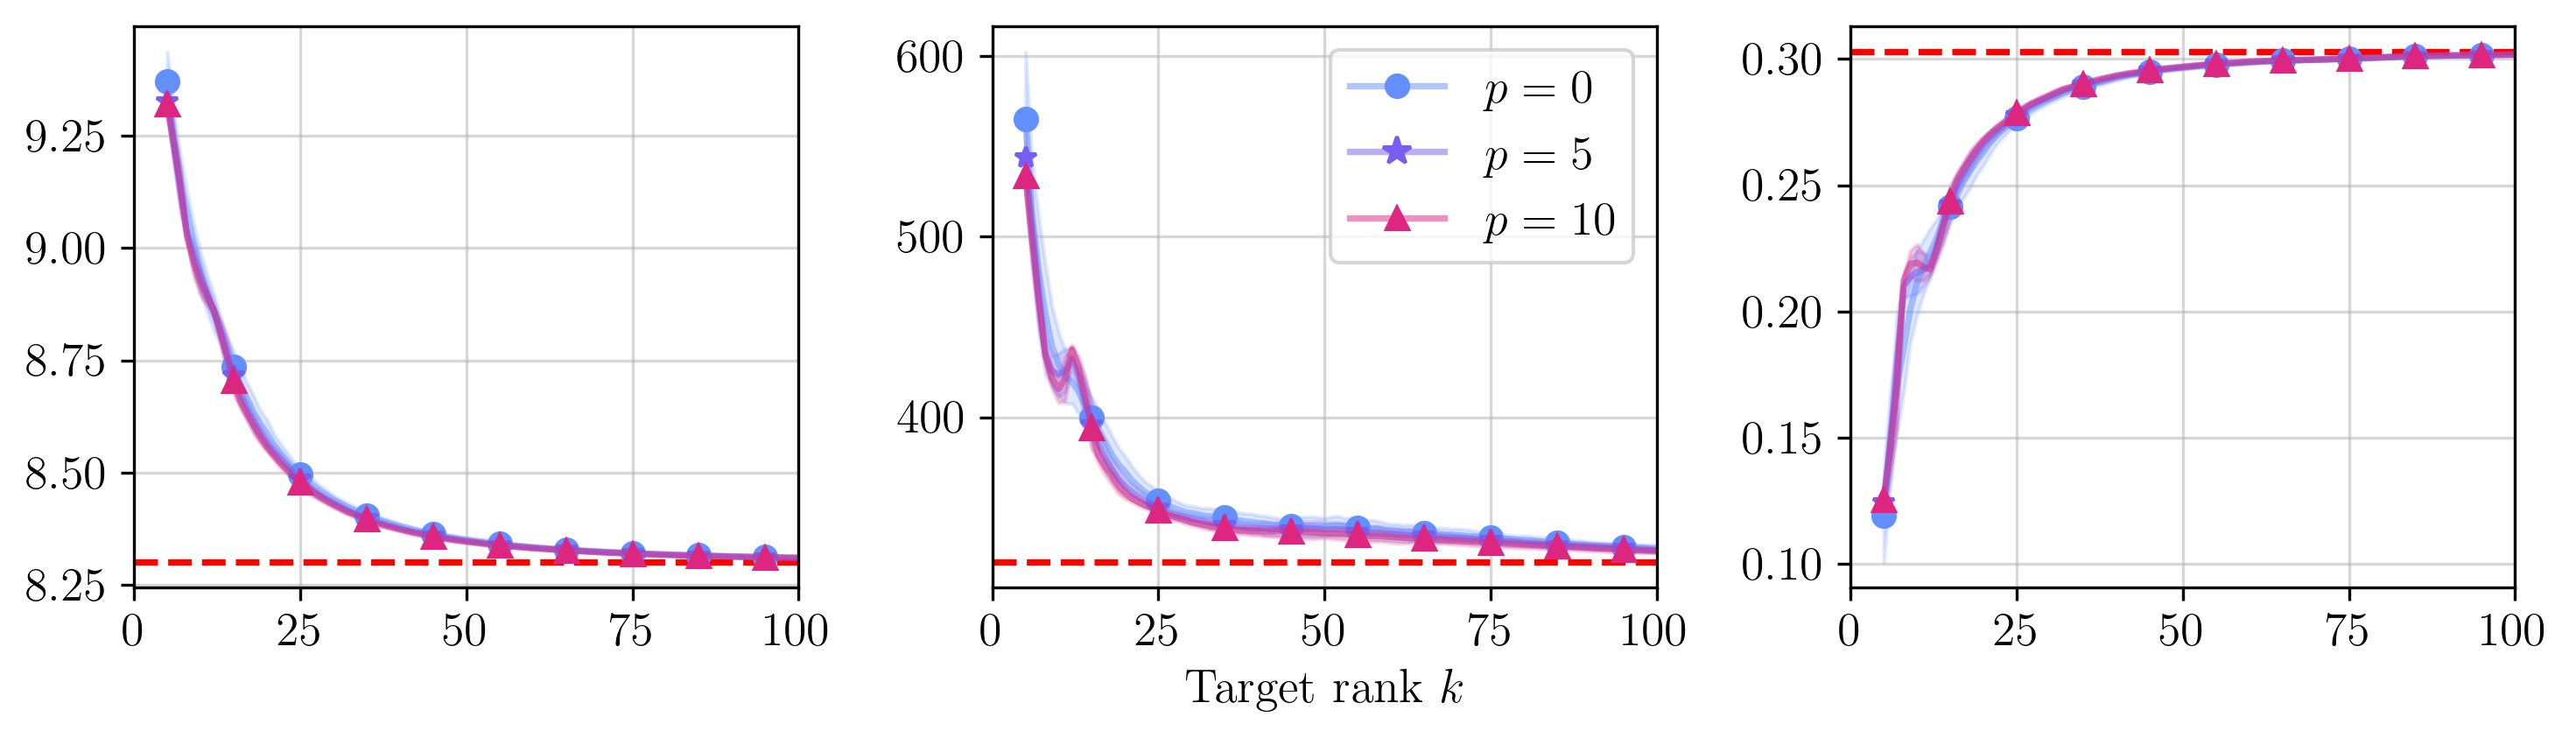
\includegraphics[width=\linewidth]{rsvd_over_k_I.png}
    \caption{Problem I.}
    \label{fig:rsvd_over_k_I}
\end{subfigure}

\vspace{0.5cm}

\begin{subfigure}{1.0\textwidth}
    \centering
    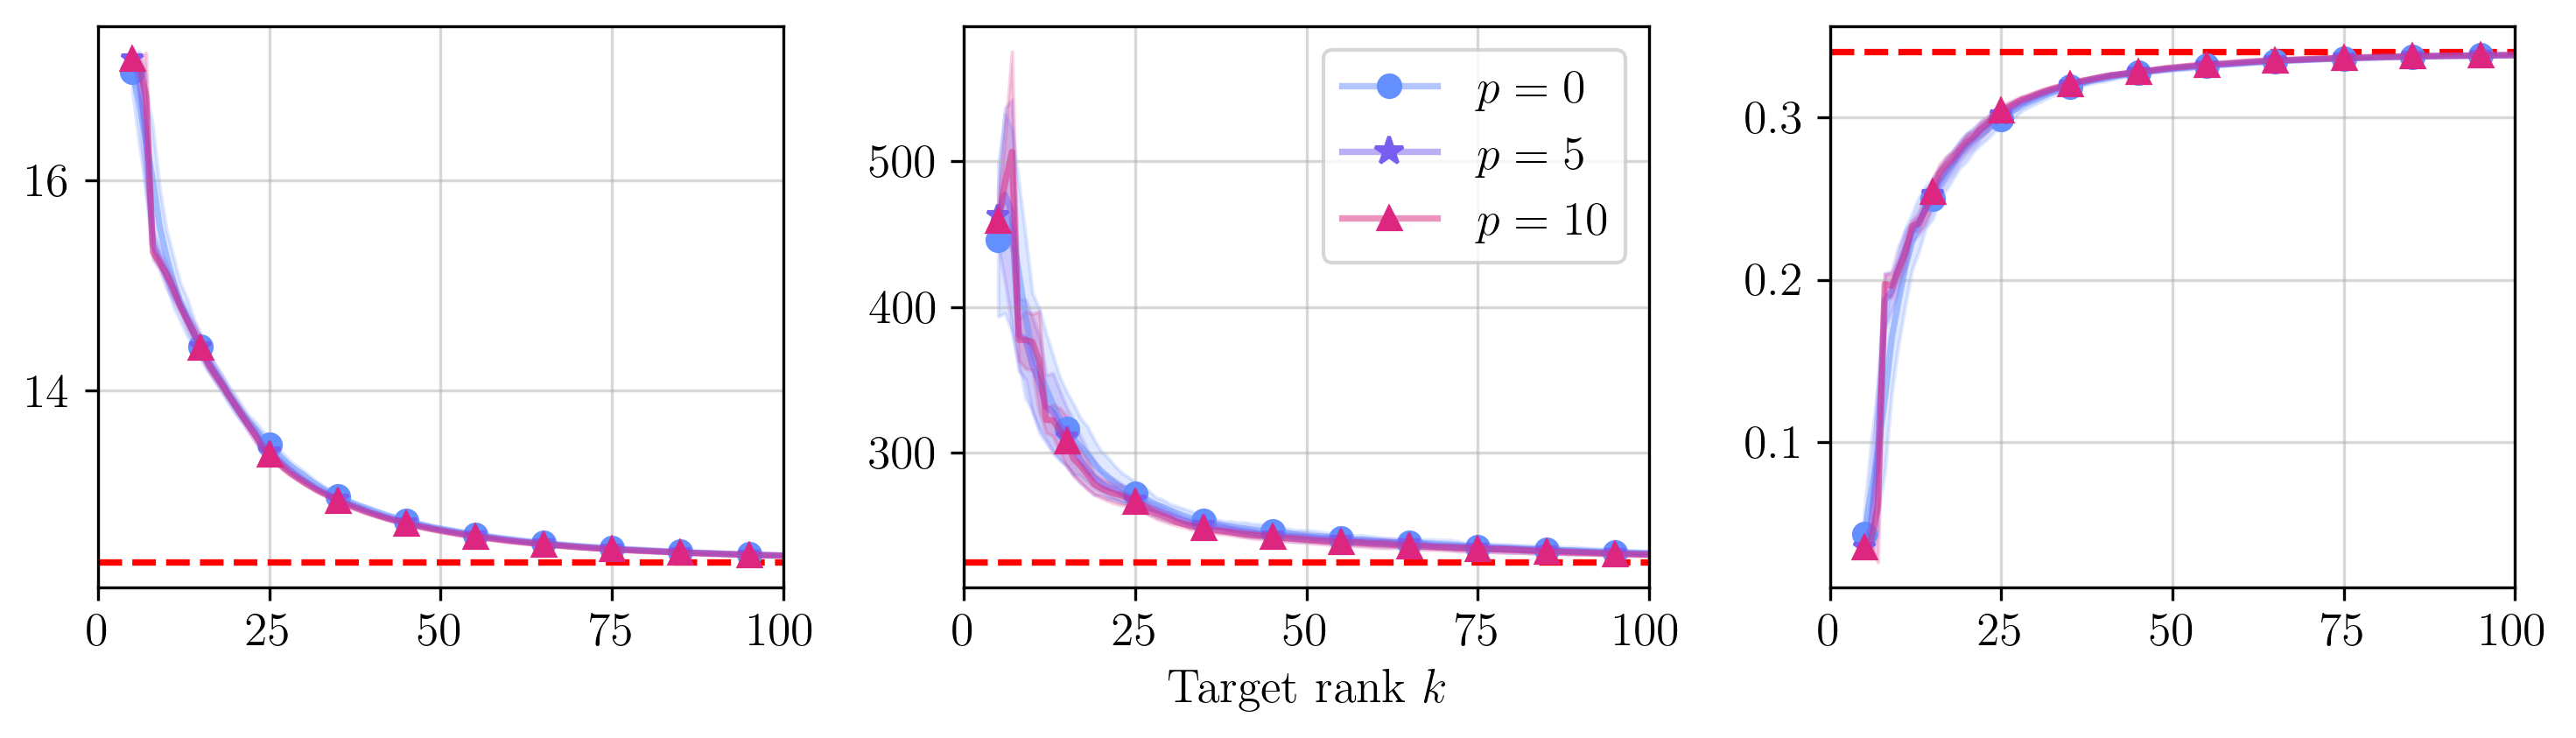
\includegraphics[width=\linewidth]{rsvd_over_k_II.png}
    \caption{Problem II.}
    \label{fig:rsvd_over_k_II}
\end{subfigure}

\vspace{0.5cm}

\begin{subfigure}{1.0\textwidth}
    \centering
    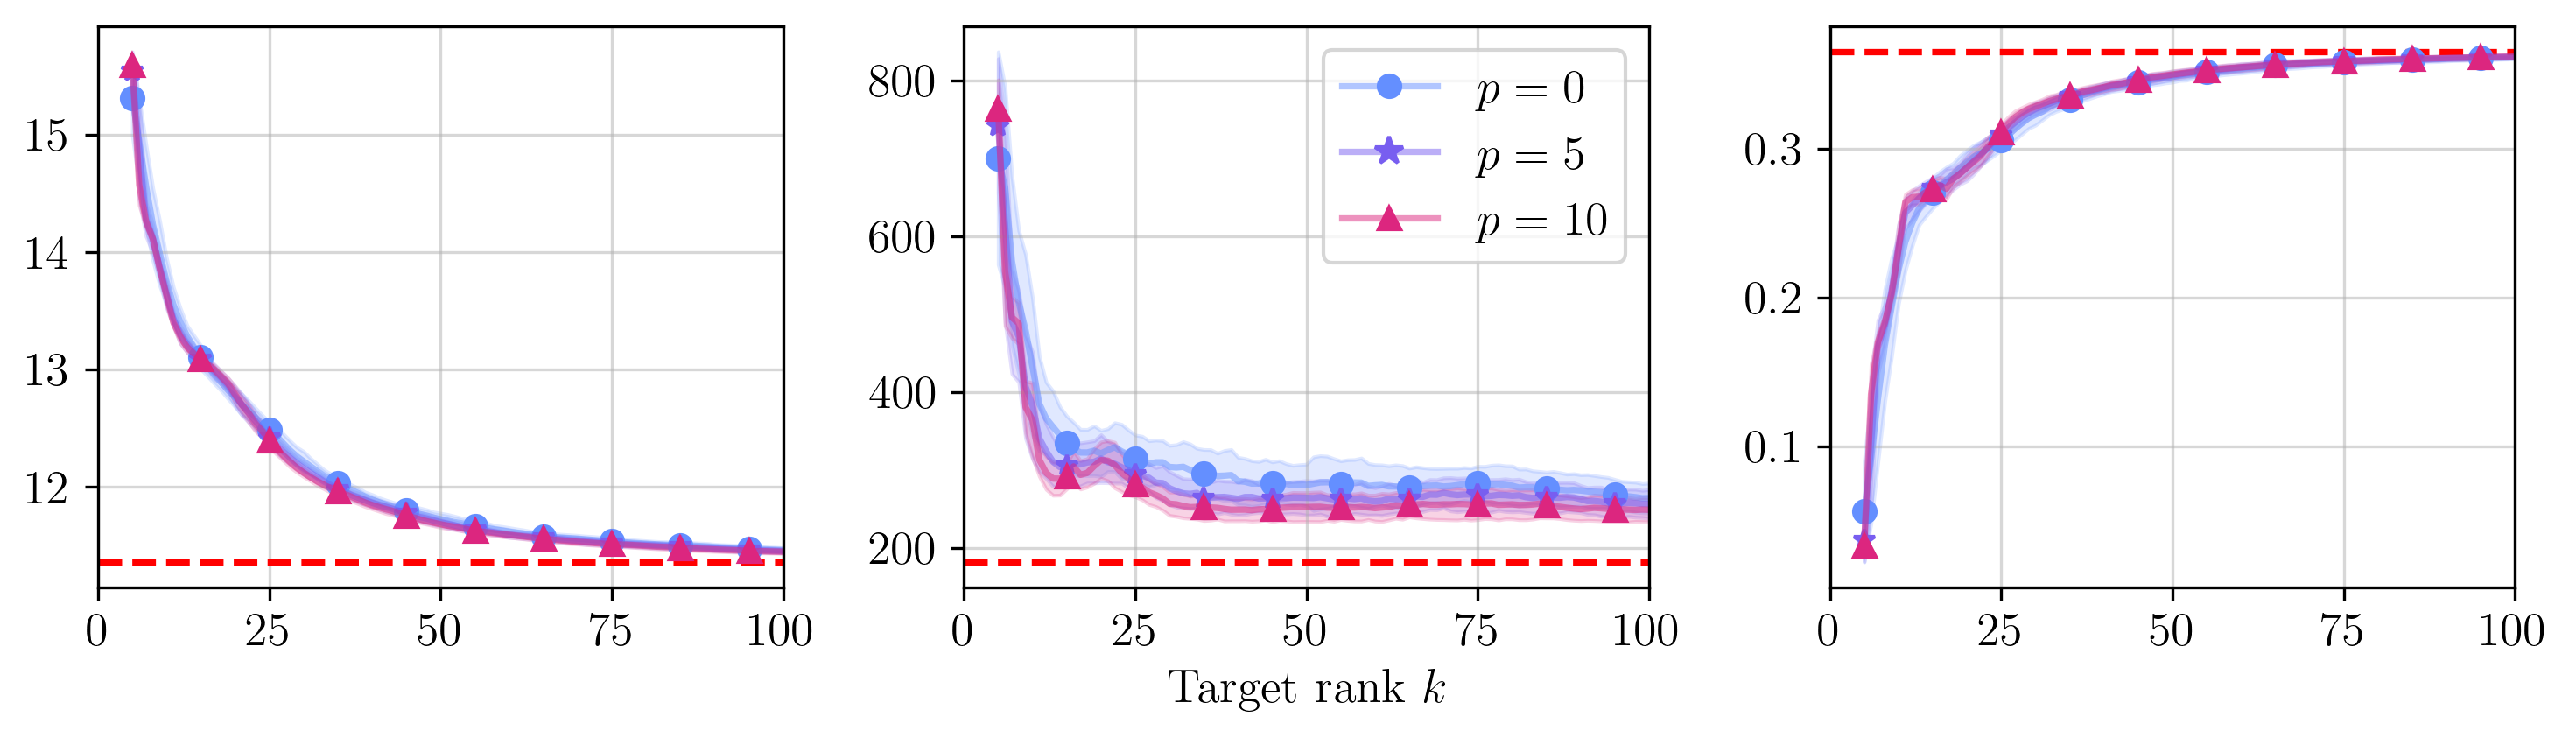
\includegraphics[width=\linewidth]{rsvd_over_k_III.png}
    \caption{Problem III.}
    \label{fig:rsvd_over_k_III}
\end{subfigure}

\caption{Reconstruction error of weighted Tikhonov solutions using rSVD-approximated $K$ and $W$ (solid lines, mean $\pm 1$ standard deviation over 50 runs) versus the exact weighted Tikhonov solution (dashed line), for a range of target ranks $k$ and oversampling parameters $p$. Columns: Euclidean (left), EMD (middle), AUC-IoU (right).}
\label{fig:rsvd_over_k}
\end{figure*}
\begin{table}[ht]
\centering
\begin{tabular}{c ccc ccc ccc}
  \toprule
      & \multicolumn{3}{c}{Euclidean (\%)}
      & \multicolumn{3}{c}{EMD (\%)}
      & \multicolumn{3}{c}{AUC-IoU (\%)} \\
  \cmidrule(lr){2-4}\cmidrule(lr){5-7}\cmidrule(lr){8-10}
  $k$ & I & II & III & I & II & III & I & II & III \\
  \midrule
  10  & 7.49 & 22.40 & 20.49 & 32.00 & 66.57 & 109.80 & 27.91 & 40.53 & 38.26 \\
  25  & 2.18 & 8.44 & 9.34 & 9.11 & 18.68 & 58.86 & 8.06 & 10.85 & 15.40 \\
  50  & 0.56 & 2.44 & 2.92 & 4.74 & 6.44 & 39.13 & 1.97 & 2.87 & 4.07 \\
  100 & 0.11 & 0.50 & 0.78 & 1.79 & 2.03 & 33.66 & 0.38 & 0.59 & 0.88 \\
  199 & 0.01 & 0.05 & 0.15 & 0.12 & 0.16 & 7.85 & 0.01 & 0.02 & 0.04 \\
  \bottomrule
\end{tabular}

\caption{Relative difference (\%) between rSVD error and the full-rank exact solution at selected target ranks $k$, for oversampling $p=5$. Positive values indicate the rSVD solution is worse than the reference. Mean over 50 runs.}
\label{tab:rsvd-over-k}
\end{table}

To measure reconstruction error, we consider three different metrics: Euclidean norm, earth mover's distance (EMD), and the area under the intersection over union curve (AUC-IoU). These metrics emphasize the localization and spatial shape of the reconstructed source, rather than just the amplitude. See Section~\ref{sec:performance_metrics} for details on each metric. An AUC-IoU score of 1 indicates a perfect overlap of the reconstruction and the true source.

Figure~\ref{fig:rsvd_over_k} shows the reconstruction error for target ranks $k \in [5,\, 100]$ and oversampling parameters $p = 0,\, 5,\, 10$. The error curves flatten beyond $k \approx 100$, so the figure is cropped there for more detail at smaller $k$. Table~\ref{tab:rsvd-over-k} gives the relative difference (in \%) between the rSVD and exact Tikhonov solutions at selected $k$.

The rSVD reconstruction error approaches the exact reconstruction error as $k$ increases, for all three error metrics. Larger oversampling $p$ yields a small but consistent reduction in error across all three metrics, most visible in the EMD curves. At $k = 50$ and $p = 5$, the Euclidean relative difference is 0.56\%, 2.44\%, and 2.92\% for Problems~I, II, and III; the AUC-IoU gives 1.97\%, 2.87\%, and 4.07\%; and the EMD gives 4.74\%, 6.44\%, and 39.13\%. The EMD is more sensitive to low-amplitude noise in the reconstruction, which increases its relative error even though the noise is difficult to see in Figure~\ref{fig:test_problems_selected}. At $k = 199$ (the largest rank considered), Euclidean and AUC-IoU are within fractions of a percent of the exact Tikhonov values. The EMD ranges from 0.12\% to 7.85\%, which indicates its sensitivity to small noise or small differences in shape or position compared to the exact Tikhonov solution.


\subsubsection{Test vector distribution effect on error}\label{sec:test_vector_distribution_effect_on_error}
\begin{figure*}[htbp]
    \centerline{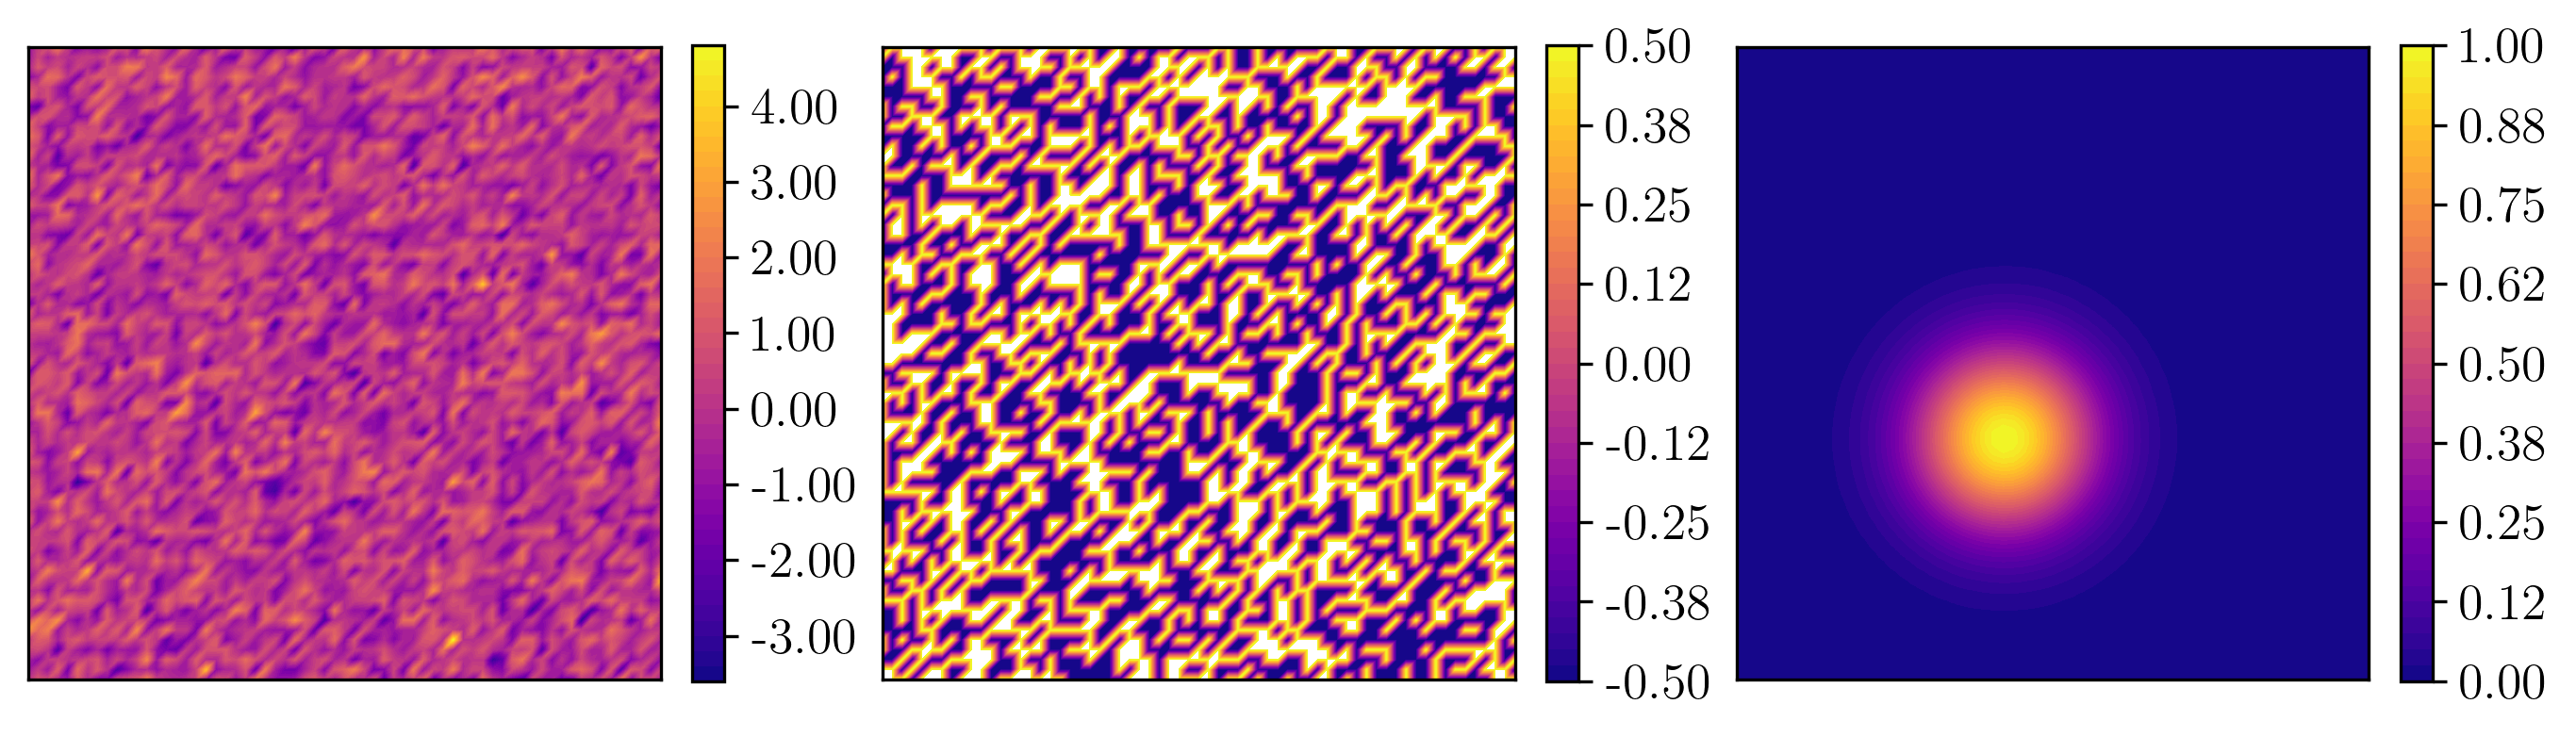
\includegraphics[width=1.0\textwidth]{random_test_vectors.png}}
    \caption{Random test vectors $\psi_i$ drawn from different distributions: Standard Gaussian (left), Rademacher (middle), and Peak (right).}
    \label{fig:random_test_vectors}
\end{figure*}
Three test vector distributions are compared: standard Gaussian ($\psi_{ij} \sim \mathcal{N}(0,1)$), Rademacher ($\psi_{ij} \in \{-\tfrac{1}{2}, \tfrac{1}{2}\}$ with equal probability, see \cite{montgomery-smithDistributionRademacherSums1990}), and a spatially localized Gaussian peak, which we refer to as a Peak test vector:
\begin{equation*}
    \psi_i(x) = \exp\left(-\frac{|x - x_0|^2}{2\sigma_p^2}\right),
\end{equation*}
where the center of the peak $x_0$ is sampled uniformly from the domain and $\sigma_p = 0.1$. Examples are shown in Figure~\ref{fig:random_test_vectors}.

\begin{figure*}[htbp]
    \centerline{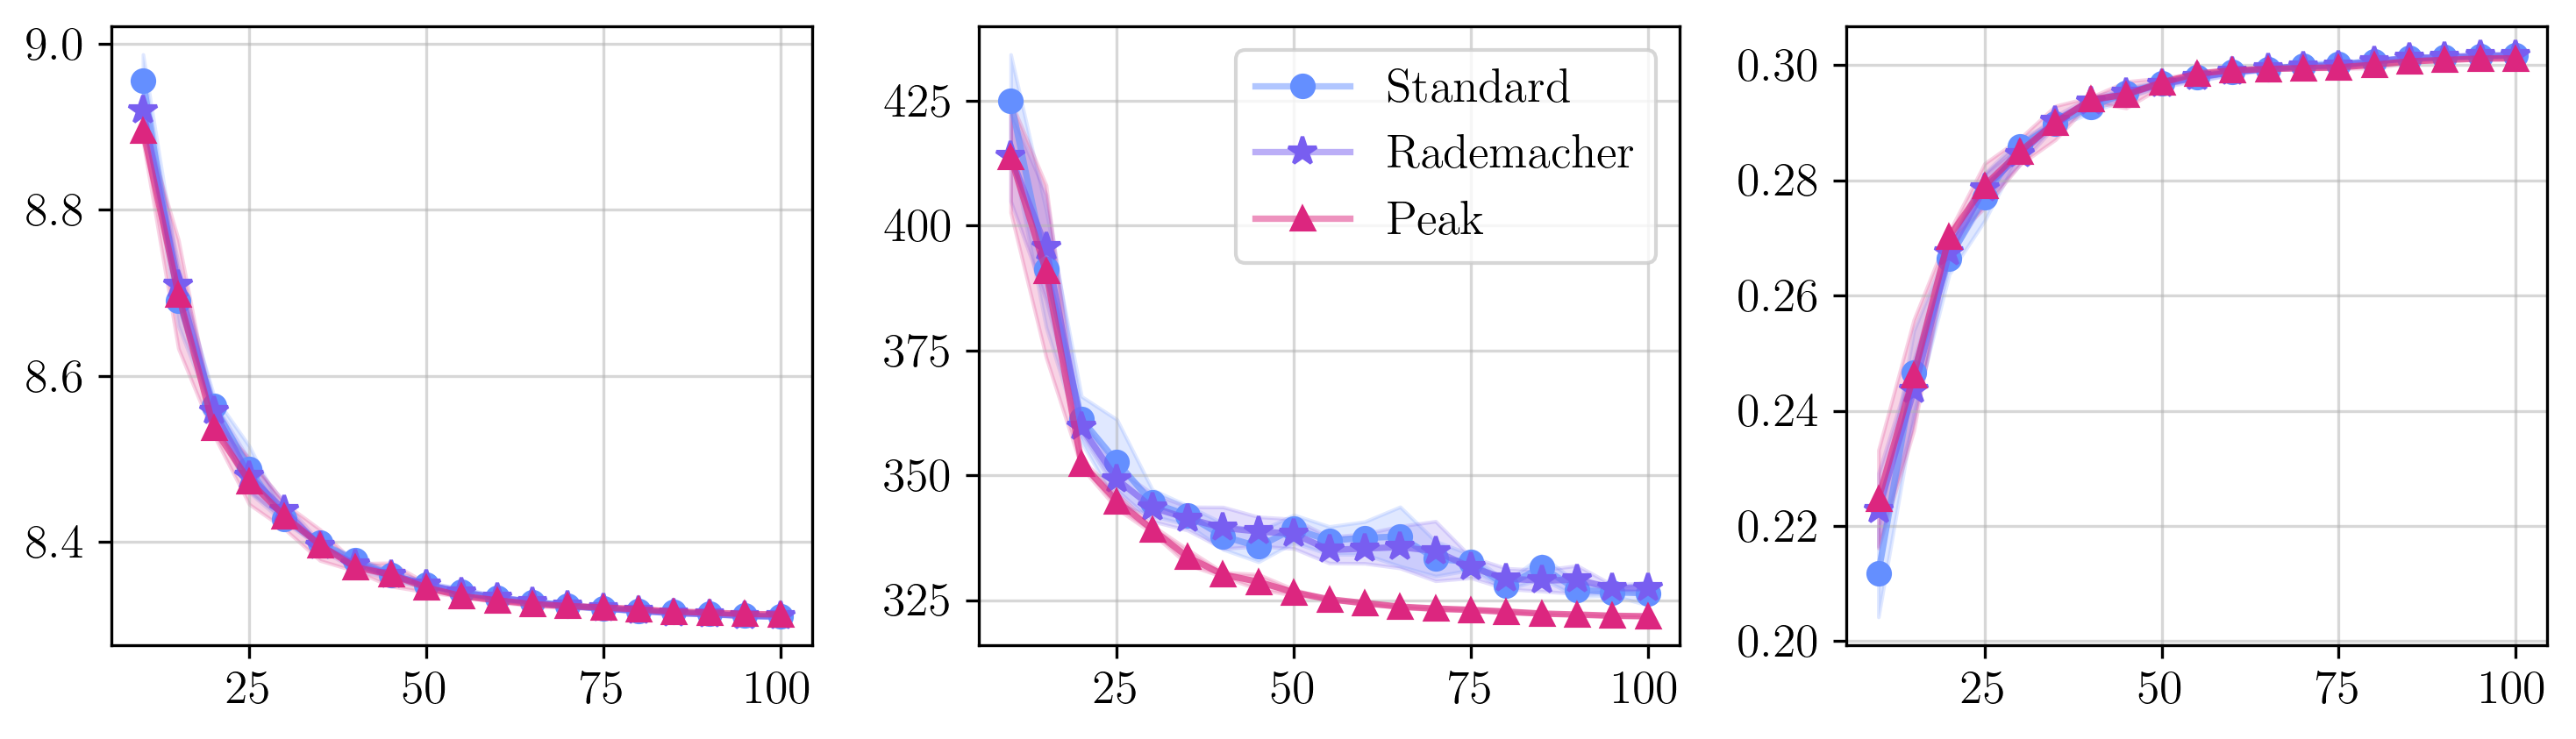
\includegraphics[width=1.0\textwidth]{random_vectors_error.png}}
    \caption{Comparison of reconstruction error using rSVD (Algorithm~\ref{alg:discrete_rsvd}) with sampling vectors $\psi_i$ from different distributions (using Problem I). Error measured in: Euclidean norm (left), EMD (middle), and AUC-IoU (right). Mean $\pm 1$ standard deviation over 50 runs.}
    \label{fig:random_vectors_error}
\end{figure*}
\begin{figure*}[htbp]
    \centerline{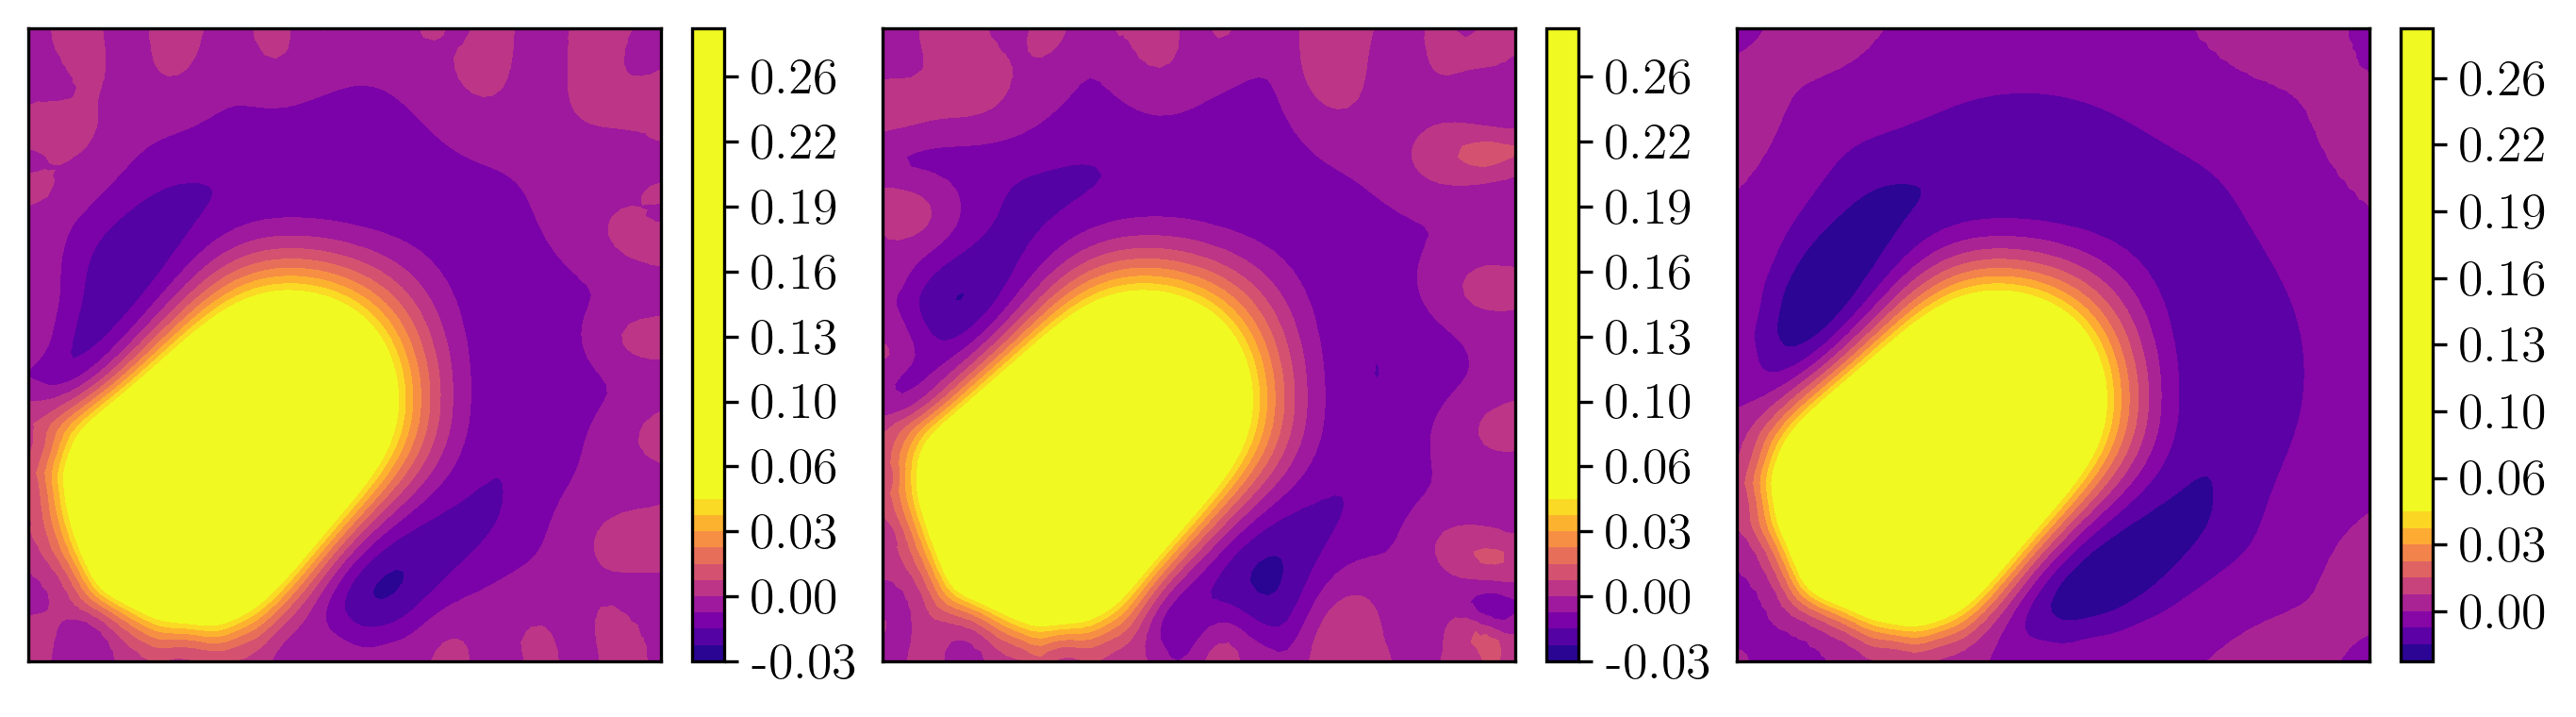
\includegraphics[width=1.0\textwidth]{clipped_random_vectors.png}}
    \caption{Reconstructions using different sampling distributions ($\psi_i$) in the rSVD approximation (Algorithm~\ref{alg:discrete_rsvd}, Problem I, $k = 50$): Standard Gaussian (left), Rademacher (middle), and Peak (right). Colormap clipped to reveal low-amplitude noise.}
    \label{fig:clipped_random_vectors}
\end{figure*}
Figure~\ref{fig:random_vectors_error} compares reconstruction error across the three distributions for Problem~I (similar results hold for Problems~II and III). Rademacher and standard Gaussian test vectors yield nearly identical errors across all three metrics. The Peak test vectors produce lower EMD error and smaller run-to-run variance. Figure~\ref{fig:clipped_random_vectors} shows individual reconstructions with the colormap clipped to $0.05$, revealing that the Peak test vectors generate less low-amplitude noise than Gaussian or Rademacher.


\subsubsection{Mesh resolution effect on reconstruction error}\label{sec:mesh_resolution_effect_on_reconstruction_error}
\begin{figure*}[thbp]
    \centerline{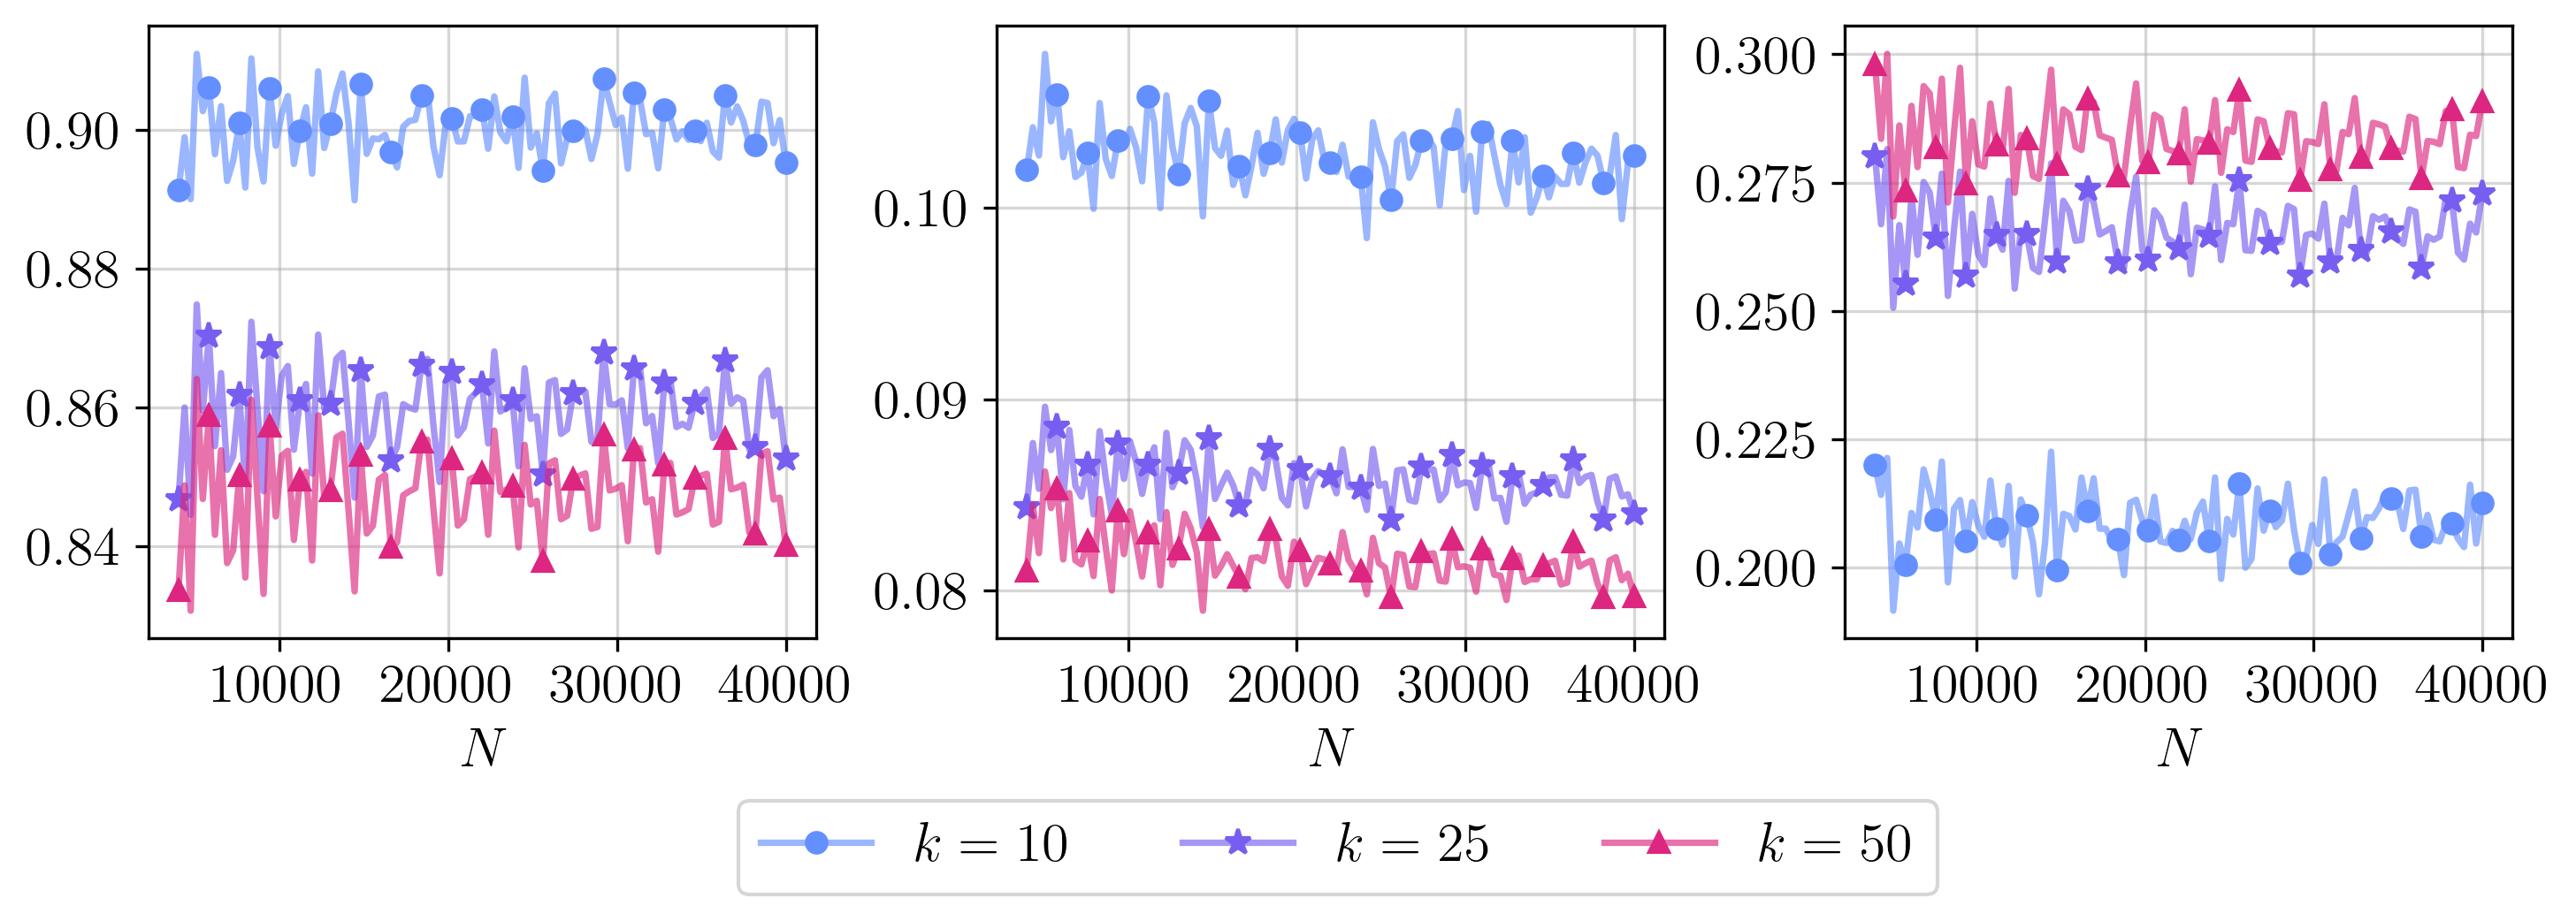
\includegraphics[width=1.0\textwidth]{mesh_resolution_effect.png}}
    \caption{The reconstruction error using rSVD with fixed $k$ and increasing mesh resolution $N$. Error measured using relative Euclidean norm (left), relative EMD (middle), and AUC-IoU (right) on Problem I. Values averaged over 5 repetitions.}
    \label{fig:mesh_resolution_effect}
\end{figure*}
In Figure~\ref{fig:mesh_resolution_effect}, we see that fixing the target rank $k$ and refining the mesh resolution $N$ does not decrease the Euclidean or AUC-IoU error. The EMD shows a slight decrease with $N$, likely because finer meshes produce smoother spatial transitions between neighboring mesh elements.

Although $\operatorname{rank}(K) = N_b$ grows with $N$, the target rank $k$ need not be adjusted: refining the mesh adds no new information about the source $f$.


\subsubsection{Approximation of singular values}\label{sec:approximation_of_singular_values}
\begin{table}[ht]
    \centering
    \begin{tabular}{c cccc}
    \toprule
    $p$
    & $\tilde \sigma_{10}  / \sigma_{10}$
    & $\tilde \sigma_{25}  / \sigma_{25}$
    & $\tilde \sigma_{50}  / \sigma_{50}$
    & $\tilde \sigma_{100} / \sigma_{100}$ \\
    \midrule
    $0$ & 1.000 & 0.993 & 0.962 & 0.566 \\
    
    \midrule
    $5$ & 1.000 & 0.995 & 0.969 & 0.668 \\

    \midrule
    $10$ & 1.000 & 0.995 & 0.973 & 0.724 \\
    \bottomrule
    \end{tabular}

    \caption{Ratio $\tilde \sigma_i / \sigma_i$ for selected singular values, across oversampling parameters $p=0,\,5,\,10$ using rSVD on $K$ (Algorithm~\ref{alg:discrete_rsvd}). Mean over 20 runs using Problem~I.}
    \label{tab:singular_values_comparison}
\end{table}
Table~\ref{tab:singular_values_comparison} shows that rSVD on $K$ underestimates the true singular values $\sigma_i$, with the bias increasing for higher-index values. Larger $p$ reduces the underestimation.

At $k = 50$, reconstruction errors were within 1\%-4\% of the exact Tikhonov solution in terms of Euclidean and AUC-IoU (Section~\ref{sec:target_rank_reconstruction}). At this rank with $p = 5$, the ratio $\tilde \sigma_{50}/\sigma_{50}$ is $0.969$: the underestimation is small where reconstruction quality is already high. If $\tilde \sigma_i \ll \sigma_i$, the approximated forward operator is more ill-posed than the true one, and reconstruction quality degrades. This is not the case at $k = 50$, where $\tilde \sigma_i / \sigma_i$ remains close to 1.


\subsubsection{Accuracy on noisy data}\label{sec:accuracy_on_noisy_data}
We measure the reconstruction error for the transformed weighted Tikhonov problem of Equation~\eqref{eq:transformed_discrete_inverse_problem}. We replace $y = K x$ with $\tilde y = y + \epsilon$, where $\epsilon_i \sim \mathcal{N}(0, 1)$ and $\tfrac{\| \epsilon \|}{\| y \|} = \delta$ with $\delta = 0.01$. The regularization parameter is set to $\lambda = \lambda_{\text{dp}}$, found using the discrepancy principle with safety factor $\nu_{\text{dp}} = 10$ (see Section~5.2 in Hansen \cite{hansen2010discrete}), so that $\lambda$ is selected independently for each method and rank.
\begin{table}[H]
    \centering
    \begin{tabular}{cc ccc}
    \toprule
    Problem & Method & Euclidean & EMD & AUC-IoU \\
    \midrule
    \multirow{2}{*}{I}
    & rSVD & 60 & 20 & 60 \\
    & tSVD & 60 & 20 & 80 \\
    
    \midrule
    \multirow{2}{*}{II}
    & rSVD & 50 & 20 & 65 \\
    & tSVD & 45 & 20 & 65 \\

    \midrule
    \multirow{2}{*}{III}
    & rSVD & 75 & 30 & $\ge$100 \\
    & tSVD & 85 & 30 & 95 \\
    \bottomrule
    \end{tabular}
    
\caption{The optimal target/truncation rank $k^*$ of rSVD/tSVD on noisy data using Problems~I, II, and III in terms of error metrics (mean over 50 runs): Euclidean norm, EMD, and AUC-IoU.}
\label{tab:noisy}
\end{table}
\begin{figure*}[htbp]
    \centerline{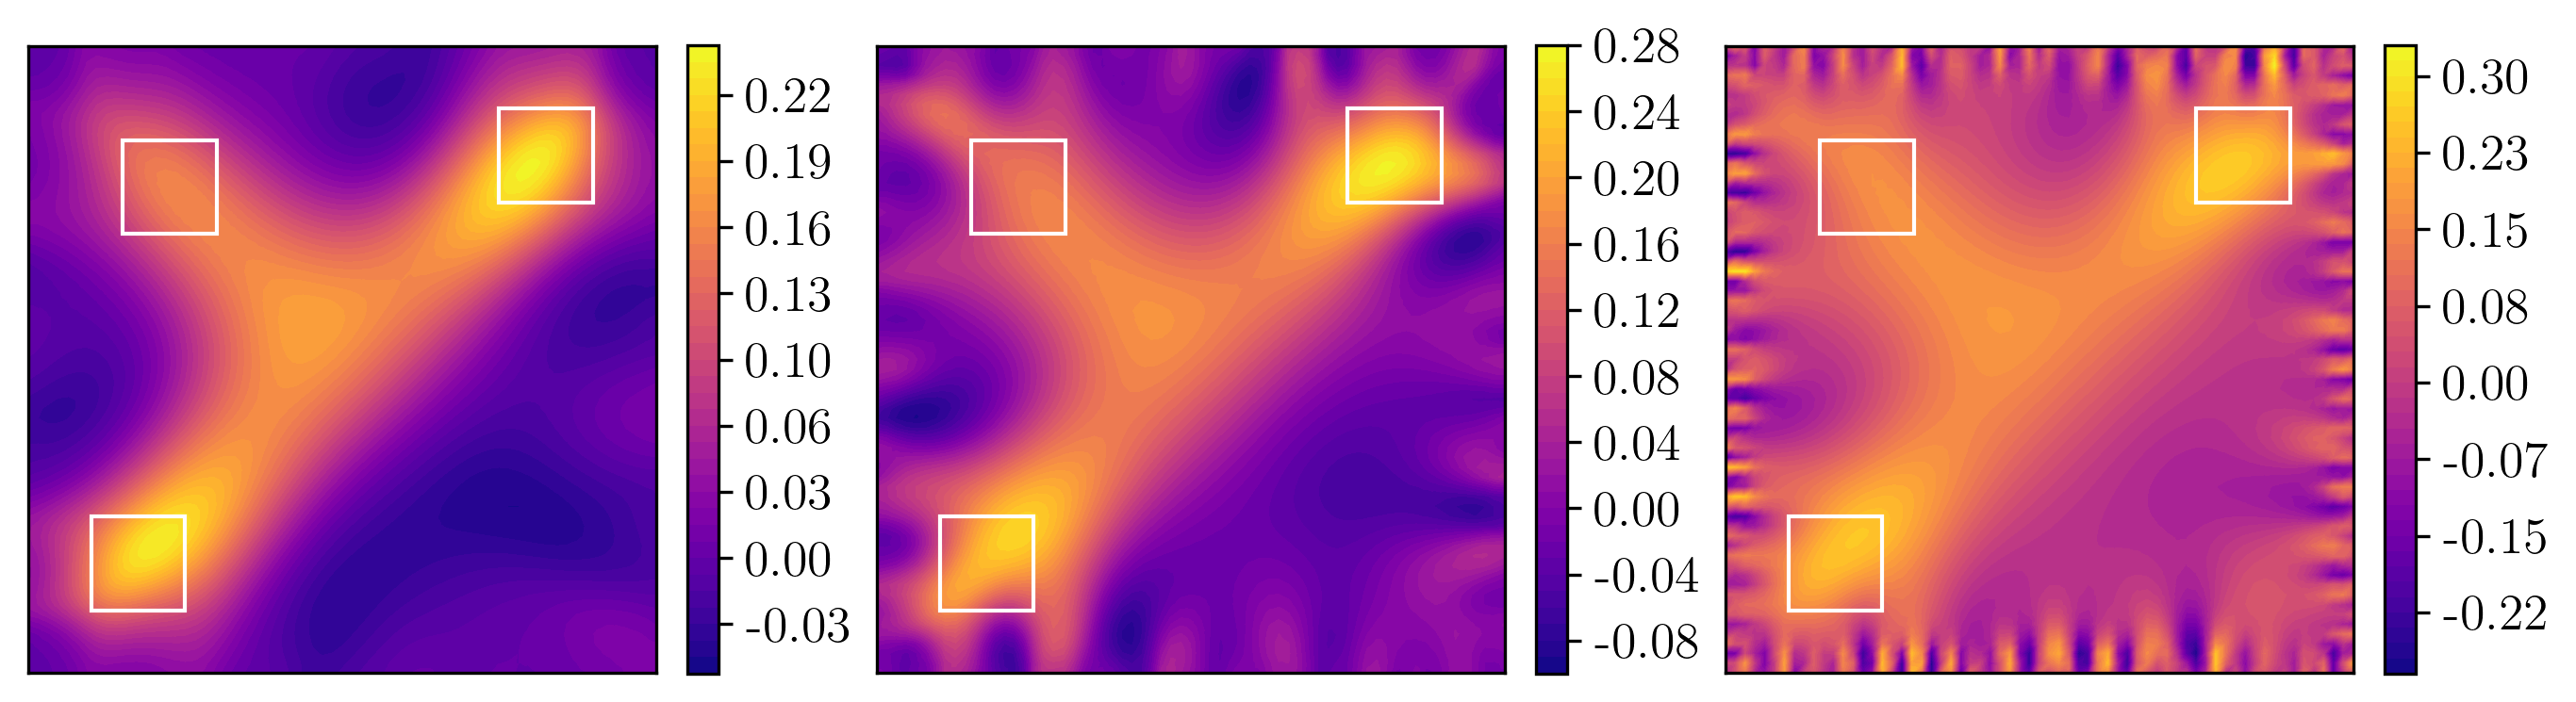
\includegraphics[width=1.0\textwidth]{reconstruction_noisy_problem.png}}
    \caption{Reconstructions (Problem~II) on a noisy problem using rSVD and $\lambda = \lambda_{\text{dp}}$ for target ranks 20 (left), 60 (middle), and 150 (right). True source locations outlined in white.}
    \label{fig:reconstruction_noisy_problem}
\end{figure*}

\begin{figure*}[htbp]
\centering

\begin{subfigure}{1.0\textwidth}
    \centering
    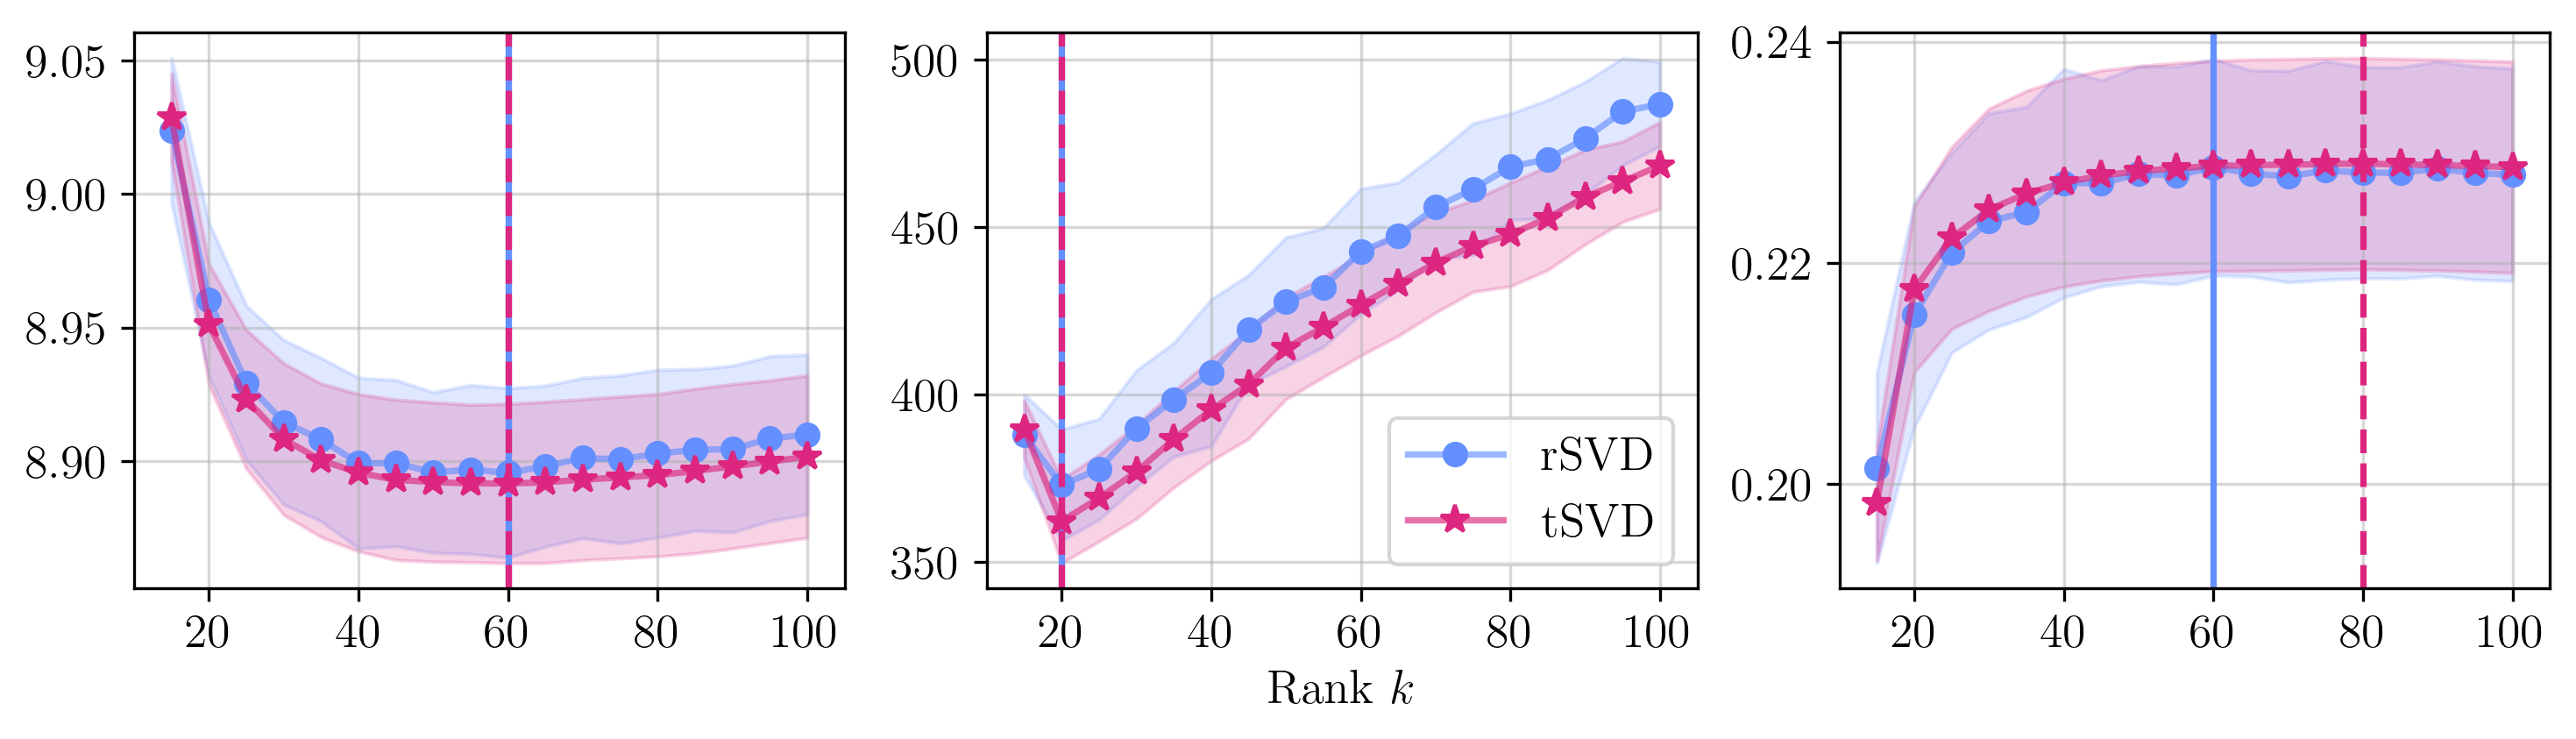
\includegraphics[width=\linewidth]{noisy_problem_I.png}
    \caption{Problem I.}
    \label{fig:noisy_problem_I}
\end{subfigure}

\vspace{0.5cm}

\begin{subfigure}{1.0\textwidth}
    \centering
    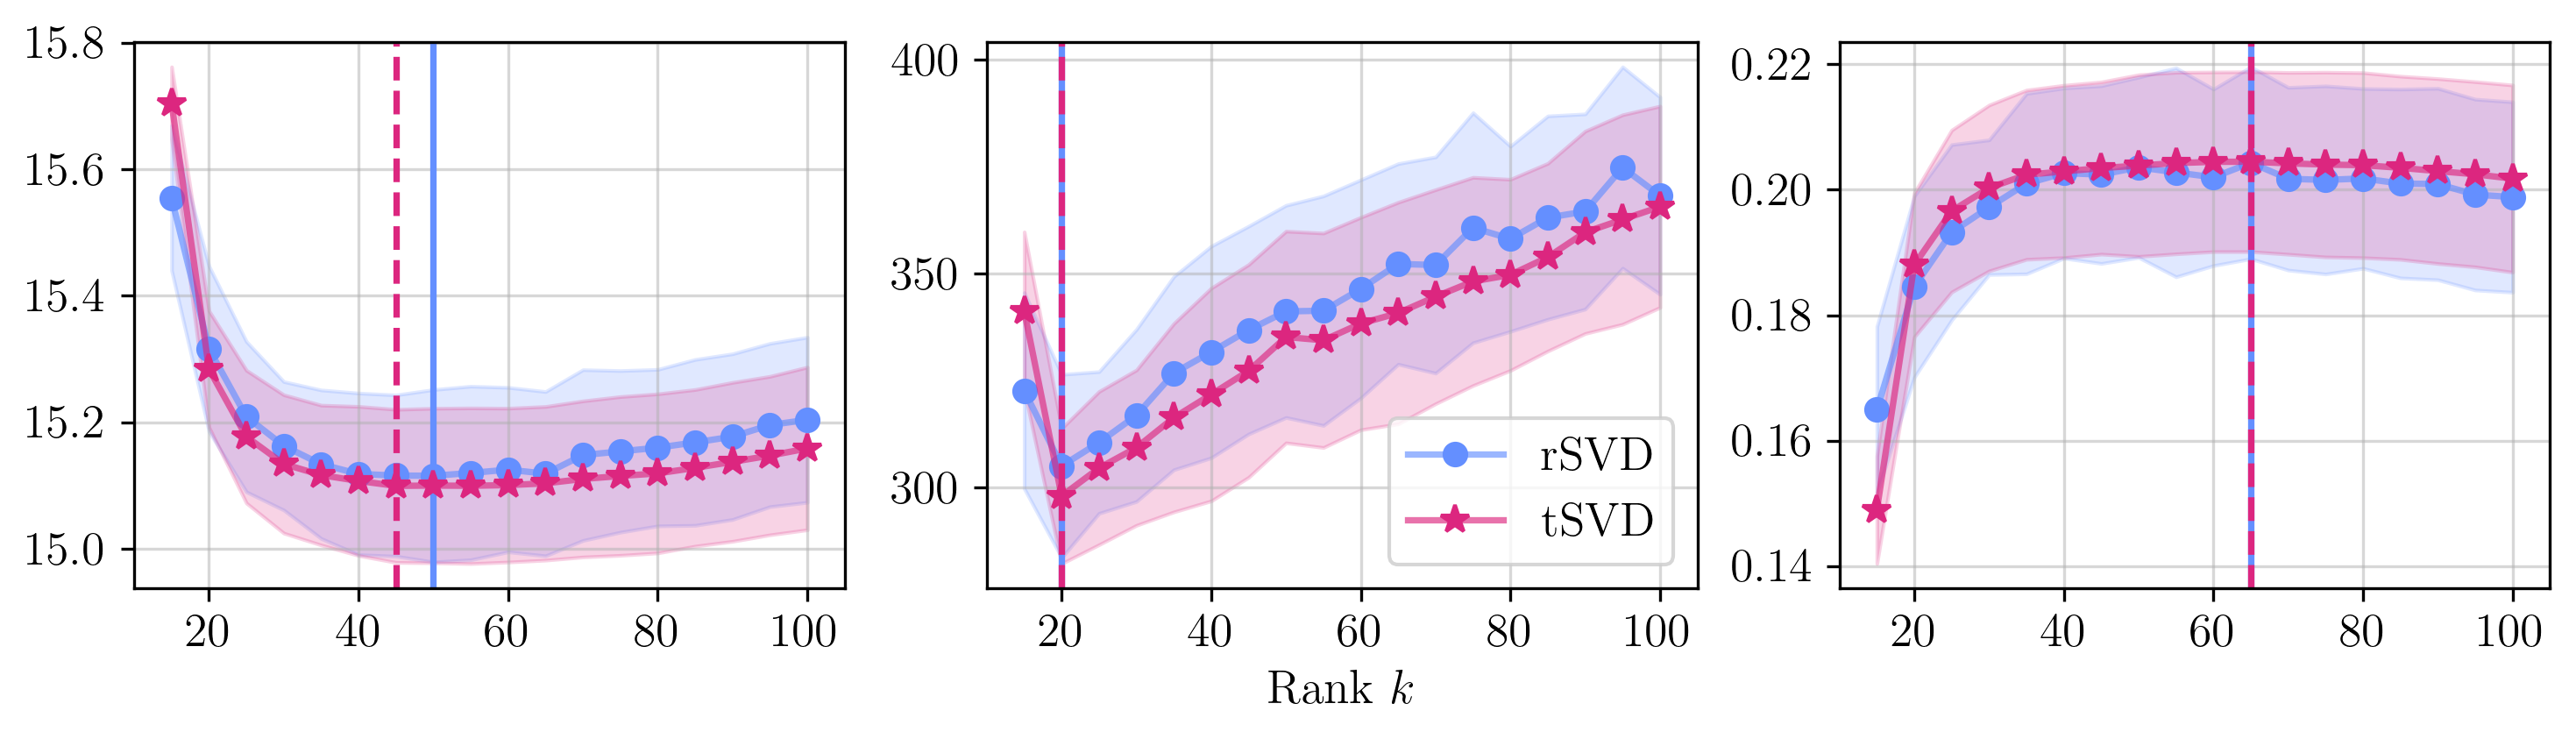
\includegraphics[width=\linewidth]{noisy_problem_II.png}
    \caption{Problem II.}
    \label{fig:noisy_problem_II}
\end{subfigure}

\vspace{0.5cm}

\begin{subfigure}{1.0\textwidth}
    \centering
    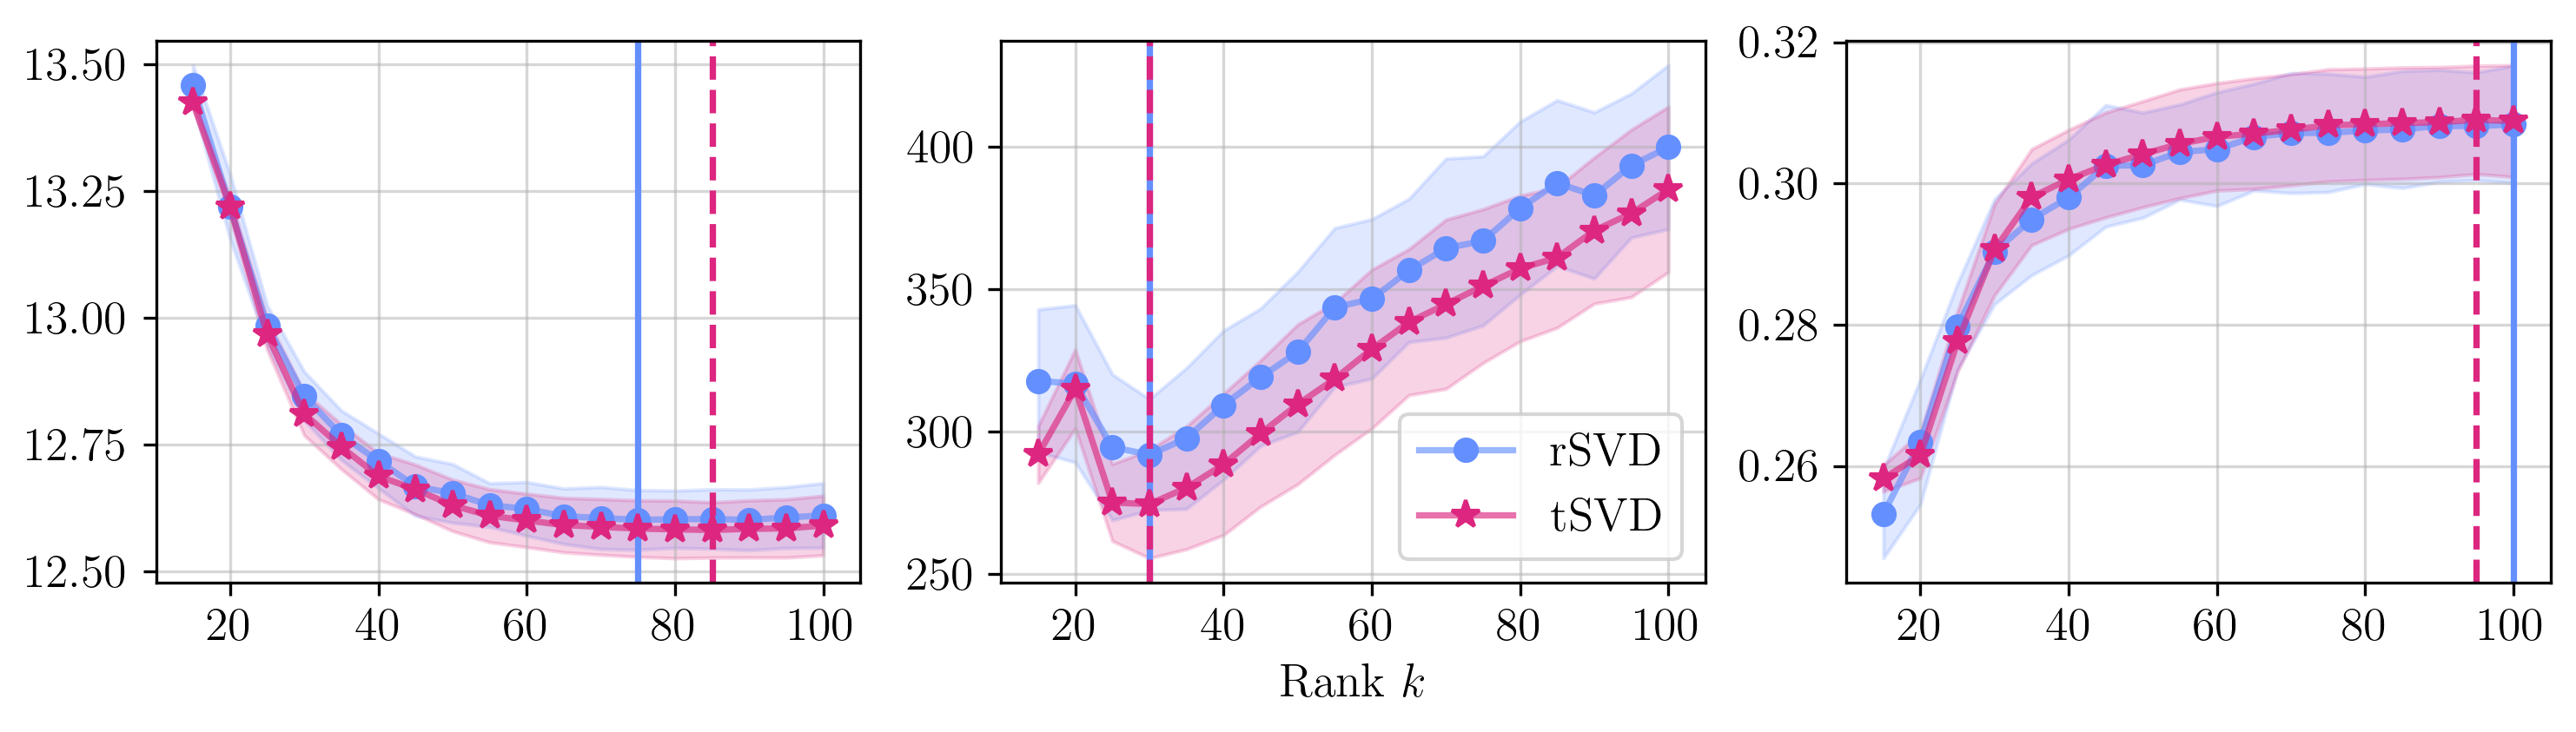
\includegraphics[width=\linewidth]{noisy_problem_III.png}
    \caption{Problem III.}
    \label{fig:noisy_problem_III}
\end{subfigure}

\caption{Reconstruction error using rSVD (Algorithm~\ref{alg:discrete_rsvd}) and tSVD to approximate $K$ and $W$ at different ranks on noisy problems. Error measured in: Euclidean norm (left), EMD (middle), AUC-IoU (right). Average over 50 runs with $\pm 1$ standard deviation. Optimal rank marked with vertical solid and dashed lines for rSVD and tSVD, respectively.}
\label{fig:noisy_problem}
\end{figure*}

Figure~\ref{fig:noisy_problem} and Table~\ref{tab:noisy} report reconstruction error and optimal ranks for rSVD (Algorithm~\ref{alg:discrete_rsvd}) and tSVD (Equation~\eqref{eq:tsvd}) on the noisy problem. Figure~\ref{fig:reconstruction_noisy_problem} illustrates how a target rank that is too high includes noise in the reconstruction.

In terms of Euclidean error, the optimal rank is between 50 and 75 for rSVD, and 45 and 85 for tSVD. The EMD is more sensitive to higher ranks which include more noise (Figure~\ref{fig:reconstruction_noisy_problem}), and the optimal rank for EMD is between 20 and 30 for both methods. For AUC-IoU, optimal ranks are between 60 and 65 for rSVD, and between 65 and 95 for tSVD, except for Problem~III with rSVD where the optimal rank exceeds the tested range.

At their respective optimal ranks, rSVD and tSVD give nearly identical Euclidean errors and AUC-IoU scores across the three problems, with differences below 0.25\%. The largest gap is in EMD: tSVD achieves 2.35\% to 6.33\% lower EMD, with the largest difference on Problem~III.

%%%%%%%%%%%%%%%%%%%%%%%%%%%%%%%%%%%%%%%%%%%%%%%%%%%%%%%%%%%%%
% Dynamical Low-Rank Approximation using (Preconditioned) Conjugate Gradient Part 
%%%%%%%%%%%%%%%%%%%%%%%%%%%%%%%%%%%%%%%%%%%%%%%%%%%%%%%%%%%%%
\subsection{Dynamical low-rank approximation}
Unless stated otherwise, all experiments use a rank-$50$ rSVD approximation of $K$ and $W$ (Algorithm~\ref{alg:discrete_rsvd}, $p = 5$, standard Gaussian test vectors $\psi_i$) to form $\Phi$, its gradient, and its Hessian (Section~\ref{sec:application_to_inverse_problem}), on which Algorithm~\ref{alg:DLRA-CG} is applied to find a low-rank solution.

We write $X^* \in \mathbb{R}^{n \times n}$ for the matrix form of the true source, and $N_r$ for the restart period of restarted DLRA-CG (Section~\ref{sec:restarted_cg}). Convergence is measured by the relative reconstruction error
\begin{equation*}
    e^{(i)} = \frac{\|X^{(i)} - X^*\|_F}{\|X^{(0)} - X^*\|_F},
\end{equation*}
which equals 1 at initialization and decreases toward 0 as the iterates approach $X^*$. Unless stated otherwise, $X^{(0)}$ has entries drawn uniformly from $[0,\,10^{-3}]$.


\subsubsection{Rate of convergence}\label{sec:rate_of_convergence}
\begin{figure*}[thbp]
    \centerline{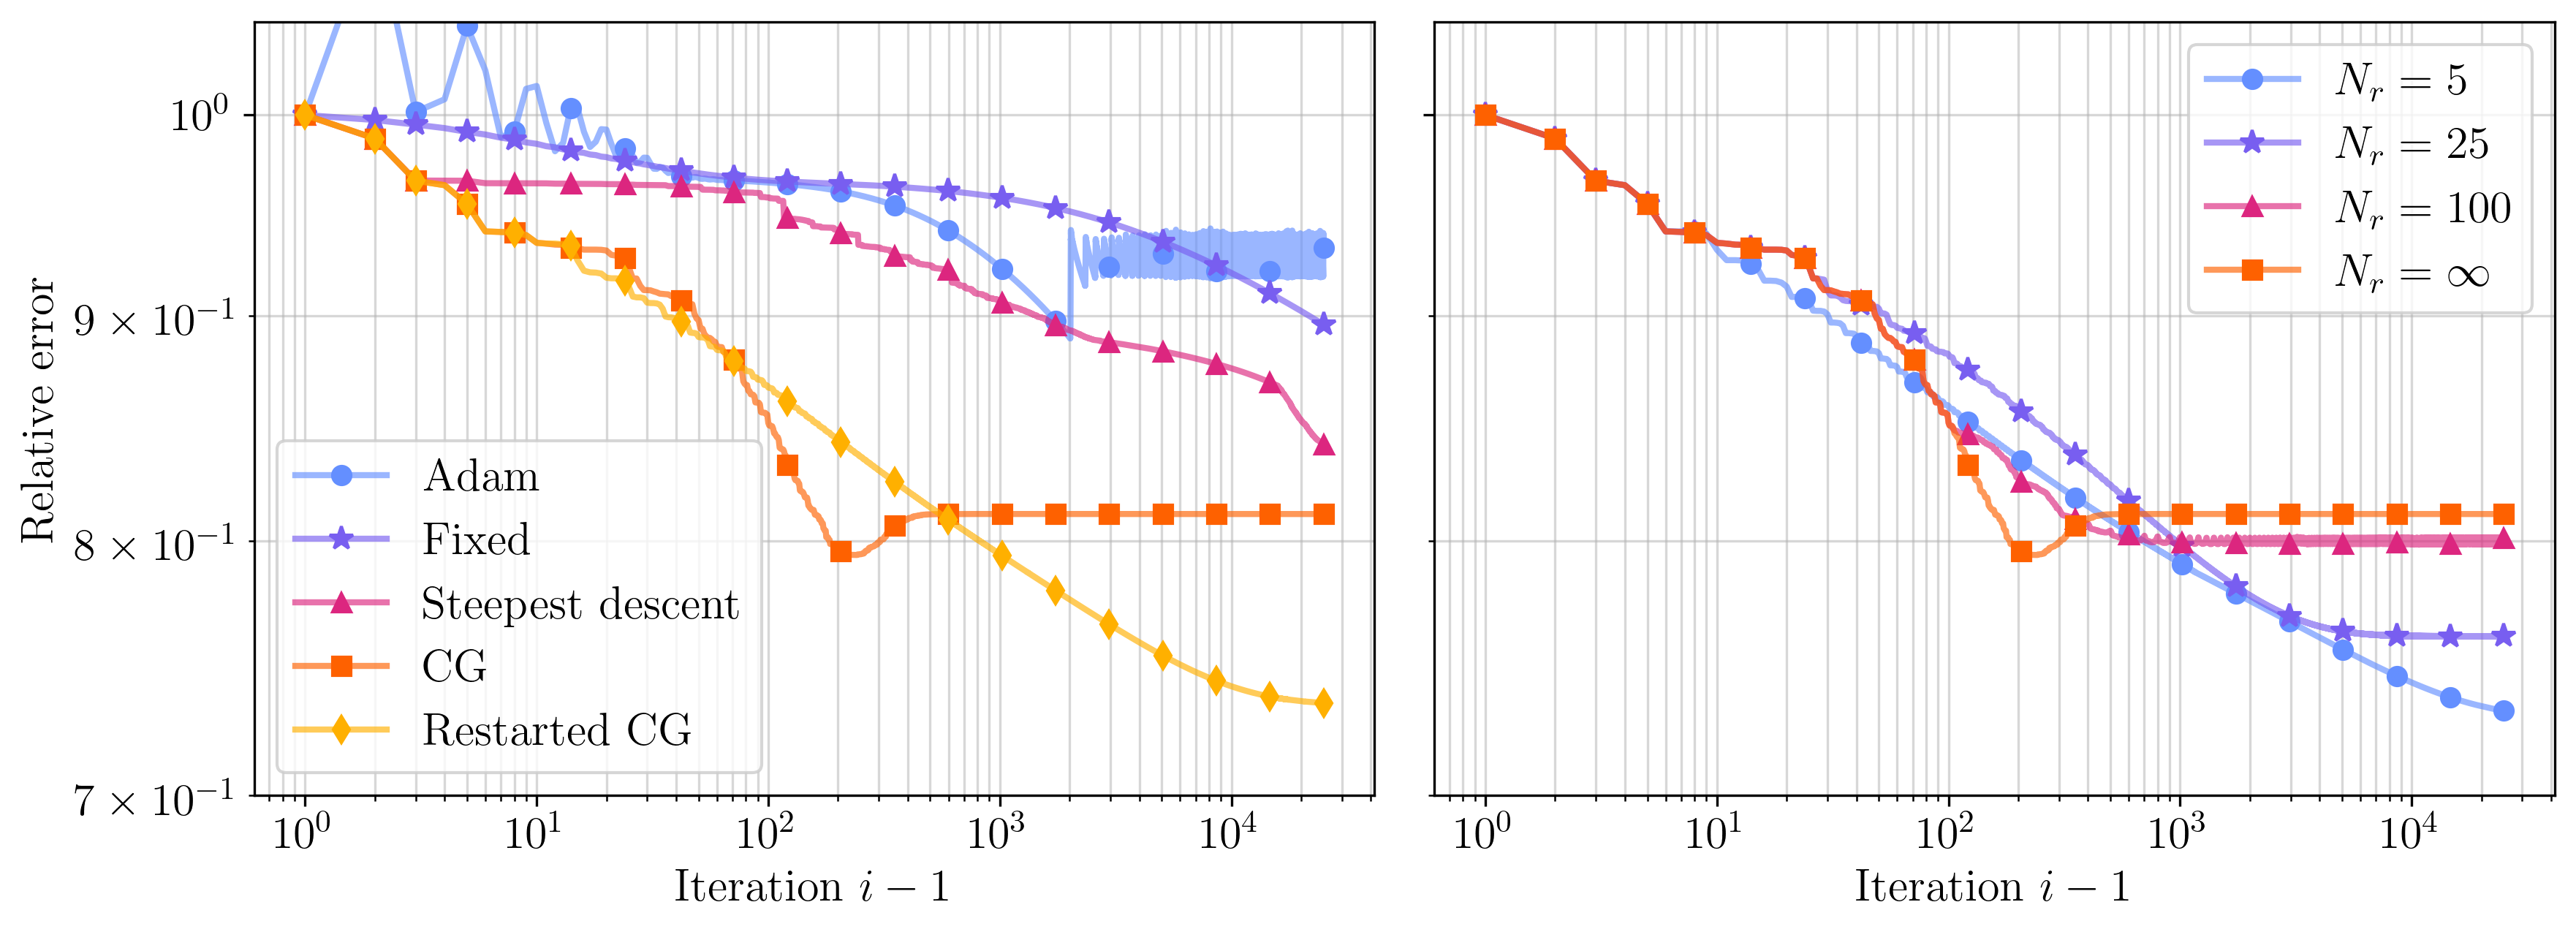
\includegraphics[width=1.0\textwidth]{number_of_iterations.png}}
    \caption{Relative reconstruction error $e^{(i)}$ versus iteration count.
    Left: three DLRA step-size rules (Adam, fixed step, steepest descent) and DLRA-CG (with and without restarting, using $N_r = 10$ for restarting).
    Right: DLRA using CG with different restart periods $N_r$, with $N_r = \infty$ being no restarting.}
    \label{fig:number_of_iterations}
\end{figure*}
\begin{table}[!ht]
\centering
\begin{tabular}{lrrrr}
\hline
Method & $< 0.90$ & $< 0.85$ & $< 0.80$ & $< 0.75$ \\
\hline
Adam                   & 1665 & \texttt{-} & \texttt{-} & \texttt{-} \\
Fixed                  & 21751 & \texttt{-} & \texttt{-} & \texttt{-} \\
Steepest descent       & 1449 & 20916 & \texttt{-} & \texttt{-} \\
DLRA-CG                & 48 & 100 & 184 & \texttt{-} \\
Restarted DLRA-CG      & 35 & 165 & 816 & 5941 \\
\hline
\end{tabular}
\caption{Number of iterations to reach a given relative reconstruction error $e^{(i)}$ for each method (Problem~I), where \texttt{-} indicates the threshold was not reached. For restarted CG, $N_r = 10$ was used.}
\label{tab:convergence_iterations}
\end{table}
Figure~\ref{fig:number_of_iterations} compares the reconstruction error per iteration for three DLRA step-size rules (Algorithm~\ref{alg:dlra}) and DLRA-CG (Algorithm~\ref{alg:DLRA-CG}), with and without restarting. The right panel shows the effect of the restart period $N_r$ on the convergence of DLRA-CG.

DLRA-CG reaches the lowest error fastest but then the error rises, showing a form of semi-convergence, as the full-rank trajectory $Y^{(i)}$ drifts away from $X^{(i)}$ (Section~\ref{sec:restarted_cg}). Restarted DLRA-CG (with $N_r = 10$) avoids this by periodically correcting the CG recurrence to $X^{(i)}$, at the cost of slower convergence, but converges faster than the three DLRA step-size rules, which all fail to converge within $25{,}000$ iterations (and the Adam
rule gets stuck).

A smaller $N_r$ slows convergence but drives the error lower, and for larger $N_r$, the semi-convergent behavior of DLRA-CG re-appears. Table~\ref{tab:convergence_iterations} shows the iteration count to reach selected error thresholds. DLRA-CG reaches a relative error of $0.9$ in 48 iterations, and restarted DLRA-CG takes 35 iterations. The step-size rules Adam, fixed, and steepest descent reach this threshold in 1665, 21751, and 1449 iterations. To reach a threshold of $0.85$, DLRA-CG takes 100 iterations and restarted DLRA-CG takes 165. At $0.75$, only restarted DLRA-CG succeeds, requiring 5941 iterations.

Per-iteration compute times are similar across all methods ($0.5$-$0.7$ ms), so the iteration counts in Table~\ref{tab:convergence_iterations} translate directly to runtime. At $e^{(i)} < 0.85$, DLRA-CG is approximately $210$ times faster than steepest descent.


\subsubsection{Quality of the low-rank solutions}\label{sec:quality_of_the_low_rank_solutions}
\begin{figure*}[htbp]
\centering

\begin{subfigure}{1.0\textwidth}
    \centering
    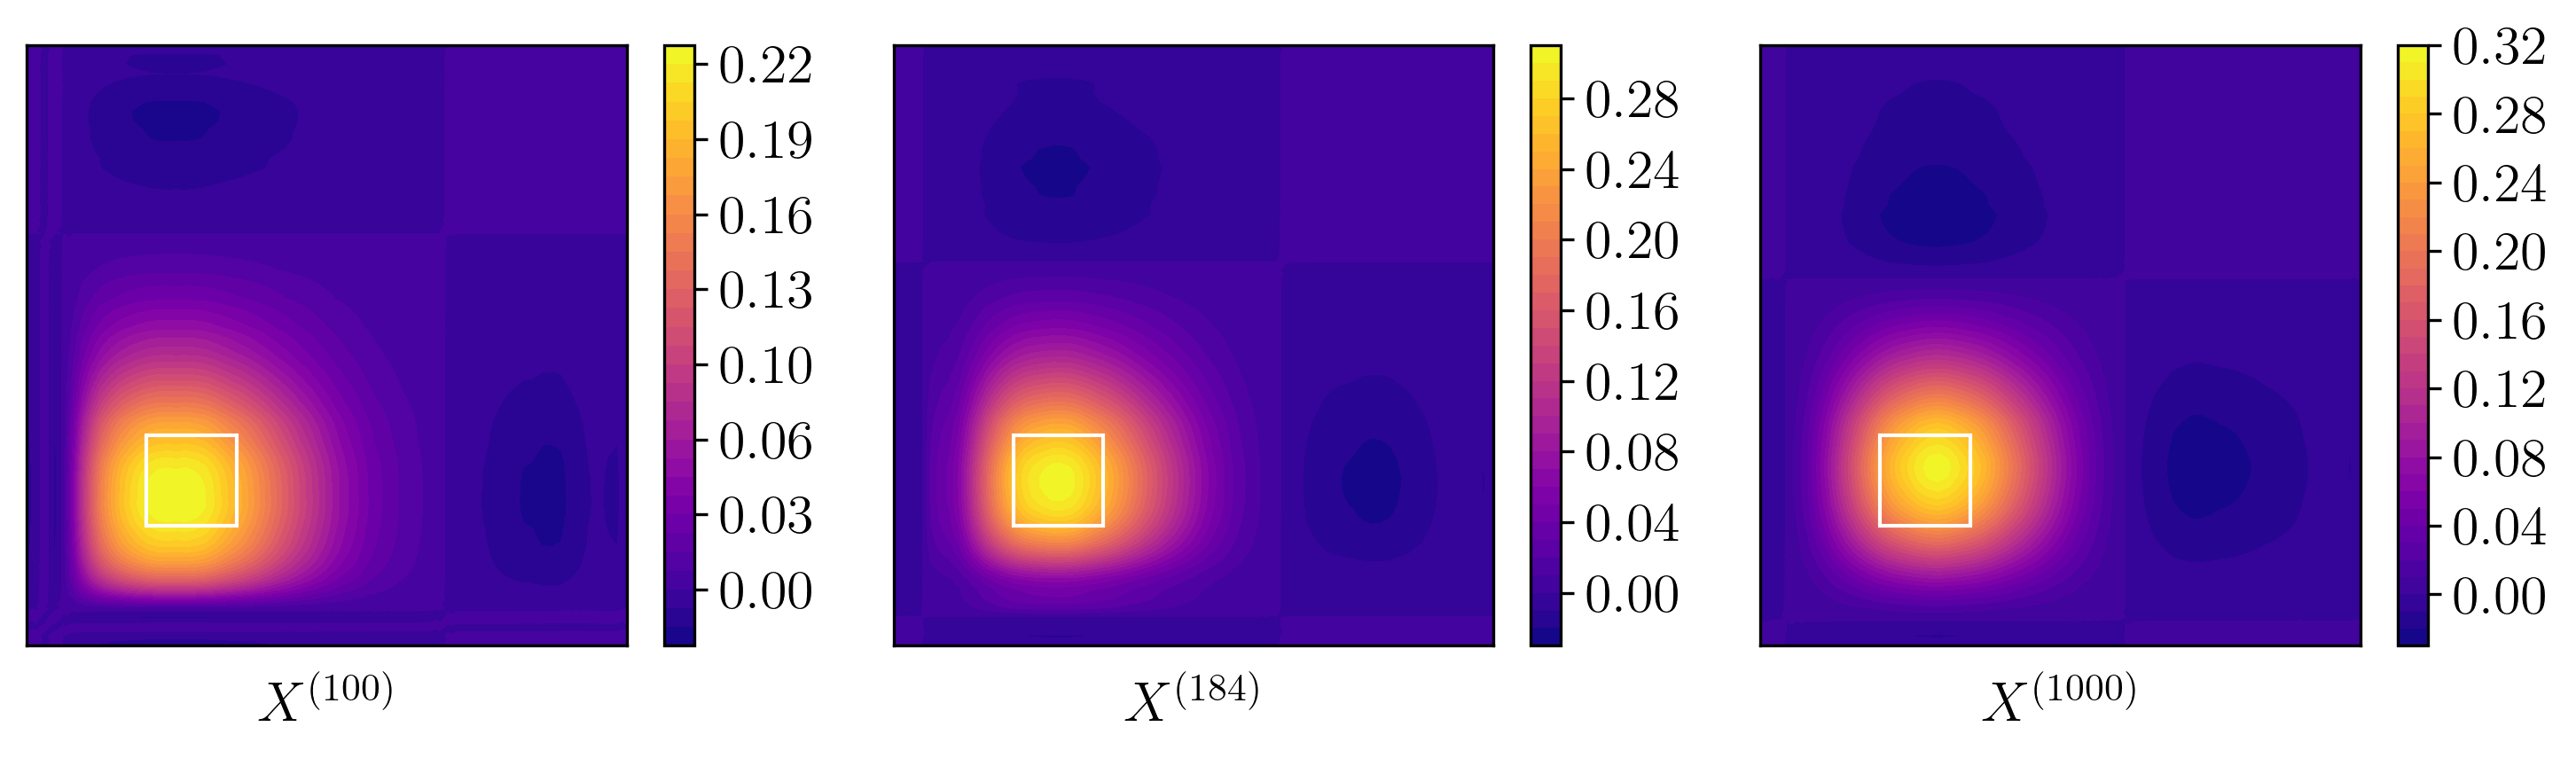
\includegraphics[width=\linewidth]{low_rank_convergence_I.png}
    \caption{Problem I and $r = 1$. $e^{(i)}$ from left to right: $0.85$, $0.80$, $0.81$.}
    \label{fig:low_rank_convergence_I}
\end{subfigure}

\vspace{0.5cm}

\begin{subfigure}{1.0\textwidth}
    \centering
    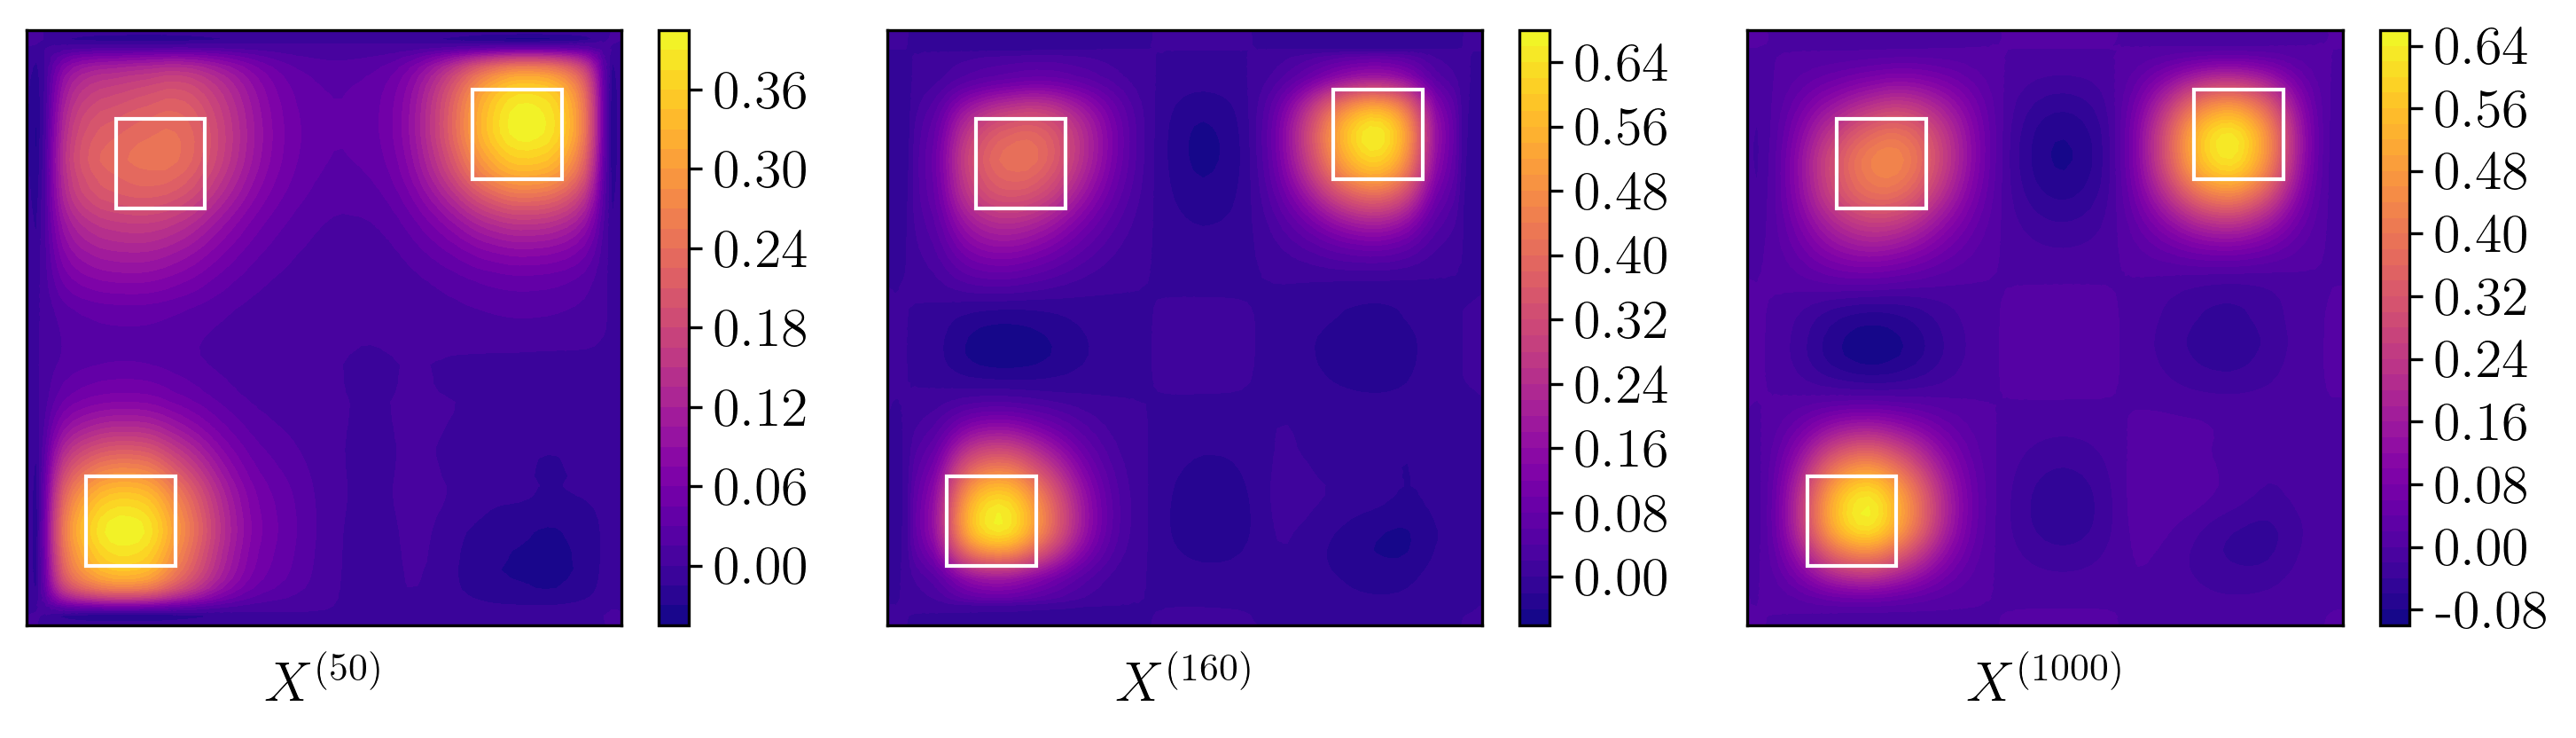
\includegraphics[width=\linewidth]{low_rank_convergence_II.png}
    \caption{Problem II and $r = 2$. $e^{(i)}$ from left to right: $0.78$, $0.65$, $0.67$.}
    \label{fig:low_rank_convergence_II}
\end{subfigure}

\caption{Iterates $X^{(i)}$ of Algorithm~\ref{alg:DLRA-CG} (no restarting) at three stages of the same run: an early iterate before the error minimum (left), the iterate at minimum reconstruction error (middle), and a converged iterate at which the error has risen above the minimum due to semi-convergence (right). True source outlined in white.}
\label{fig:low_rank_convergence}
\end{figure*}

\begin{figure*}[htbp]
    \centerline{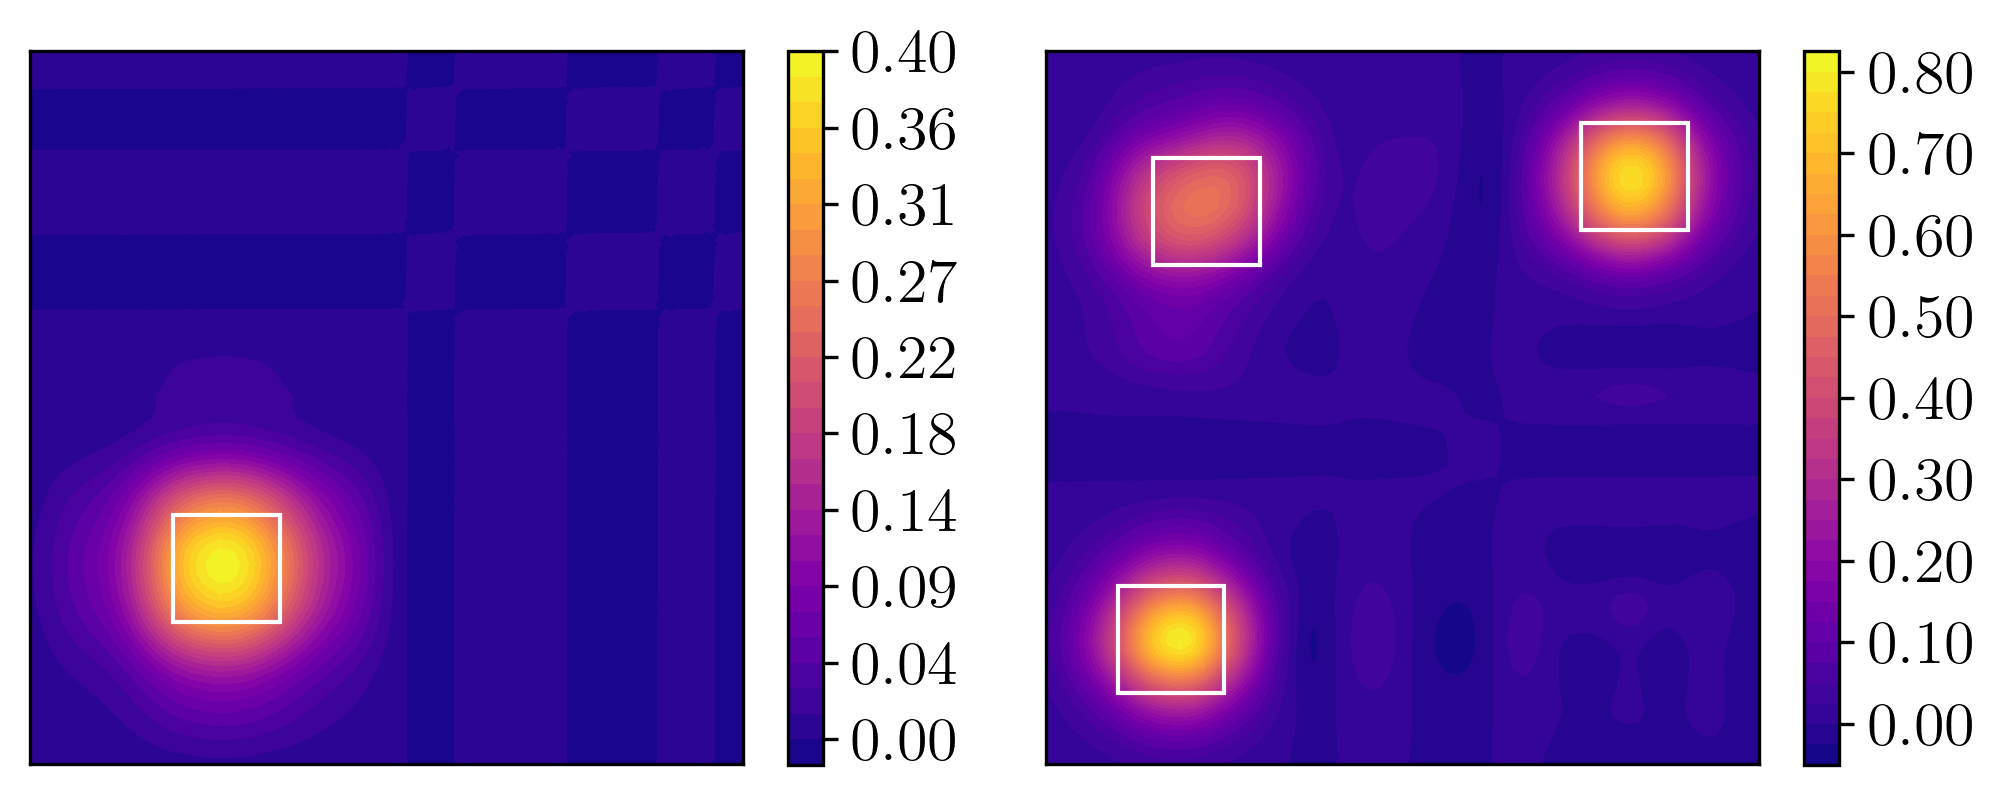
\includegraphics[width=0.65\textwidth]{low_rank_restarted_CG.png}}
    \caption{Reconstructions using restarted CG ($N_r = 10$) with $25{,}000$ iterations (run until convergence), with same respective $X^{(0)}$s as in Figure~\ref{fig:low_rank_convergence}. Left: Problem~I, rank 1, $e^{(i)}=0.73$. Right: Problem~II, rank 2, $e^{(i)}=0.63$. True source outlined in white.}
    \label{fig:low_rank_restarted_cg}
\end{figure*}

DLRA-CG shows semi-convergence: the iterates initially approach the true source, but start to move away from the optimal solution when $X^{(i)}$ and $Y^{(i)}$ drift apart (Section~\ref{sec:restarted_cg}). Figure~\ref{fig:low_rank_convergence} shows the difference between the minimum reconstruction iterate and the converged iterate. In both Problems~I and II, the converged iterate (right panels) shows a slight inward shift of the source positions, while the minimum-error iterate (middle panels) correctly reproduces the source locations. The early iterate (left panels) has not yet localized the sources.

Compared to the full-rank solutions of Section~\ref{sec:target_rank_reconstruction}, which have smoothing pulled toward the interior, the low-rank solutions are more uniformly smoothed with no such tail. For Problem~I, this creates a circular source, and for Problem~II, this results in cleanly separated sources (in Figure~\ref{fig:test_problem_II} they were connected). Additionally, at $k = 50$, the peak amplitudes are $0.28$ (rank-1 DLRA-CG) versus $0.26$ (full-rank rSVD) for Problem~I, and $0.64$ versus $0.48$ for Problem~II, where the upper-left source is weaker in the rank-2 solution. The true source amplitude is 1.0 (Figure~\ref{fig:problem_illustration}). The low-amplitude noise in the full-rank rSVD solution is replaced by a checker-like pattern of similar amplitude.

Restarted DLRA-CG ($N_r = 10$) achieves a lower relative error than DLRA-CG without restarting (Figure~\ref{fig:number_of_iterations}, left). The converged solutions in Figure~\ref{fig:low_rank_restarted_cg} are correctly located and less diffuse, with peak amplitudes of $0.40$ and $0.80$ for Problems~I and II, closer to the true amplitude of $1.0$ than both the full-rank rSVD Tikhonov solutions and the solutions without restarting.


\subsubsection{Effect of rank on reconstructions}\label{sec:effect_of_rank_on_reconstructions}
\begin{figure*}[htbp]
\centering

\begin{subfigure}{1.0\textwidth}
    \centering
    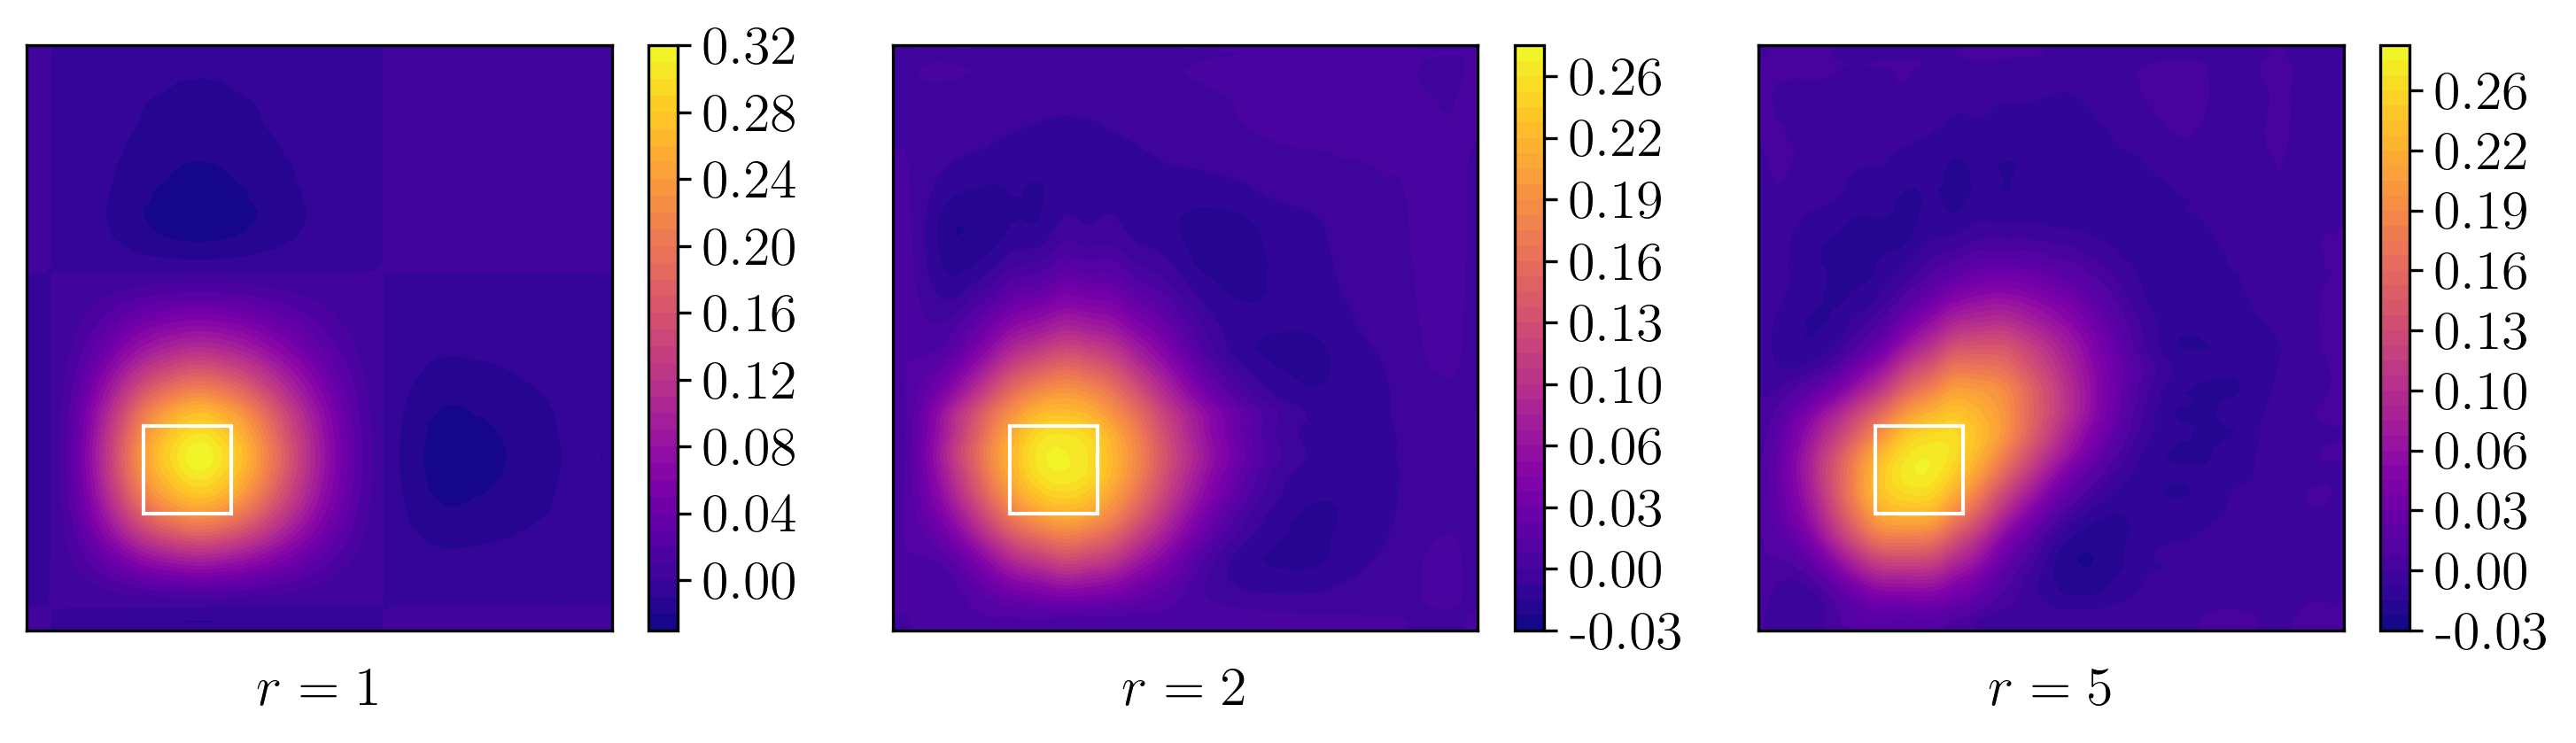
\includegraphics[width=\linewidth]{low_rank_different_r_I.png}
    \caption{Problem I: The rank-1 solution (left) gives the best reconstruction. $e^{(i)}$ from left to right: $0.81$, $0.83$, $0.84$.}
    \label{fig:low_rank_different_r_I}
\end{subfigure}

\vspace{0.5cm}

\begin{subfigure}{1.0\textwidth}
    \centering
    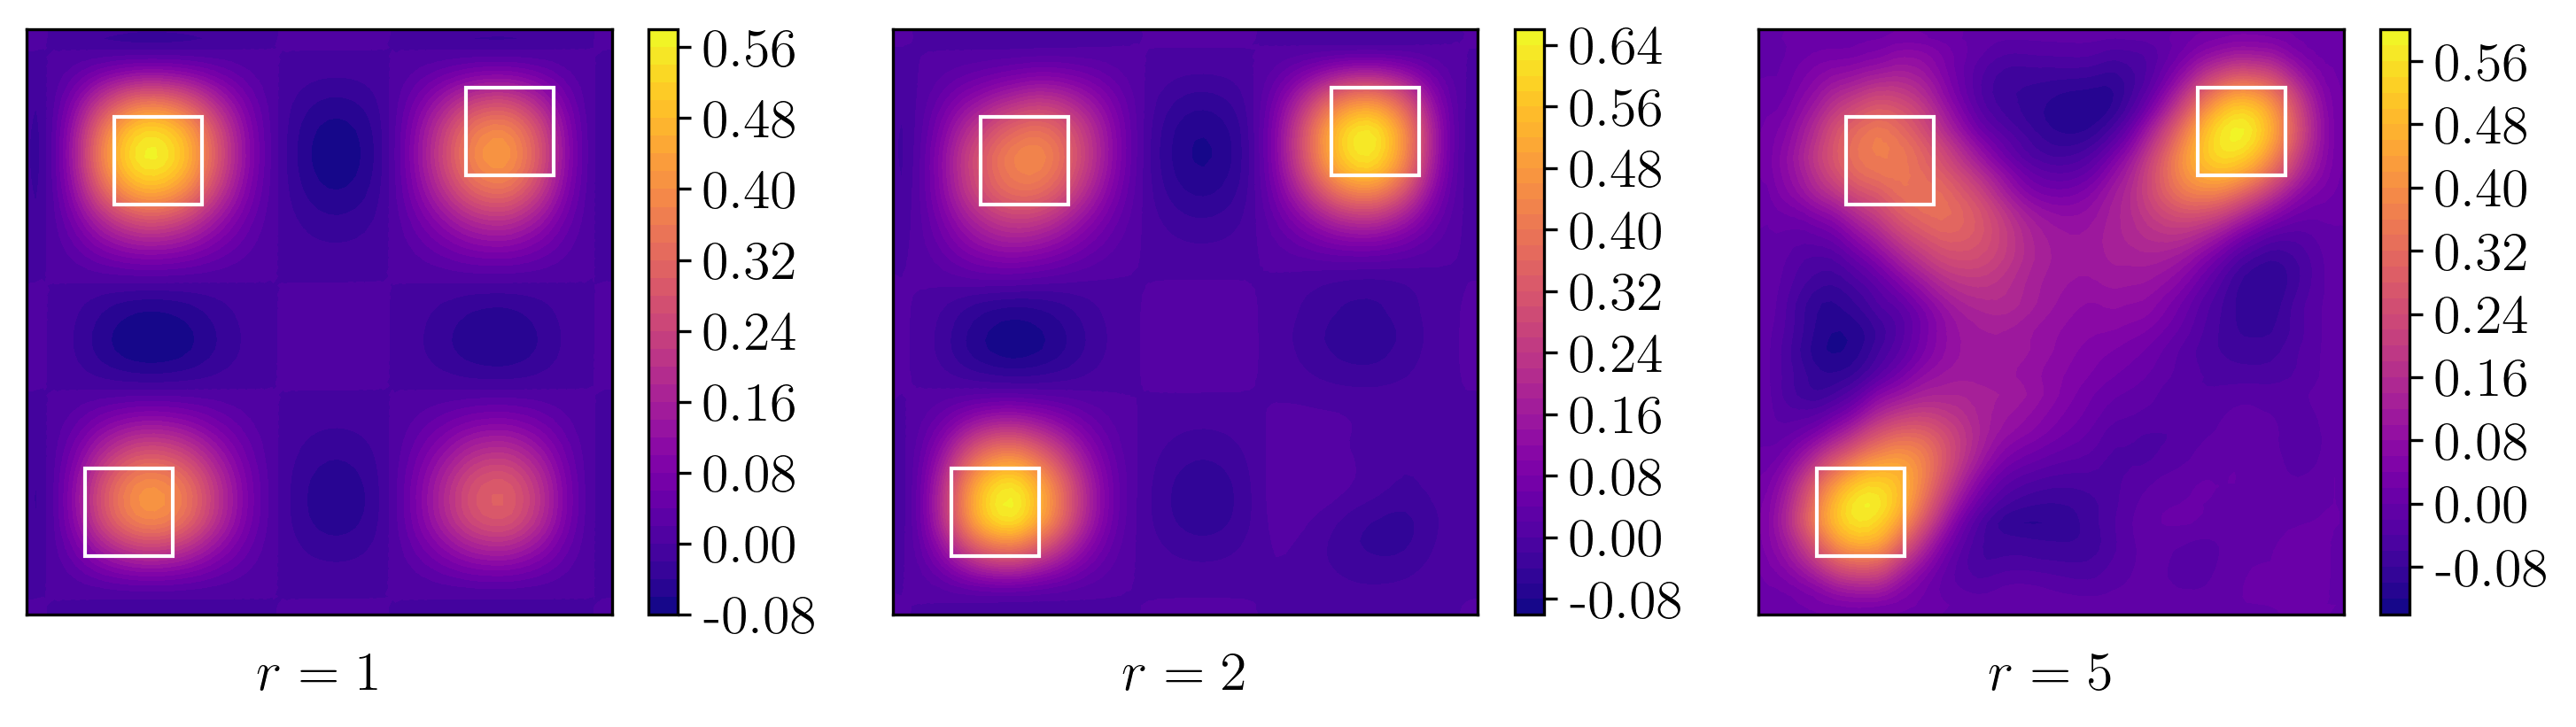
\includegraphics[width=\linewidth]{low_rank_different_r_II.png}
    \caption{Problem II: The rank-1 solution (left) places an additional source at bottom right, where no true source exists; the rank-2 solution gives the best reconstruction (middle). $e^{(i)}$ from left to right: $0.75$, $0.67$, $0.73$.}
    \label{fig:low_rank_different_r_II}
\end{subfigure}

\caption{Low-rank solutions of Algorithm~\ref{alg:DLRA-CG} (no restarting) at selected ranks $r = 1$ (left), $r = 2$ (middle), and $r = 5$ (right). True source outlined in white.}
\label{fig:low_rank_different_r}
\end{figure*}

\begin{figure*}[htbp]
\centering

\begin{subfigure}{1.0\textwidth}
    \centering
    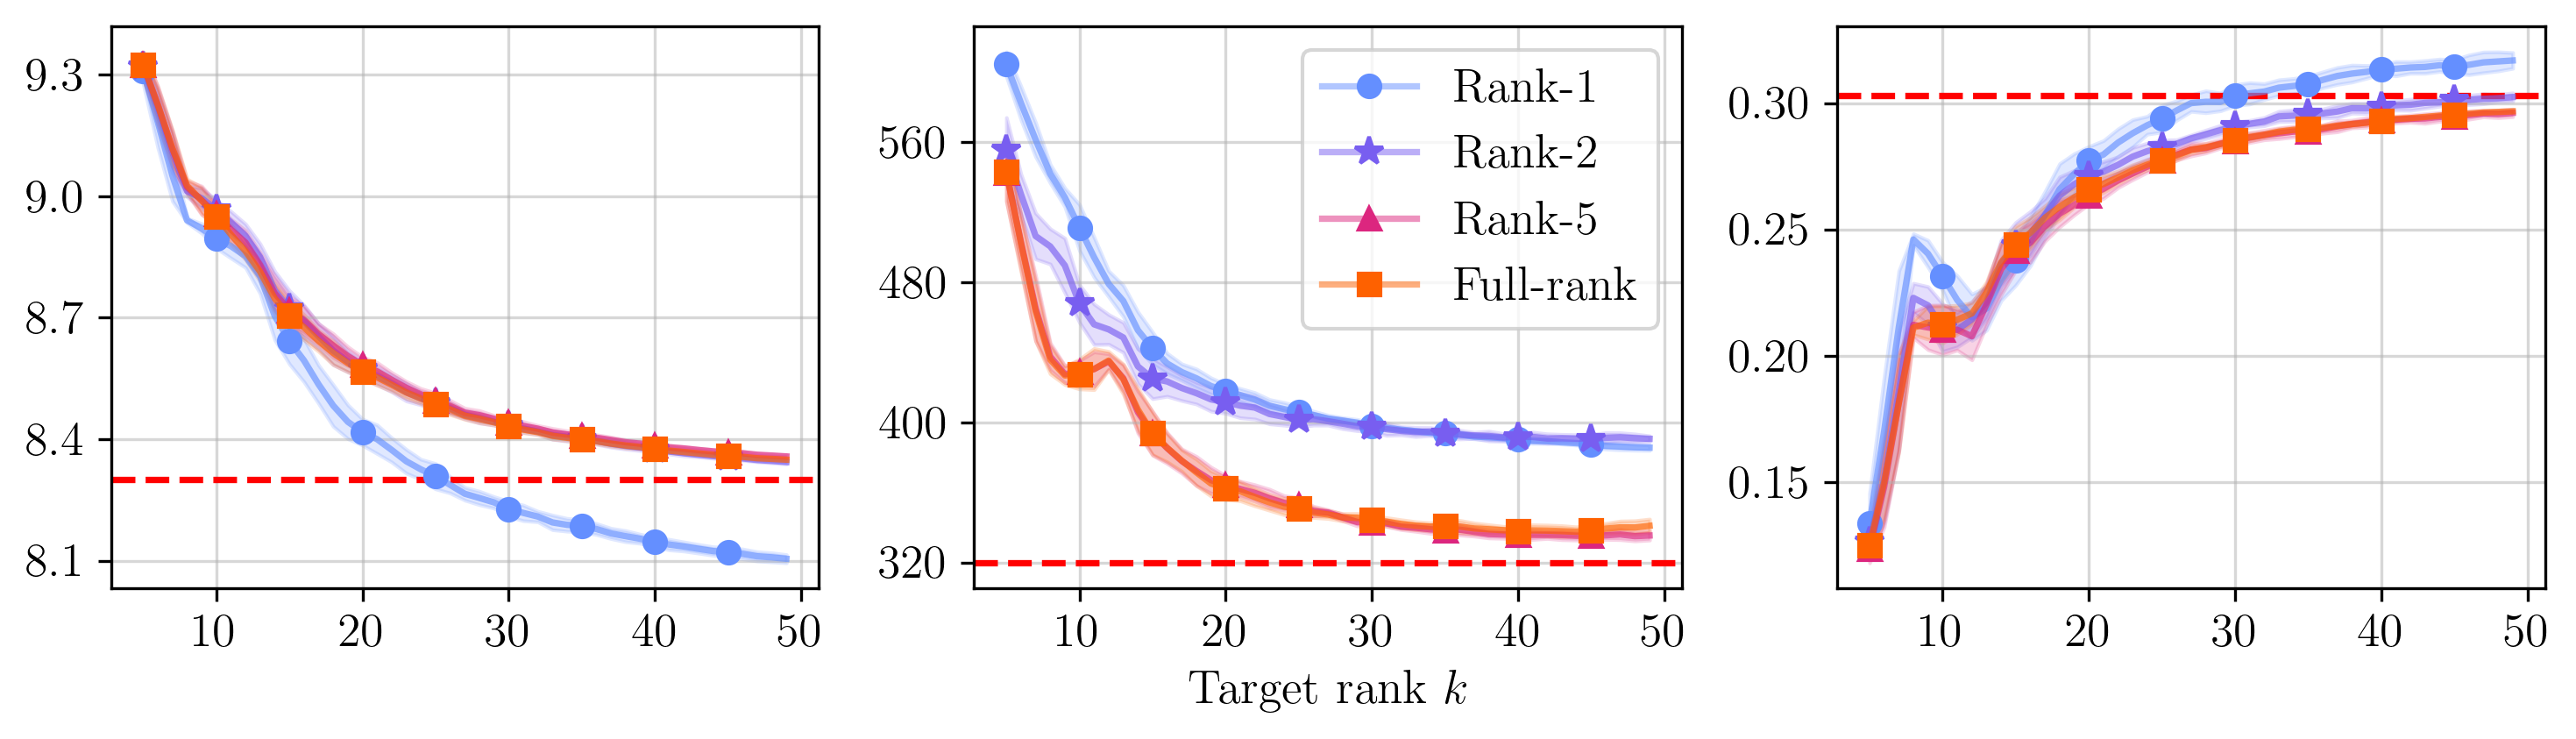
\includegraphics[width=\linewidth]{low_rank_solution_error_I.png}
    \caption{Problem I.}
    \label{fig:low_rank_solution_error_I}
\end{subfigure}

\vspace{0.5cm}

\begin{subfigure}{1.0\textwidth}
    \centering
    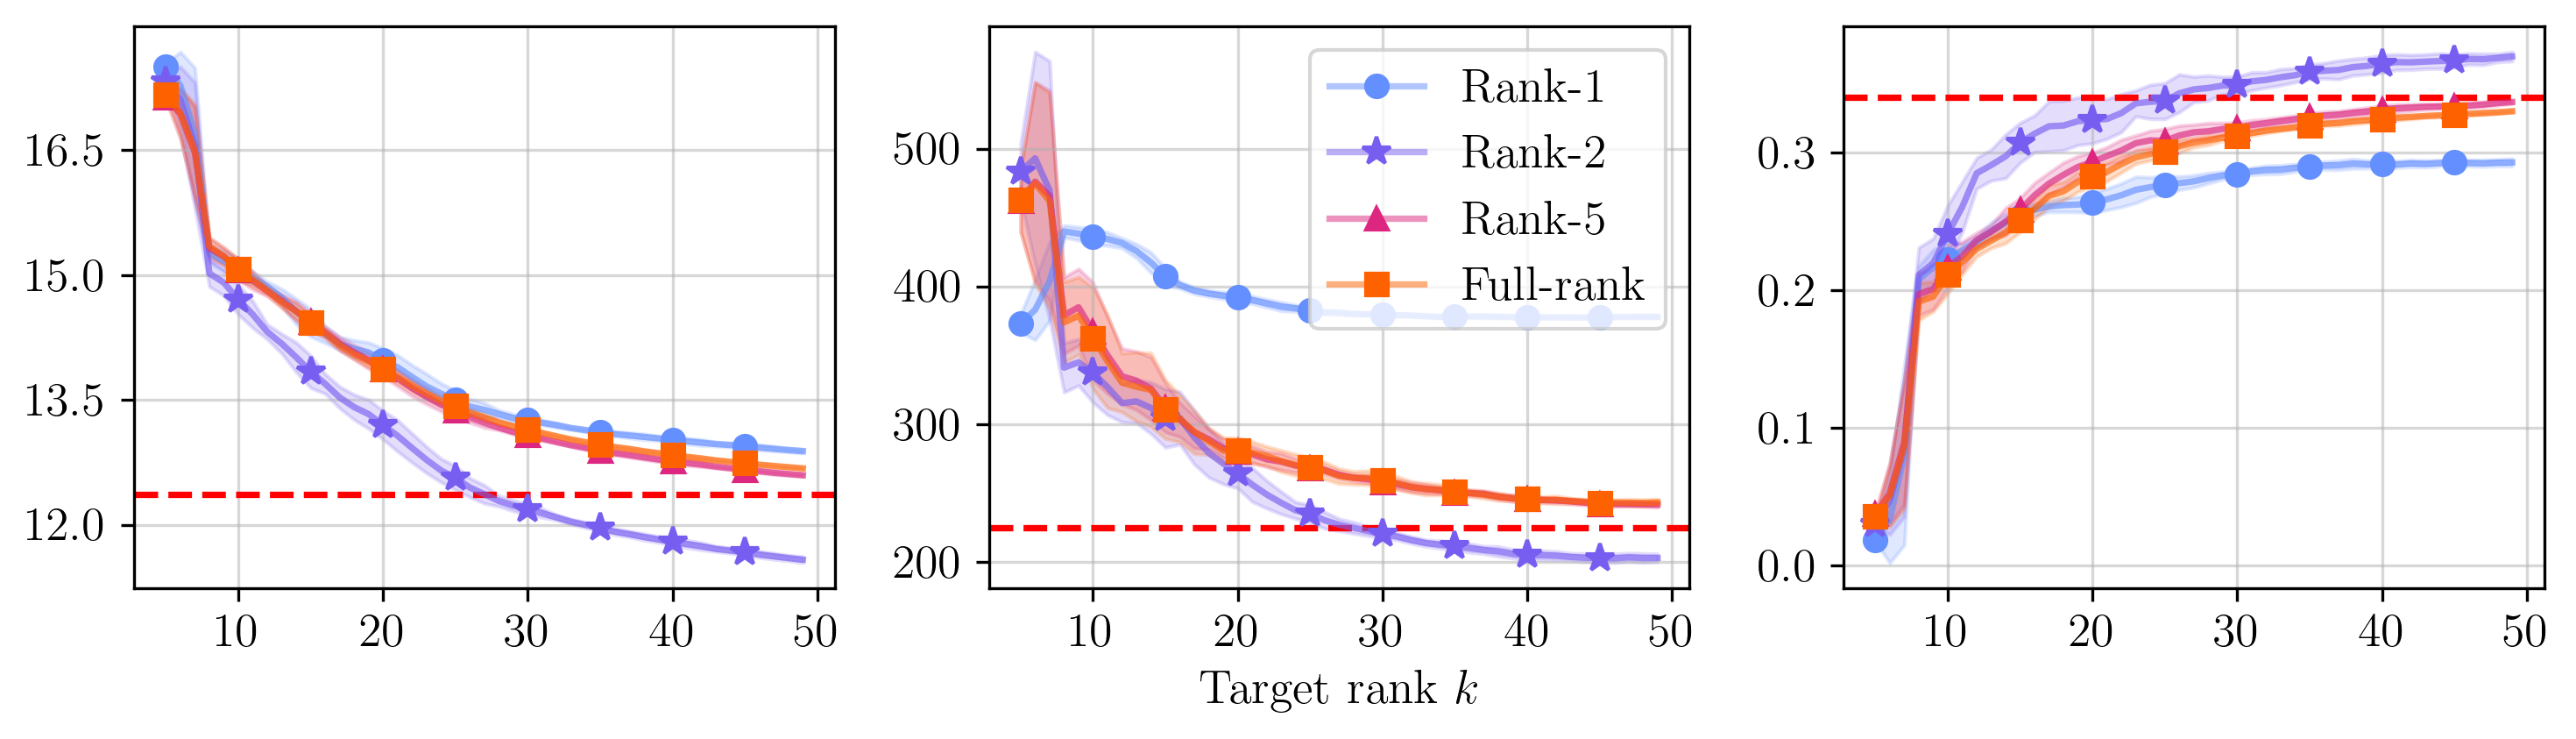
\includegraphics[width=\linewidth]{low_rank_solution_error_II.png}
    \caption{Problem II.}
    \label{fig:low_rank_solution_error_II}
\end{subfigure}

\caption{Reconstruction error vs.\ rSVD target rank $k$: full-rank Tikhonov solutions (rank-$k$ rSVD approximation of $K$ and $W$, Algorithm~\ref{alg:discrete_rsvd}) and DLRA-CG solutions at ranks $r = 1, 2, 5$ using the same approximation. Exact Tikhonov solution: dashed line. Columns: Euclidean norm (left), EMD (middle), AUC-IoU (right). Mean $\pm 1$ standard deviation over 30 runs.}
\label{fig:low_rank_solution_error}
\end{figure*}
Figure~\ref{fig:low_rank_different_r} shows DLRA-CG solutions for Problems~I and II at ranks $r = 1,\, 2,\, 5$. For Problem~I, the reconstruction error increases with rank, and at rank 5 the solution resembles the full-rank Tikhonov reconstruction (Figure~\ref{fig:test_problem_I}). For Problem~II, rank 2 is optimal, even though the true source is of rank 3 (reported in Section~\ref{sec:residuals_of_low_rank_solutions}; discussed in Section~\ref{sec:rank_as_a_regularization_parameter}). At rank 5 the reconstruction resembles the full-rank case~(Figure~\ref{fig:test_problem_II}).

Figure~\ref{fig:low_rank_solution_error} shows that for Problem~I, the rank-1 DLRA-CG solution achieves lower Euclidean and AUC-IoU error than the full rank rSVD solution. For EMD, the full-rank solution is better, possibly because the focused distribution of the rank-1 solution differs more from the flat true source than the smoother full-rank reconstruction. For Problem~II, the rank-2 solution outperforms rank-1, rank-5, and full-rank solutions across all metrics for $k > 10$. Reconstructions of rank 5 achieve approximately the same error as full-rank rSVD reconstructions.

As shown in Section~\ref{sec:target_rank_reconstruction}, full-rank rSVD solutions approach, but do not outperform the exact Tikhonov solution in the range $k \in [5,\,100]$ (Figure~\ref{fig:rsvd_over_k_II}). The low-rank solutions do: for Problem~I, the rank-1 solution surpasses the exact Tikhonov solution in Euclidean error from $k = 26$ and in AUC-IoU from $k = 31$, though not in EMD. For Problem~II, the rank-2 solution surpasses it across all metrics by $k = 28$.


\subsubsection{Residuals of low-rank solutions}\label{sec:residuals_of_low_rank_solutions}
\begin{figure*}[htbp]
    \centerline{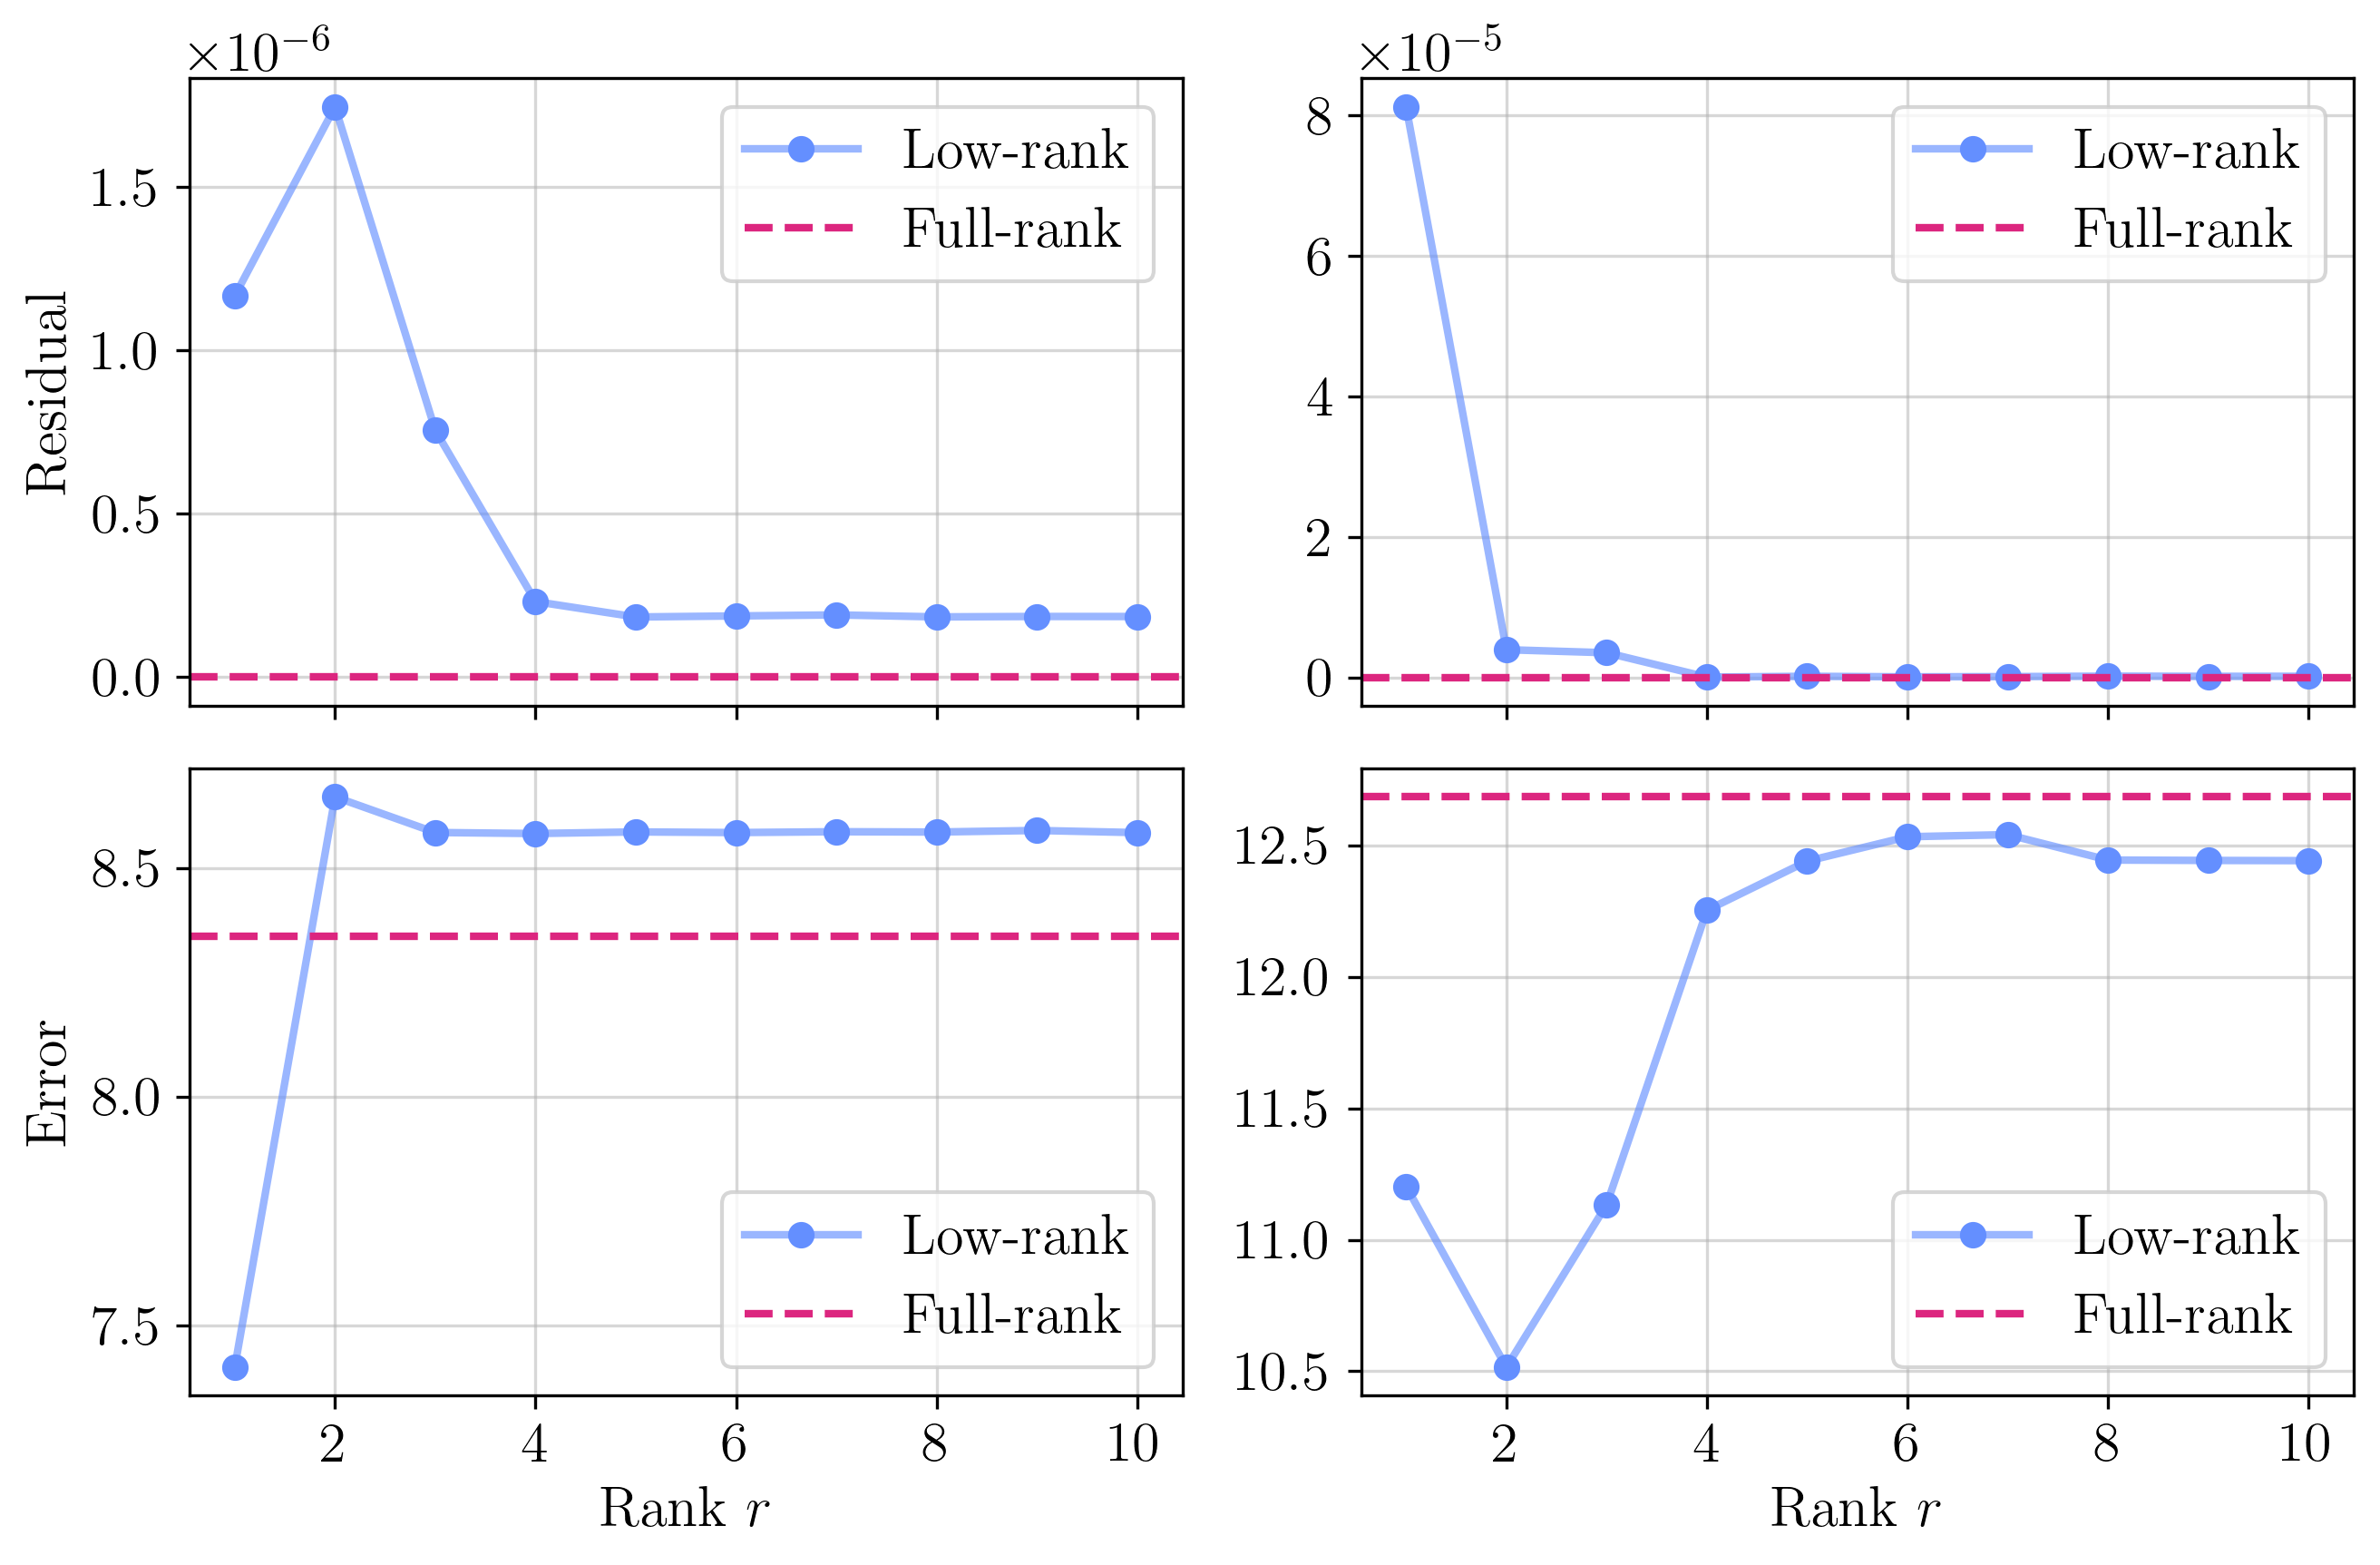
\includegraphics[width=1.0\textwidth]{low_rank_residual.png}}
\caption{The residuals (top row) and Euclidean error (bottom row) of low-rank solutions for ranks $r = 1,2,\dots,10$ using Problem~I (left) and II (right). Dashed line: residual/error of the full-rank solution. Solutions computed using Algorithm~\ref{alg:DLRA-CG} with $N_r = 10$.}
\label{fig:low_rank_residual}
\end{figure*}

For Problem~I, a rank-1 solution gives the best error, and for Problem~II, a rank-2 solution (Figure~\ref{fig:low_rank_residual}). The Problem~I residual rises and then falls with increasing rank, with no obvious connection to the optimal rank, while the Problem~II residual shows a sharp corner at the transition from rank~1 to rank~2. Using the residual curves could serve as a method for deciding a good rank, in particular to avoid choosing $r$ too small.


\subsubsection{Rate of convergence using preconditioners}\label{sec:rate_of_convergence_using_preconditioners}
\begin{figure*}[htbp]
    \centerline{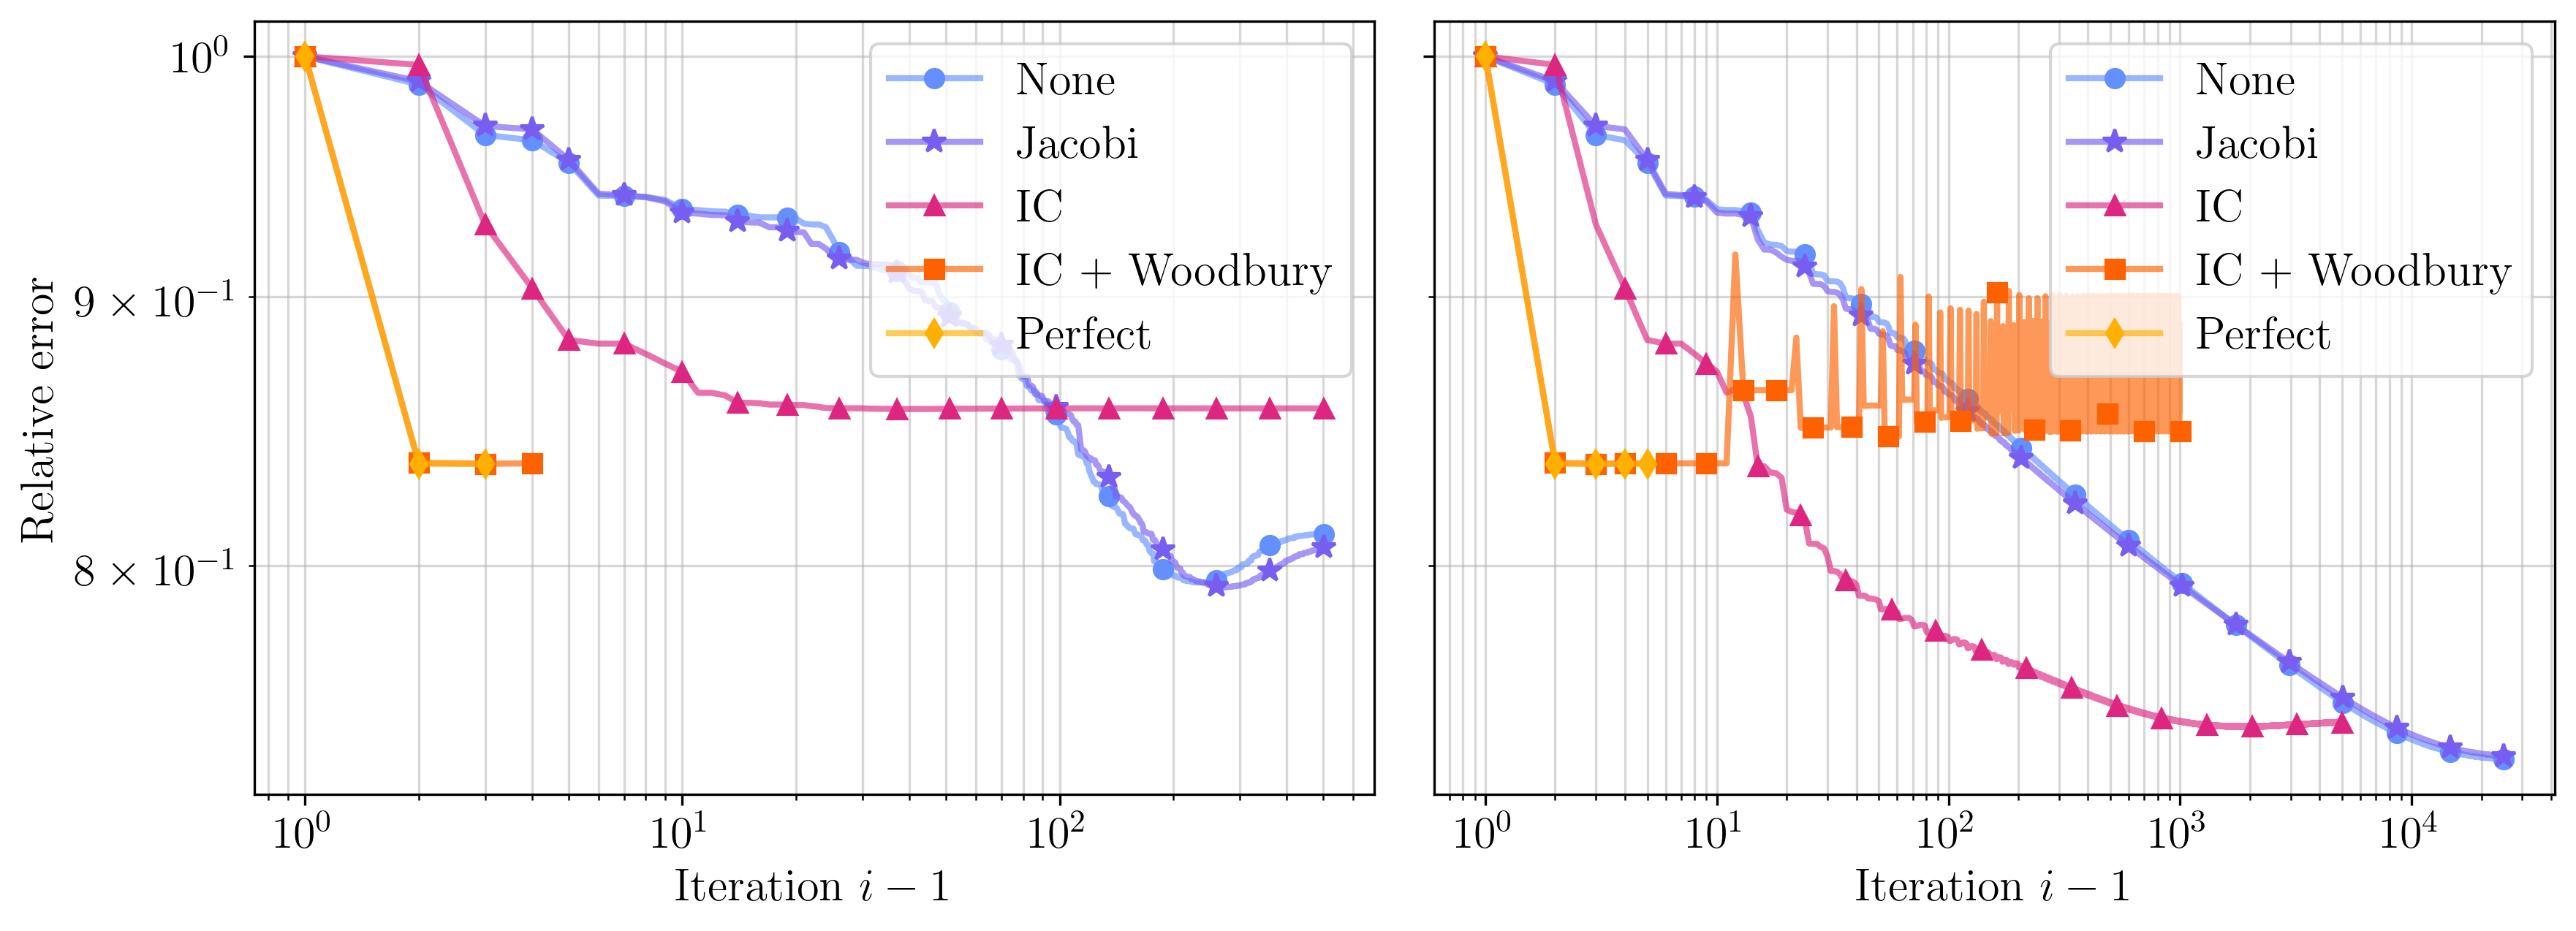
\includegraphics[width=1.0\textwidth]{number_of_iterations_preconditioners.png}}
    \caption{The relative reconstruction error $e^{(i)}$ versus iteration count using DLRA-PCG (Algorithm~\ref{alg:DLRA-PCG}) with four different preconditioners (Jacobi, IC, IC + Woodbury, Perfect) and no preconditioning (DLRA-CG). Left: no restarting. Right: restarting with $N_r = 10$. Problem~I was used.}
    \label{fig:number_of_iterations_preconditioners}
\end{figure*}
\begin{table}[!ht]
\centering
\begin{tabular}{llrrrr}
\hline
Preconditioner & $N_r$ & $< 0.90$ & $< 0.85$ & $< 0.80$ & $< 0.75$ \\
\hline
\multirow{3}{*}{None}  
& $\infty$ & 48 & 100 & 184 & \texttt{-} \\
& 25 & 54 & 249 & 958 & \texttt{-} \\
& 10 & 35 & 165 & 816 & 5941 \\
\hline
\multirow{3}{*}{Jacobi}
& $\infty$ & 43 & 112 & 204 & \texttt{-} \\
& 25 & 50 & 250 & 1042 & \texttt{-} \\
& 10 & 34 & 145 & 776 & 6518 \\
\hline
\multirow{3}{*}{IC}
& $\infty$ & 4 & \texttt{-} & \texttt{-} & \texttt{-} \\
& 25 & 4 & 28 & 57 & \texttt{-} \\
& 10 & 4 & 14 & 30 & 680 \\
\hline
IC+Woodbury & $\infty$ & 1 & 1 & \texttt{-} & \texttt{-} \\
Perfect     & $\infty$ & 1 & 1 & \texttt{-} & \texttt{-} \\
\hline
\end{tabular}
\caption{Number of iterations to reach a given relative reconstruction error $e^{(i)}$ using DLRA-PCG with different preconditioners and restart periods $N_r$ (Problem~I), where \texttt{-} indicates the threshold was not reached.}
\label{tab:convergence_iterations_precond}
\end{table}

The left panel of Figure~\ref{fig:number_of_iterations_preconditioners} shows that, except for Jacobi, using preconditioners speeds up the convergence significantly at the cost of higher error. IC, IC + Woodbury, and a perfect preconditioner show faster convergence compared to no preconditioning, but the final error is higher: $0.86$, $0.84$ and $0.84$ relative error, compared to $0.81$ for Jacobi and no preconditioning.

The right panel shows DLRA-PCG combined with restarting. For Jacobi, this gives a similar effect as restarted DLRA-CG: slower convergence but better final error. For the IC preconditioner, restarting reduces the final error steadily. The IC + Woodbury preconditioner shows worse results when combined with restarting: the error rises and the iterates diverge. Restarting has no effect on the perfect preconditioner.

The Jacobi, IC, and IC+Woodbury preconditioners have setup times of approximately $2$, $4$, and $11$ ms and per-iteration costs of $0.75$, $0.80$, and $1.17$ ms, compared to $0.74$ ms without preconditioning. IC with $N_r = 10$ reaches $e^{(i)} < 0.80$ and $< 0.75$ fastest among all tested combinations (Table~\ref{tab:convergence_iterations_precond}): 9 times fewer iterations and 8 times faster in computational time than without preconditioning. IC+Woodbury and Perfect reach $e^{(i)} < 0.85$ in a single iteration but stall there.


\subsubsection{Local minima}\label{sec:local_minima}
\begin{figure*}[htbp]
    \centerline{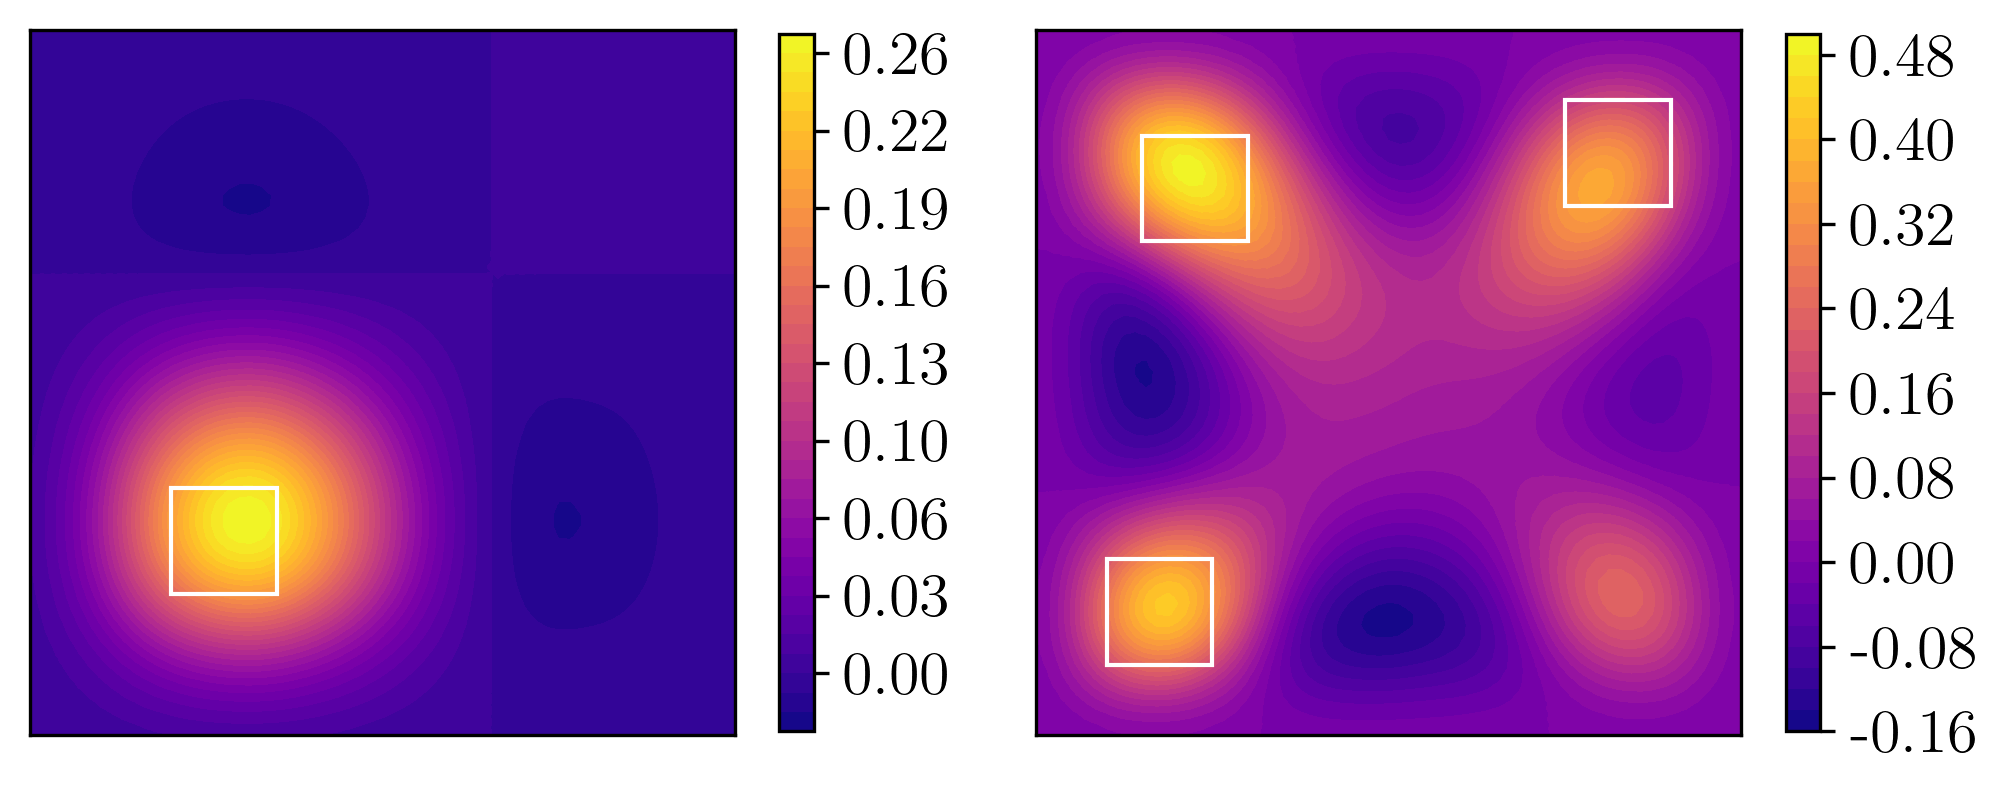
\includegraphics[width=0.80\textwidth]{diverged_solutions.png}}
    \caption{Suboptimal solutions using DLRA-PCG with IC + Woodbury preconditioner and $N_r = 10$. True sources outlined in white. Left: Problem~I, $r = 1$, $e^{(i)} = 0.85$. Right: Problem~II, $r = 2$, $e^{(i)} = 0.76$.}
    \label{fig:low_rank_diverged_solutions}
\end{figure*}
From Figure~\ref{fig:number_of_iterations_preconditioners} we saw that using DLRA-PCG with IC + Woodbury preconditioning and $N_r = 10$, the iterates diverged. Figure~\ref{fig:low_rank_diverged_solutions} shows these solutions after $500$ iterations. For Problem~I, the reconstruction is slightly shifted, with $e^{(i)} = 0.85$. For Problem~II, an incorrect source is seen in the lower right, and the relative error is $e^{(i)} = 0.76$.

For Problem~II, when using the suboptimal solution from the left panel of Figure~\ref{fig:low_rank_diverged_solutions} as the initial iterate $X^{(0)}$ for DLRA-CG and DLRA-PCG, the solvers were not able to escape this suboptimal solution (except when using a perfect preconditioner). This suggests that this point is a local minimum on the manifold of rank-$2$ matrices. Restarting resolved the problem. This issue was not observed for Problem~I. 

        % thesis ch. 5
\section{Discussion}
\label{sec:conclusions}

% Source: thesis/sections/6_discussion.tex and 7_conclusion.tex
%\section{Discussion}\label{sec:discussion}

%%%%%%%%%%%%%%%%%%%%%%%%%%%%%%%%%%%%%%%%%%%%%%%%%%%%%%%%%%%%%
% Matrix-free Randomized SVD Part 
%%%%%%%%%%%%%%%%%%%%%%%%%%%%%%%%%%%%%%%%%%%%%%%%%%%%%%%%%%%%%
\subsection{Matrix-free rSVD}
\subsubsection{Asymptotic analysis}
To explain the computational times and asymptotic behavior in Sections~\ref{sec:computational_time} and \ref{sec:computational_breakdown}, we examine the cost of forming $K$ and of Algorithm~\ref{alg:discrete_rsvd} in more detail. Standard dense SVD and QR costs throughout this and the following section follow \cite{golubMatrixComputations4th2013}.

For a 2D elliptic problem, the Cholesky factorization of $A_h$ and $M_\partial$ can be done in $\mathcal{O}(N^{3/2})$ and $\mathcal{O}(N_b^{3/2})$ computations, respectively (Section~\ref{sec:initial_matrix_factorizations}). The resulting triangular systems can be solved at the respective costs $\mathcal{O}(N \log N)$ and $\mathcal{O}(N_b \log N_b)$. Since $N_b \ll N$, we may disregard the factorization and triangular solves using $M_\partial$. 

The cost of computing $K = T A_h^{-1} M$ involves solving $N_b$ linear systems $A_h v_i = T^T e_i$ (Section~\ref{sec:rsvd}), each system costing $\mathcal{O}(N \log N)$ using a sparse Cholesky factorization of $A_h$. With $N_b \sim \sqrt{N}$, the cost therefore scales as $\mathcal{O}(N^{3/2} \log N)$, explaining the scaling of $t_K$ observed in the left panel of Figure~\ref{fig:rsvd_computational_time_comp}. The SVD of dense matrix $K \in \mathbb{R}^{N_b \times N}$ costs $\mathcal{O}(N_b^2 N) = \mathcal{O}(N^2)$, which is larger than $\mathcal{O}(N^{3/2} \log N)$, explaining $t_{\text{SVD}}$ in Figure~\ref{fig:rsvd_computational_time_comp}.

For the matrix-free rSVD (Algorithm~\ref{alg:discrete_rsvd}), factorizing $A_h$ costs $\mathcal{O}(N^{3/2})$, and is done once. Each application of $K$ and $K^*$ costs $\mathcal{O}(N \log N)$, totaling $\mathcal{O}(l N \log N)$. The SVD of the $l \times N$ matrix $B$ costs $\mathcal{O}(l^2 N)$, and the cost of the QR factorization of the small $N_b \times l$ matrix $Y$ is $\mathcal{O}(l^2 N_b)$, and may be disregarded. Hence, assuming two dimensions and an efficient sparse Cholesky factorization of $A_h$, Algorithm~\ref{alg:discrete_rsvd} costs
\begin{equation}\label{eq:rsvd_cost}
    \underbrace{\mathcal{O}(N^{3/2})}_{\text{setup}}
    + \underbrace{\mathcal{O}(l N \log N)}_{\substack{\text{forward and} \\ \text{adjoint solves}}}
    + \underbrace{\mathcal{O}(l^2 N)}_{\text{SVD of } B}.
\end{equation}

This is consistent with the results in the right panel of Figure~\ref{fig:rsvd_computational_time_comp}: $t_{\text{rSVD}}$ scales near-linearly on the observed range, matching the near-linear scaling of $\mathcal{O}(N \log N)$. Within the observed range, the $\mathcal{O}(lN\log N)$ solve cost dominates the one-time $\mathcal{O}(N^{3/2})$ setup (Figure~\ref{fig:rsvd_computational_breakdown}), and $N\log N$ is close enough to linear that $t_{\text{rSVD}}$ in Figure~\ref{fig:rsvd_computational_time_comp} appears near-linear.

Equation~\eqref{eq:rsvd_cost} also explains the cost breakdown in Figure~\ref{fig:rsvd_computational_breakdown}. For larger $k$, a larger share is taken up by the SVD stage, as predicted by $\mathcal{O}(l^2 N)$. For $k = 200$ ($l = k + p$), the largest considered target rank, we observed that as $N$ increases, the forward and adjoint solves start taking up a larger share of the time compared to the SVD of $B$, also consistent with Equation~\eqref{eq:rsvd_cost}. The cost $\mathcal{O}(l^2 N_b)$ of the QR-factorization $QR = Y$ is negligible, matching the results for all $k$ and $N$.


\subsubsection{Analysis of reconstruction error}\label{sec:analysis_of_reconstruction_error}
At target rank $k = 50$, rSVD reconstruction errors were within 0.5\% to 4\% of the exact Tikhonov solution in Euclidean norm and AUC-IoU (4\% to 39\% in EMD), with visually indistinguishable reconstructions (Section~\ref{sec:target_rank_reconstruction}, Figure~\ref{fig:test_problems_selected}).

To understand these results, we inspect the structure of $Y = K \Psi$. Following the setup of Halko et al. \cite[Sec.~9]{halkoFindingStructureRandomness2011}, let $K = U \Sigma V^T$ be the SVD of $K$, and partition $\Sigma$ as $\Sigma = \operatorname{diag}(\Sigma_1,\, \Sigma_2)$, where $\Sigma_1$ contains the $k$ first singular values of $K$, and $\Sigma_2$ the remainder. Correspondingly, partition the right singular vectors as $V = [V_1\,\, V_2]$, and write $K$ as
\begin{equation}\label{eq:rsvd_partitioned_1}
    K = U \begin{bmatrix}
    \Sigma_1 & \\ & \Sigma_2
    \end{bmatrix}
    \begin{bmatrix}
    V_1^T \\ V_2^T
    \end{bmatrix}.
\end{equation}
Right-multiplying by $\Psi$ and setting $\Psi_1 = V_1^T \Psi$ and $\Psi_2 = V_2^T \Psi$ gives
\begin{equation*}\label{eq:rsvd_partitioned_2}
    Y = U \begin{bmatrix}
    \Sigma_1 \Psi_1 \\
    \Sigma_2 \Psi_2
    \end{bmatrix}.
\end{equation*}
Here, $\Sigma_1 \Psi_1$ is the contribution from the $k$ dominant singular components we wish to recover, while $\Sigma_2 \Psi_2$ comes from the truncated tail and acts as a perturbation. By Theorem~10.5 in \cite{halkoFindingStructureRandomness2011}, if $\Psi \in \mathbb{R}^{N \times l}$ is a random Gaussian matrix, then
\begin{equation}\label{eq:rsvd_error_bound}
    \mathbb{E}\| K - K_k \|_F \le
    \gamma_k \sqrt{\sum_{i = k+1}^{N_b} \sigma_i^2},
\end{equation}
where $\mathbb{E}$ denotes the expected value, $\gamma_k = \sqrt{1 + k / (p - 1)}$, and $K_k$ is the rank-$k$ approximation obtained from the rSVD (Algorithm~\ref{alg:discrete_rsvd}).

When the singular values of $K$ decay rapidly, the perturbation $\Sigma_2 \Psi_2$ remains low and the sum in Equation~\eqref{eq:rsvd_error_bound} is small, resulting in a good rank-$k$ approximation. If the singular values decay more slowly, $\sum_{i=k+1}^{N_b} \sigma_i^2$ will be larger, and the expected error increases.

Since $K$ has rapidly decaying singular values
(Figure~\ref{fig:singular_values}), a target rank
$k \ll \operatorname{rank}(K) = N_b$ yields an accurate rank-$k$
approximation: the main actions of $K$ are captured in $\Sigma_1 \Psi_1$. This argument transfers to the weighted Tikhonov problem in Equation~\eqref{eq:discrete_inverse_problem}. Both $K$ and $W$ are approximated accurately at $k = 50$, keeping the reconstruction error within 4\% (Euclidean, AUC-IoU). Since the random sampling introduces some noise, the EMD shows a higher error, as it is more sensitive to low-amplitude noise.


\subsubsection{Effect of the test vector distribution}
\begin{figure*}[htbp]
    \centerline{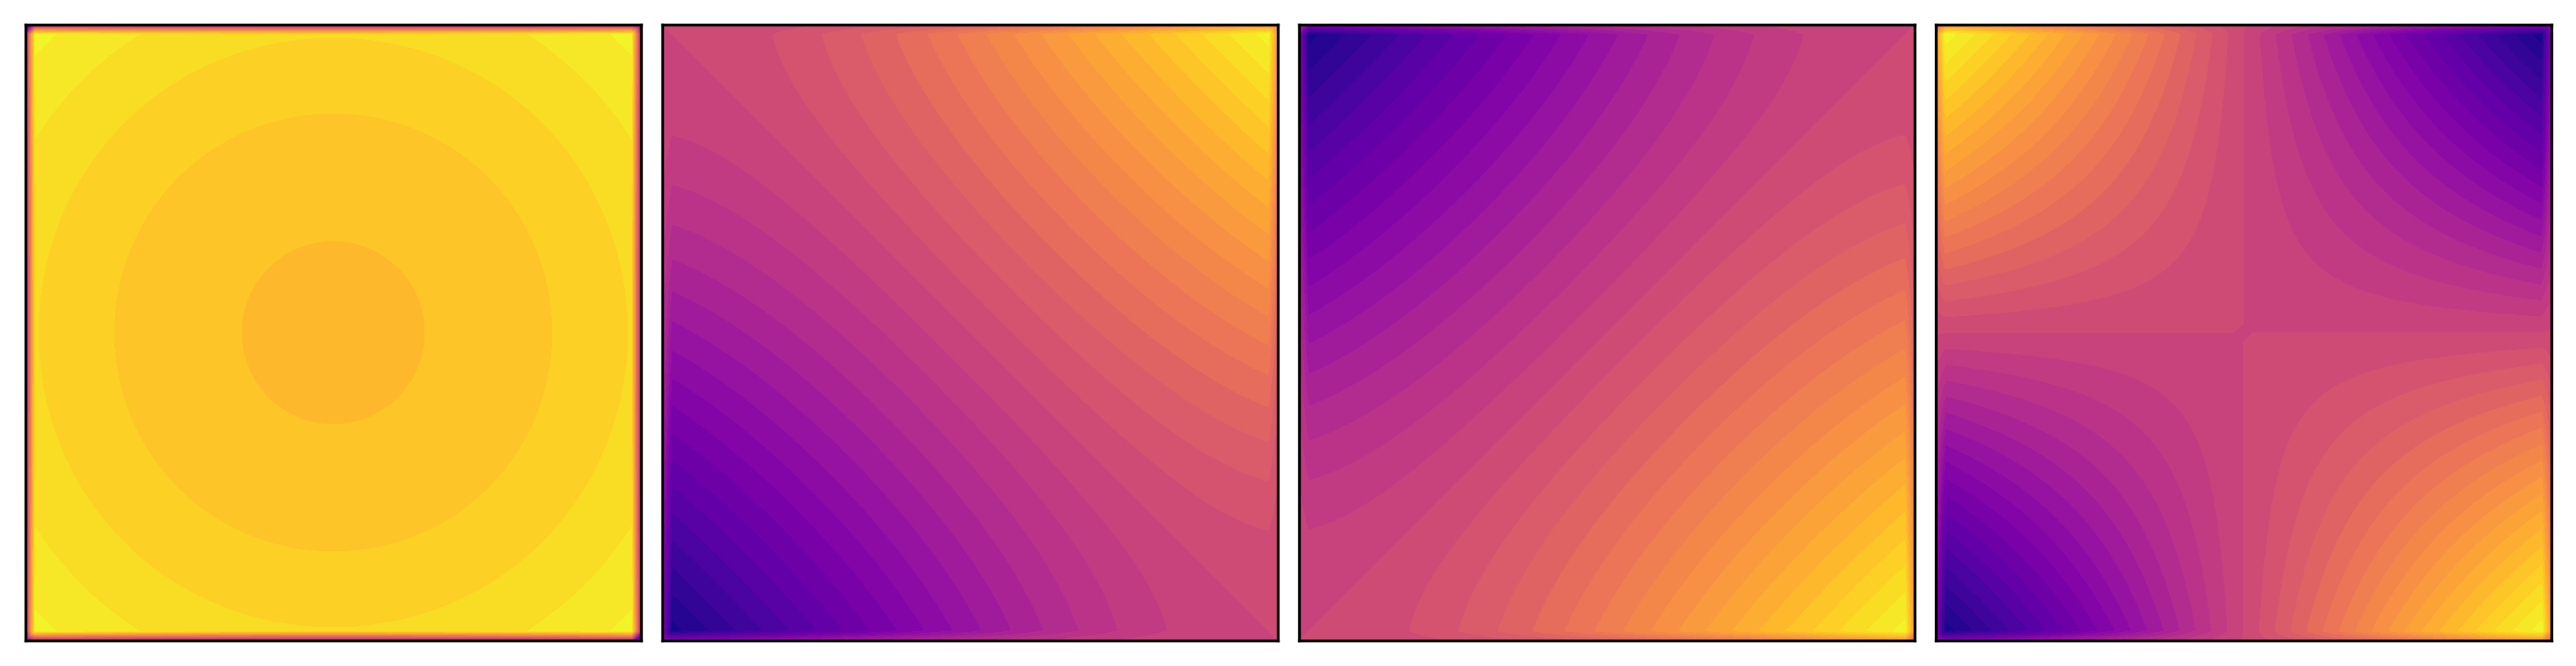
\includegraphics[width=1.0\textwidth]{singular_vectors_of_K.png}}
    \caption{The first four right singular vectors $v_1,\dots,v_4$ (shown in the same order) of the forward operator $K$ from Problem~I.}
    \label{fig:singular_vectors_of_K}
\end{figure*}
Some test vector distributions slightly reduce reconstruction error, with the Peak test vectors giving lower EMD than Gaussian or Rademacher (Section~\ref{sec:test_vector_distribution_effect_on_error}).

Consider a single sample $y = K \psi = U \Sigma V^T \psi$. In the best case, $\psi = a v_1$ with $a \neq 0$: then $V^T(a v_1) = a e_1$, $K(a v_1) = a \sigma_1 u_1$, and the QR factorization gives $Q = u_1$. More generally, choosing $k$ linearly independent $\psi_i \in \operatorname{span}\{ v_1,\dots,v_k \}$ gives $\operatorname{range}(Q) = \operatorname{span}\{u_1,\dots,u_k\}$ and the rank-$k$ projection $QQ^T K$ recovers the exact rank-$k$ SVD of $K$.

Figure~\ref{fig:singular_vectors_of_K} plots the first four right singular vectors of $K$. We see that they are smooth, more closely matching the Peak test vectors than the Gaussian or Rade\-macher test vectors, potentially explaining the small improvement in error.


\subsubsection{Independence from mesh resolution}
The reconstruction error is independent of the mesh resolution $N$ for fixed $k$ (Section~\ref{sec:mesh_resolution_effect_on_reconstruction_error}). The PDE solution at the boundary is smooth, so finer discretization produces more samples of the same smooth function without introducing new information about the source.

The continuous forward operator $\mathcal{K}$ has rapidly decaying singular values (Section~\ref{sec:ill_posedness}), and the discrete $K$ inherits this decay. As $N$ increases and $\operatorname{rank}(K) = N_b$ grows, the additional singular values are small with little new information.

The target rank $k$ can therefore be selected on a coarse mesh, where rSVD is inexpensive to run, and reused unchanged as the mesh is refined. This is a practical method for tuning $k$ when the final computation on a fine mesh is expensive.


\subsubsection{Estimation of singular values}
Let $\hat P = QQ^T$ with $Q$ produced by Algorithm~\ref{alg:discrete_rsvd}. This is an orthogonal projection onto $\operatorname{range}(Q)$, and $\hat P K$ is the projected matrix from which the rSVD approximation is obtained. The projector satisfies $\| \hat P z \| \le \| z \|$, meaning it shrinks vectors, so $\| \hat P K x  \| \le \|K x \|$ for every $x$. Consequently, $\hat P K$ stretches every vector at most as much as $K$ does, and singular values measure exactly this stretching. This is what we saw in Section~\ref{sec:approximation_of_singular_values}. By choosing a higher oversampling parameter $p$, $\operatorname{range}(Q)$ more closely matches $\operatorname{range}(K)$ (in particular, the $k$ first left singular vectors), and the underestimation reduces.

The captured subspace $\operatorname{range}(Q)$ depends on the random test vectors $\psi_i$, and so does the degree of underestimation. This is an active area of research. Lemma~4.2 and Theorem~4.3 of Gu \cite{guSubspaceIterationRandomization2015} provide lower bounds for the power-iteration method, which reduces to the plain rSVD used in Algorithm~\ref{alg:discrete_rsvd} when $q = 0$.


\subsubsection{Reconstructions under noisy data}
Choosing $k$ too large worsens reconstruction quality on noisy data (Section~\ref{sec:accuracy_on_noisy_data}), and the target rank acts as a regularization parameter in the same manner as the truncation rank of tSVD.

For a noisy measurement $\tilde y = y + \epsilon$, $y = K x$, we can write the minimum-norm least-squares solution as $x^* = K^+ \tilde y = K^+ y + K^+ \epsilon$ (Section~\ref{sec:svd}). Expanding in terms of the SVD components,
\begin{equation*}
    x^* = \sum_{i=1}^{N_b}
    \left(\frac{u_i^T y + u_i^T \epsilon}{\sigma_i}\right) v_i,
\end{equation*}
we see that the $i$-th component depends on the exact term $u_i^T y$ and the noise term $u_i^T \epsilon$. Components where $|u_i^T y| \le |u_i^T \epsilon|$ are dominated by noise, and the $\tfrac{1}{\sigma_i}$ factor amplifies this contribution. Assuming that the Picard condition \cite{hansen2010discrete} holds, $u_i^T y$ decays to zero as $i$ increases while $u_i^T \epsilon$ stays approximately constant, so for large $i$ every component is noise-dominated and amplified by a growing $\tfrac{1}{\sigma_i}$.

By truncating the $N_b - k$ terms of the solution, we remove the noisy SVD components. We wish to choose $k$ such that $|u_k^T y| > |u_k^T \epsilon|$ while $|u_{k+1}^T y| < |u_{k+1}^T \epsilon|$, removing only the noise-dominated SVD components $k+1,\, k+2,\dots,\, N_b$.

For the weighted Tikhonov solution, the reconstruction already has some regularization through $\lambda$, but the argument transfers. We found that the optimal $k$ values are approximately equal for both the rSVD and the tSVD. The rank is problem-dependent, and for our problems ranged from $k = 45$ to $k = 85$ by Euclidean norm. The EMD preferred a smaller $k$ ($20$ to $30$), since it is more sensitive to unwanted noise in the reconstruction, while the AUC-IoU generally preferred larger $k$ ($\ge 60$), since it focuses on segmentation overlap, which is less affected by noise.


%%%%%%%%%%%%%%%%%%%%%%%%%%%%%%%%%%%%%%%%%%%%%%%%%%%%%%%%%%%%%
% Dynamical Low-Rank Approximation using Conjugate Gradient 
%%%%%%%%%%%%%%%%%%%%%%%%%%%%%%%%%%%%%%%%%%%%%%%%%%%%%%%%%%%%%
\subsection{Dynamical low-rank approximation}
\subsubsection{Convergence of DLRA-CG}\label{sec:convergence_of_DLRA_CG}
Replacing the steepest descent search directions with directions $\{D^{(i)}\}$ from CG increased convergence significantly: DLRA-CG reached the relative error $e^{(i)} < 0.85$ approximately $210$ times faster than steepest descent (Section~\ref{sec:rate_of_convergence}).

In an unconstrained setting, the convergence of CG and steepest descent depends on the condition number $\kappa = \kappa(H)$, with larger $\kappa$ leading to slower convergence \cite{saadIterativeMethodsSparse2003}. If $x^*$ is the unconstrained minimizer of $\Phi(x)$ and $x^{(i)}$ the $i$-th iterate of CG, then by Theorem~6.29 in Saad \cite{saadIterativeMethodsSparse2003},
\begin{equation}\label{eq:convergence_of_CG}
    \| x^* - x^{(i)} \|_H \le 2 \left(
        \frac{\sqrt{\kappa} - 1}{\sqrt{\kappa} + 1}
    \right)^i
    \| x^* - x^{(0)} \|_H.
\end{equation}
If $\kappa$ is large, then $\tfrac{\sqrt{\kappa} - 1}{\sqrt{\kappa} + 1} \approx 1 - \tfrac{2}{\sqrt{\kappa}}$, compared to the slower convergence of steepest descent which converges as approximately $1 - \tfrac{2}{\kappa}$ \cite{saadIterativeMethodsSparse2003}.

The Hessian $H = F + S$ has a low-rank $F = K^T M_\partial K$ plus a sparse $S = \lambda^2 W^T M W$ structure (Section~\ref{sec:choice_of_preconditioner}). The rapid decay of singular values of $K$ makes $\kappa(H)$ depend on $\lambda$: the small eigenvalues of $H$ are mostly determined by $S$, whose eigenvalues are small when $\lambda$ is small. For example, at $\lambda = 0.1$, $\kappa(H) \approx 10^3$, and at  $\lambda = 10^{-4}$, $\kappa(H) \approx 10^9$.

The same argument partially transfers to DLRA-CG, as demonstrated by Table~\ref{tab:convergence_iterations}, since $\{D^{(i)}\}$ is generated by the same CG recurrence as in the unconstrained case. A formal convergence analysis of DLRA-CG that accounts for the projection and truncation remains an open problem.


\subsubsection{Semi-convergence and restarting}
\begin{figure}[htbp]
    \centering
    \begin{tikzpicture}[
        >=stealth,
        line width=0.9pt,
        every node/.style={font=\large}
    ]
    % Manifold M_r as a smooth curve
    \draw[thick] plot[smooth, domain=-2.8:2.8, samples=60]
        ({\x}, {0.22*\x*\x - 1});
    \node at (3, 0.9) {$\mathcal{M}_r$};

    % Tangent line at X^(i)
    \draw[dashed] (-2.8, -1) -- (3, -1);
    \node[right] at (3, -1) {$\mathcal{T}_{X^{(i)}}(\mathcal{M}_r)$};

    % Point X^(i)
    \coordinate (X) at (0, -1);
    \fill (X) circle (2.5pt);
    \node[below] at (X) {$X^{(i)}$};

    % \hat D^(i) = -grad Phi(X^(i)): true steepest descent direction at X^(i)
    \coordinate (Dhat) at (-1.4, 1);
    \draw[->, Green] (X) -- (Dhat);
    \node[above left, Green] at (Dhat) {$\hat D^{(i)}$};

    % Dotted projection from \hat D tip down onto the tangent line
    \draw[dotted, Green] (Dhat) -- (-1.4, -1);

    % P \hat D^(i): projection of \hat D onto T_{X^(i)} M_r (Riemannian descent direction)
    \coordinate (PDhat) at (-1.4, -1);
    \draw[->, Green] (X) -- (PDhat);
    \node[below, Green] at (PDhat) {$\mathcal{P}\hat D^{(i)}$};

    % D^(i): CG search direction, generated by the recurrence
    \coordinate (D) at (1.8, 1.4);
    \draw[->, Red] (X) -- (D);
    \node[above right, Red] at (D) {$D^{(i)}$};

    % Dotted projection from D tip down onto the tangent line
    \draw[dotted, Red] (D) -- (1.8, -1);

    % P D^(i): projection of D onto T_{X^(i)} M_r
    \coordinate (PD) at (1.8, -1);
    \draw[->, Red] (X) -- (PD);
    \node[below, Red] at (PD) {$\mathcal{P}D^{(i)}$};

    \end{tikzpicture}
    \caption{The CG search direction $D^{(i)}$ may disagree with the steepest-descent direction $\hat D^{(i)} = -\nabla\Phi(X^{(i)})$, so that their projections $\mathcal{P}D^{(i)}$ and $\mathcal{P}\hat D^{(i)}$ onto the tangent space $\mathcal{T}_{X^{(i)}}(\mathcal{M}_r)$ point in very different directions.}
    \label{fig:cg_direction_disagreement}
\end{figure}
DLRA-CG shows semi-convergence: initially the relative error reduces, and then it rises again before stalling (Section~\ref{sec:rate_of_convergence}). Restarted DLRA-CG avoids this, but shows slower convergence.

As discussed in Section~\ref{sec:restarted_cg}, the DLRA-CG algorithm constructs $(\alpha_i,\, G^{(i)},\, D^{(i)})$ independently of $X^{(i)}$. The search directions $\{D^{(i)}\}$ follow the trajectory of the full-rank solution $Y^{(i)}$, meaning $G^{(i)} = \nabla \Phi(Y^{(i)})$. When $i$ increases, $X^{(i)}$ and $Y^{(i)}$ may drift apart so that $G^{(i)}$ and the true gradient $\hat G^{(i)} = \nabla \Phi(X^{(i)})$ increasingly disagree. The projections of $D^{(i)}$ and $\hat D^{(i)} = -\hat G^{(i)}$,
\begin{equation*}
    \mathcal{P} D^{(i)}
    = \mathcal{P}_{X^{(i)}}(D^{(i)}),\quad
    \mathcal{P} \hat D^{(i)}
    = \mathcal{P}_{X^{(i)}}(\hat D^{(i)}),
\end{equation*}
may disagree to the point that the relative error $e^{(i)}$ rises again, resulting in semi-convergence. This is illustrated in Figure~\ref{fig:cg_direction_disagreement}.

Restarting sets $D^{(i)} = \hat D^{(i)}$, so the projected step $\mathcal{P}D^{(i)} = \mathcal{P}\hat D^{(i)}$ is the descent direction at $X^{(i)}$. As the iterations continue and $X^{(i)}$ drifts away from $Y^{(i)}$, this alignment gradually breaks down until the next restart. When the restart period $N_r$ is too small, the convergence of DLRA-CG will approach the steepest descent rate (at $N_r = 1$ they are equal), but choosing $N_r$ too large gives $X^{(i)}$ and $Y^{(i)}$ time to drift apart, so that semi-convergence re-appears.

An adaptive selection of $N_r$ could be considered, for example only restarting once the angle or relative difference between $G^{(i)}$ and the true gradient $\hat G^{(i)}$ is above some threshold.


\subsubsection{Rank as a regularization parameter}\label{sec:rank_as_a_regularization_parameter}
\begin{figure*}[htbp]
    \centerline{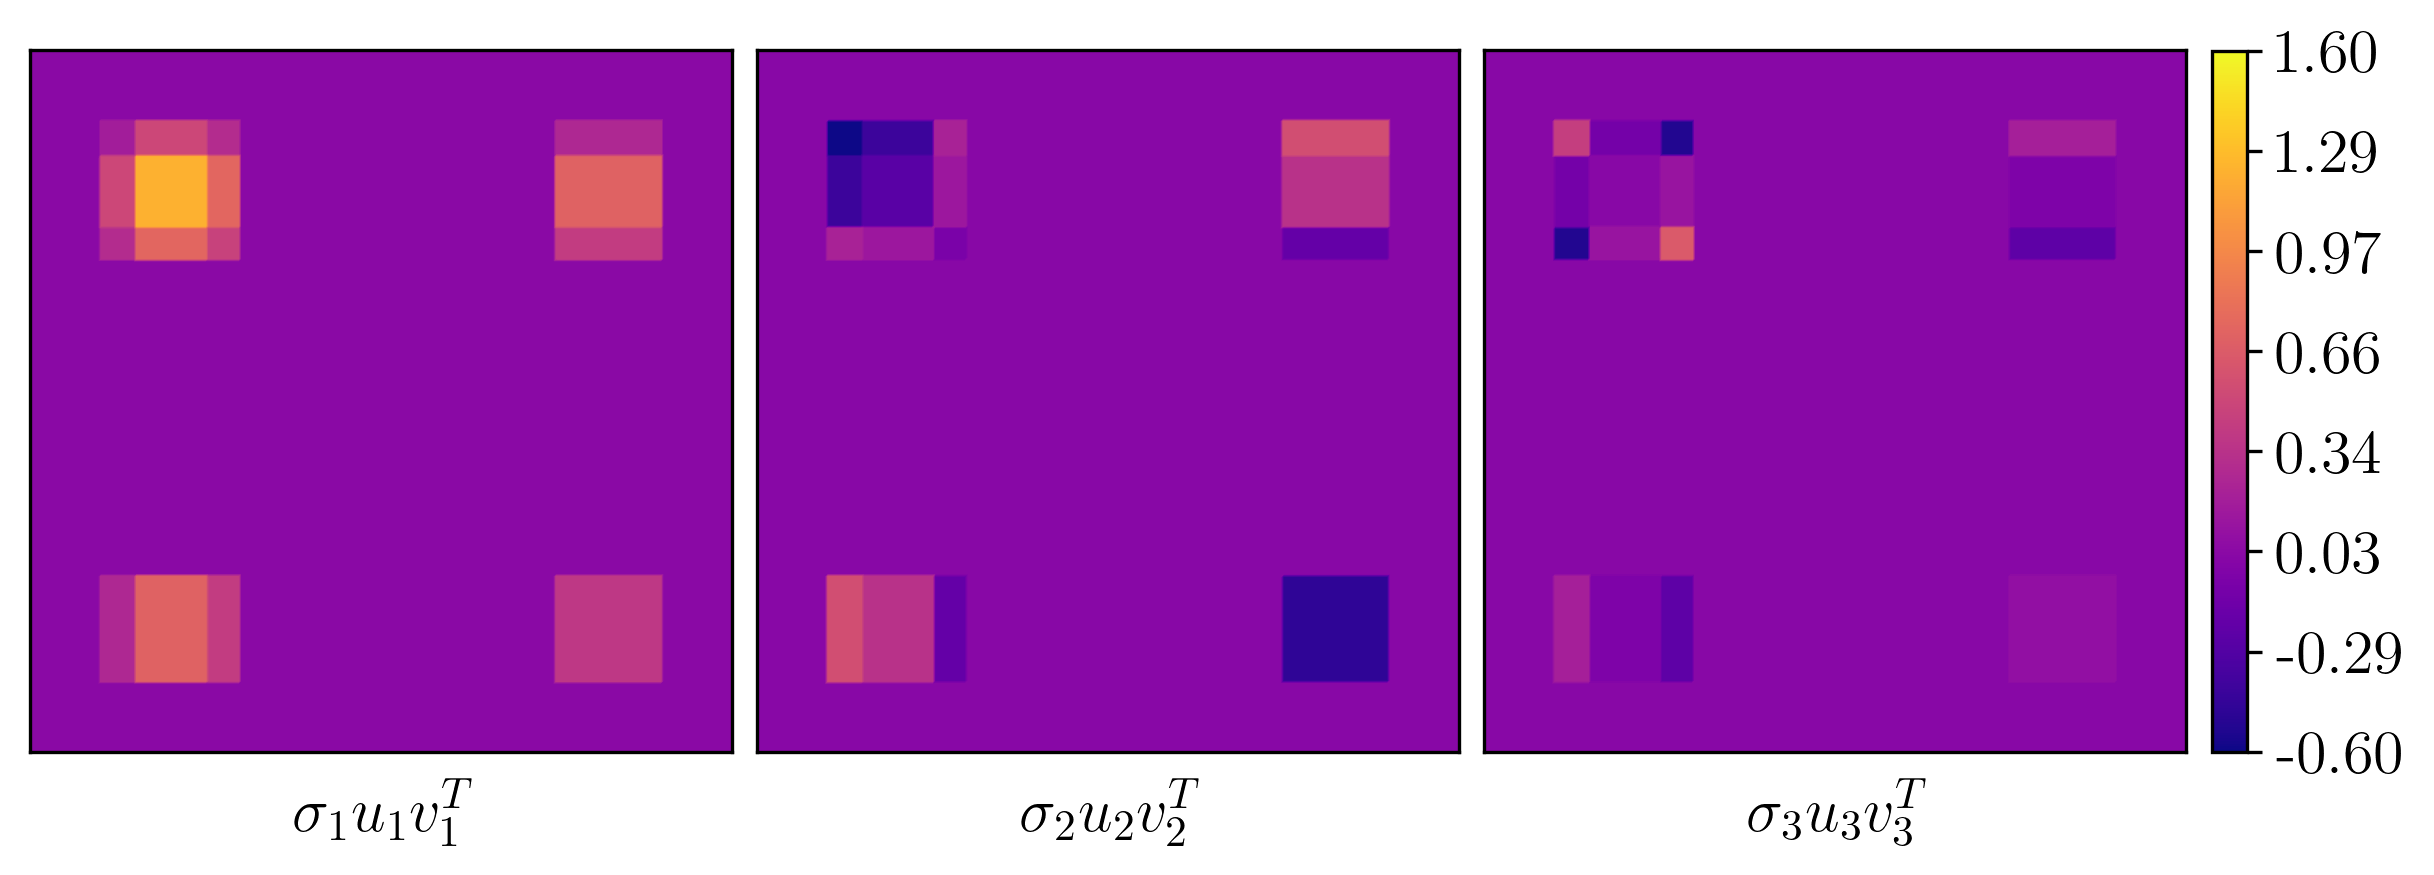
\includegraphics[width=1.0\textwidth]{outer_product_II.png}}
    \caption{The three individual rank-$1$ matrices whose sum makes up the source of Problem~II. Each rank-$1$ matrix is the outer product of a left and a right singular vector, scaled by their corresponding singular value.}
    \label{fig:outer_product_II}
\end{figure*}

The low-rank solutions outperformed exact weighted Tikhonov reconstructions (Section~\ref{sec:quality_of_the_low_rank_solutions}), but were sensitive to the choice of $r$: choosing $r$ slightly above optimal gave reconstructions resembling the full-rank case, while choosing $r$ too small introduced spurious sources for Problem~II
(Section~\ref{sec:effect_of_rank_on_reconstructions}).

The sources in Problems~I and II are of low rank and already live on $\mathcal{M}_r$. Each square source factors as an outer product of two vectors, giving a rank-$1$ matrix. The single source of Problem~I is therefore of rank~$1$, and the three sources of Problem~II sum to a matrix of rank~$3$, see Figure~\ref{fig:outer_product_II}. However, we found that a rank-$2$ approximation of this source yielded better reconstruction error. We interpret this as the rank constraint counteracting Tikhonov's oversmoothing: the discarded component is the most heavily smoothed but the least important of the three, so removing it is beneficial.

In practice, the residual as a function of rank served as a practical method for choosing $r$ in the case of multiple sources (Problem~II), but there was no obvious connection between the residual and the optimal rank for the simple rank-$1$ source of Problem~I (Section~\ref{sec:residuals_of_low_rank_solutions}).


\subsubsection{Effect of preconditioning}
We saw that preconditioning sped up convergence, but also raised the reconstruction error (Section~\ref{sec:rate_of_convergence_using_preconditioners}), and the iterates diverged when using an IC + Woodbury preconditioner together with restarting.

The convergence of CG depends on the condition number $\kappa(H)$. By using a preconditioner $P \approx H$, the condition number $\kappa(P^{-1} H)$ is reduced, and the convergence is sped up by Equation~\eqref{eq:convergence_of_CG}. As discussed in Section~\ref{sec:convergence_of_DLRA_CG}, $H$ has a large condition number, which makes preconditioning effective.

In the setting of DLRA-PCG, a stronger $P$ accelerates the convergence of the iterates $Y^{(i)}$ so that they reach the full-rank weighted Tikhonov solution in fewer iterations, leaving $X^{(i)}$ further behind on $\mathcal{M}_r$. This raises the error of the final $X^{(i)}$. In the case of the perfect preconditioner $P^{-1} = H^{-1}$, $Y^{(i)}$ reaches the full-rank solution in a single step, and $X^{(i)}$ is moved a single step in the projected direction and truncated to $\mathcal{M}_r$.

When using the IC preconditioner, the higher final error was resolved by restarting. With the IC + Woodbury preconditioner and restarting, however, the iterates $X^{(i)}$ diverge. Since $\mathcal{M}_r$ is non-convex \cite{absilOptimizationAlgorithmsMatrix2008}, $X^{(i)}$ may converge to a local minimum, as demonstrated in Section~\ref{sec:local_minima}, but we have no complete explanation.

\section{Conclusion}\label{sec:conclusion}
% Restatement
We studied a source identification problem with an elliptic PDE-constrained forward operator which suffers from rapid decay of singular values and a large nullspace, leading to ill-posedness. Standard Tikhonov regularization gives biased solutions concentrated near the domain boundary, and smooths solutions such that distinct sources blur together.

% Contribution
We introduced a matrix-free rSVD approach that computes a rank-$k$ approximation to the SVD of the forward operator, avoiding explicit formation, and making Elvetun and Nielsen's weighted Tikhonov approach applicable at large scale. We also introduced the DLRA-CG method to accelerate the convergence of DLRA and efficiently recover sparse sources.

% Key results
The matrix-free rSVD solved previously computationally infeasible problems without significant loss in reconstruction quality. For the problems studied, a target rank of approximately $50$ sufficed, independent of the mesh size $N$. On noisy data, the target rank acted as additional regularization, yielding comparable results to truncated SVD.
We also applied DLRA-CG to recover low-rank solutions, converging up to approximately $210$ times faster than DLRA with steepest descent in the tested problems. The solutions achieved lower reconstruction error and separated distinct sources more clearly than full-rank weighted Tikhonov. DLRA-CG showed semi-convergence, which was solved using restarting, at the cost of slower convergence. Preconditioning (DLRA-PCG) achieved significantly faster convergence but increased the reconstruction error. Restarting partially resolved the higher error but produced unstable results for the IC + Woodbury preconditioner.

% Limitations
The matrix-free rSVD was tested on a single elliptic PDE with simple two-dimensional geometries and square sources, and its performance on other operators or domains remains untested. For operators with a slow decay of singular values, the target rank $k$ must be larger, reducing the feasibility of the method. The random nature of the method gives varying reconstructions between runs, but this can be controlled by the oversampling parameter $p$.

The DLRA-CG method is sensitive to the choice of rank $r$, where too small a rank gives incorrect solutions while a rank only slightly above optimal gives a reconstruction resembling the full-rank case. Without restarting, it is unclear when to stop to avoid semi-convergence. However, using DLRA-CG with restarting requires choosing a restart period: too short and convergence approaches steepest descent, too long and semi-convergence returns. Preconditioning introduced further complications, where iterates converged toward non-optimal solutions, with the effect more severe for preconditioners that closely approximated the Hessian.

% Future work
Extending the matrix-free rSVD to other PDE types, three-dimensional domains, more complex sources, and other geometries would establish how broadly the results generalize. The method could be extended using power iteration, like Algorithm~4.3 in \cite{halkoFindingStructureRandomness2011}, for problems of slow spectral decay, or using an adaptive rank selection based on a specified tolerance, like Algorithm~4.2 in \cite{halkoFindingStructureRandomness2011}. It is however unclear how a tolerance for $K$ transfers to the reconstruction error.

For DLRA-CG, the rank-adaptive variant of Schotthöfer et al. \cite{schotthoferLowrankLotteryTickets2022} could be explored, which removes the need for manual rank selection by automatically adapting the rank of the iterates based on a threshold. Stopping criteria such as the discrepancy principle or the L-curve \cite{hansen2010discrete} could be used to address semi-convergence. Establishing a convergence theory for DLRA-CG remains an open problem, particularly regarding the effect of preconditioning.

% Final summary
Together, these contributions provide efficient low-rank methods for sparse source identification in large-scale PDE-constrained inverse problems.         % thesis ch. 6--7

\bibliographystyle{siamplain}
\bibliography{references}

\end{document}
